\documentclass{article} % For LaTeX2e
\usepackage{iclr2026_conference,times}

\usepackage{microtype}
\usepackage{hyperref}
\usepackage{url}
\usepackage{booktabs}

\usepackage{lineno}
\usepackage{graphicx}
\usepackage{tcolorbox}
\usepackage{tikz}
\usetikzlibrary{positioning, fit, arrows.meta, shapes.geometric}
\usepackage{wrapfig}
\usepackage{colortbl} % For row coloring
\usepackage[T1]{fontenc}

\usepackage{xcolor}
\usepackage{mdframed}
\usepackage{fancyvrb}
\usepackage{etoolbox}
\usepackage{changepage}

\usepackage{tikz}
\usepackage{multirow}
\usepackage{graphicx}
\usepackage{nicematrix} % Better handling of colored cells with multirow
\usepackage{rotating}
\usepackage{xcolor}
\usetikzlibrary{decorations.pathreplacing}

% Algorithm formatting
\usepackage{algorithm}
\usepackage{algpseudocode}
\newcommand{\diyi}[1]{{\color{red} Diyi: #1}}
\definecolor{darkblue}{rgb}{0, 0, 0.5}
\hypersetup{
	colorlinks=true,
	citecolor=darkblue,
	linkcolor=darkblue,
	urlcolor=darkblue
}
%%%%% NEW MATH DEFINITIONS %%%%%

\usepackage{amsmath, amsfonts, bm}

% Mark sections of captions for referring to divisions of figures
\newcommand{\figleft}{{\em (Left)}}
\newcommand{\figcenter}{{\em (Center)}}
\newcommand{\figright}{{\em (Right)}}
\newcommand{\figtop}{{\em (Top)}}
\newcommand{\figbottom}{{\em (Bottom)}}
\newcommand{\captiona}{{\em (a)}}
\newcommand{\captionb}{{\em (b)}}
\newcommand{\captionc}{{\em (c)}}
\newcommand{\captiond}{{\em (d)}}

% Highlight a newly defined term
\newcommand{\newterm}[1]{{\bf #1}}

% Figure reference, lower-case.
\def\figref#1{figure~\ref{#1}}
% Figure reference, capital. For start of sentence
\def\Figref#1{Figure~\ref{#1}} \def\twofigref#1#2{figures \ref{#1} and \ref{#2}}
\def\quadfigref#1#2#3#4{figures \ref{#1}, \ref{#2}, \ref{#3} and \ref{#4}}
% Section reference, lower-case.
\def\secref#1{section~\ref{#1}}
% Section reference, capital.
\def\Secref#1{Section~\ref{#1}}
% Reference to two sections.
\def\twosecrefs#1#2{sections \ref{#1} and \ref{#2}}
% Reference to three sections.
\def\secrefs#1#2#3{sections \ref{#1}, \ref{#2} and \ref{#3}}
% Reference to an equation, lower-case.
\def\eqref#1{equation~\ref{#1}}
% Reference to an equation, upper case
\def\Eqref#1{Equation~\ref{#1}}
% A raw reference to an equation---avoid using if possible
\def\plaineqref#1{\ref{#1}}
% Reference to a chapter, lower-case.
\def\chapref#1{chapter~\ref{#1}}
% Reference to an equation, upper case.
\def\Chapref#1{Chapter~\ref{#1}}
% Reference to a range of chapters
\def\rangechapref#1#2{chapters\ref{#1}--\ref{#2}}
% Reference to an algorithm, lower-case.
\def\algref#1{algorithm~\ref{#1}}
% Reference to an algorithm, upper case.
\def\Algref#1{Algorithm~\ref{#1}} \def\twoalgref#1#2{algorithms \ref{#1} and \ref{#2}}
\def\Twoalgref#1#2{Algorithms \ref{#1} and \ref{#2}}
% Reference to a part, lower case
\def\partref#1{part~\ref{#1}}
% Reference to a part, upper case
\def\Partref#1{Part~\ref{#1}} \def\twopartref#1#2{parts \ref{#1} and \ref{#2}}

\def\ceil#1{\lceil #1 \rceil} \def\floor#1{\lfloor #1 \rfloor} \def\1{\bm{1}}
\newcommand{\train}{\mathcal{D}}
\newcommand{\valid}{\mathcal{D_{\mathrm{valid}}}}
\newcommand{\test}{\mathcal{D_{\mathrm{test}}}}

\def\eps{{\epsilon}}

% Random variables
\def\reta{{\textnormal{$\eta$}}} \def\ra{{\textnormal{a}}} \def\rb{{\textnormal{b}}}
\def\rc{{\textnormal{c}}} \def\rd{{\textnormal{d}}} \def\re{{\textnormal{e}}} \def\rf{{\textnormal{f}}}
\def\rg{{\textnormal{g}}} \def\rh{{\textnormal{h}}} \def\ri{{\textnormal{i}}} \def\rj{{\textnormal{j}}}
\def\rk{{\textnormal{k}}} \def\rl{{\textnormal{l}}}
% rm is already a command, just don't name any random variables m
\def\rn{{\textnormal{n}}} \def\ro{{\textnormal{o}}} \def\rp{{\textnormal{p}}} \def\rq{{\textnormal{q}}}
\def\rr{{\textnormal{r}}} \def\rs{{\textnormal{s}}} \def\rt{{\textnormal{t}}} \def\ru{{\textnormal{u}}}
\def\rv{{\textnormal{v}}} \def\rw{{\textnormal{w}}} \def\rx{{\textnormal{x}}} \def\ry{{\textnormal{y}}}
\def\rz{{\textnormal{z}}}

% Random vectors
\def\rvepsilon{{\mathbf{\epsilon}}} \def\rvtheta{{\mathbf{\theta}}} \def\rva{{\mathbf{a}}}
\def\rvb{{\mathbf{b}}} \def\rvc{{\mathbf{c}}} \def\rvd{{\mathbf{d}}} \def\rve{{\mathbf{e}}}
\def\rvf{{\mathbf{f}}} \def\rvg{{\mathbf{g}}} \def\rvh{{\mathbf{h}}} \def\rvu{{\mathbf{i}}}
\def\rvj{{\mathbf{j}}} \def\rvk{{\mathbf{k}}} \def\rvl{{\mathbf{l}}} \def\rvm{{\mathbf{m}}}
\def\rvn{{\mathbf{n}}} \def\rvo{{\mathbf{o}}} \def\rvp{{\mathbf{p}}} \def\rvq{{\mathbf{q}}}
\def\rvr{{\mathbf{r}}} \def\rvs{{\mathbf{s}}} \def\rvt{{\mathbf{t}}} \def\rvu{{\mathbf{u}}}
\def\rvv{{\mathbf{v}}} \def\rvw{{\mathbf{w}}} \def\rvx{{\mathbf{x}}} \def\rvy{{\mathbf{y}}}
\def\rvz{{\mathbf{z}}}

% Elements of random vectors
\def\erva{{\textnormal{a}}} \def\ervb{{\textnormal{b}}} \def\ervc{{\textnormal{c}}}
\def\ervd{{\textnormal{d}}} \def\erve{{\textnormal{e}}} \def\ervf{{\textnormal{f}}}
\def\ervg{{\textnormal{g}}} \def\ervh{{\textnormal{h}}} \def\ervi{{\textnormal{i}}}
\def\ervj{{\textnormal{j}}} \def\ervk{{\textnormal{k}}} \def\ervl{{\textnormal{l}}}
\def\ervm{{\textnormal{m}}} \def\ervn{{\textnormal{n}}} \def\ervo{{\textnormal{o}}}
\def\ervp{{\textnormal{p}}} \def\ervq{{\textnormal{q}}} \def\ervr{{\textnormal{r}}}
\def\ervs{{\textnormal{s}}} \def\ervt{{\textnormal{t}}} \def\ervu{{\textnormal{u}}}
\def\ervv{{\textnormal{v}}} \def\ervw{{\textnormal{w}}} \def\ervx{{\textnormal{x}}}
\def\ervy{{\textnormal{y}}} \def\ervz{{\textnormal{z}}}

% Random matrices
\def\rmA{{\mathbf{A}}} \def\rmB{{\mathbf{B}}} \def\rmC{{\mathbf{C}}} \def\rmD{{\mathbf{D}}}
\def\rmE{{\mathbf{E}}} \def\rmF{{\mathbf{F}}} \def\rmG{{\mathbf{G}}} \def\rmH{{\mathbf{H}}}
\def\rmI{{\mathbf{I}}} \def\rmJ{{\mathbf{J}}} \def\rmK{{\mathbf{K}}} \def\rmL{{\mathbf{L}}}
\def\rmM{{\mathbf{M}}} \def\rmN{{\mathbf{N}}} \def\rmO{{\mathbf{O}}} \def\rmP{{\mathbf{P}}}
\def\rmQ{{\mathbf{Q}}} \def\rmR{{\mathbf{R}}} \def\rmS{{\mathbf{S}}} \def\rmT{{\mathbf{T}}}
\def\rmU{{\mathbf{U}}} \def\rmV{{\mathbf{V}}} \def\rmW{{\mathbf{W}}} \def\rmX{{\mathbf{X}}}
\def\rmY{{\mathbf{Y}}} \def\rmZ{{\mathbf{Z}}}

% Elements of random matrices
\def\ermA{{\textnormal{A}}} \def\ermB{{\textnormal{B}}} \def\ermC{{\textnormal{C}}}
\def\ermD{{\textnormal{D}}} \def\ermE{{\textnormal{E}}} \def\ermF{{\textnormal{F}}}
\def\ermG{{\textnormal{G}}} \def\ermH{{\textnormal{H}}} \def\ermI{{\textnormal{I}}}
\def\ermJ{{\textnormal{J}}} \def\ermK{{\textnormal{K}}} \def\ermL{{\textnormal{L}}}
\def\ermM{{\textnormal{M}}} \def\ermN{{\textnormal{N}}} \def\ermO{{\textnormal{O}}}
\def\ermP{{\textnormal{P}}} \def\ermQ{{\textnormal{Q}}} \def\ermR{{\textnormal{R}}}
\def\ermS{{\textnormal{S}}} \def\ermT{{\textnormal{T}}} \def\ermU{{\textnormal{U}}}
\def\ermV{{\textnormal{V}}} \def\ermW{{\textnormal{W}}} \def\ermX{{\textnormal{X}}}
\def\ermY{{\textnormal{Y}}} \def\ermZ{{\textnormal{Z}}}

% Vectors
\def\vzero{{\bm{0}}} \def\vone{{\bm{1}}} \def\vmu{{\bm{\mu}}} \def\vtheta{{\bm{\theta}}}
\def\va{{\bm{a}}} \def\vb{{\bm{b}}} \def\vc{{\bm{c}}} \def\vd{{\bm{d}}} \def\ve{{\bm{e}}}
\def\vf{{\bm{f}}} \def\vg{{\bm{g}}} \def\vh{{\bm{h}}} \def\vi{{\bm{i}}} \def\vj{{\bm{j}}}
\def\vk{{\bm{k}}} \def\vl{{\bm{l}}} \def\vm{{\bm{m}}} \def\vn{{\bm{n}}} \def\vo{{\bm{o}}}
\def\vp{{\bm{p}}} \def\vq{{\bm{q}}} \def\vr{{\bm{r}}} \def\vs{{\bm{s}}} \def\vt{{\bm{t}}}
\def\vu{{\bm{u}}} \def\vv{{\bm{v}}} \def\vw{{\bm{w}}} \def\vx{{\bm{x}}} \def\vy{{\bm{y}}}
\def\vz{{\bm{z}}}

% Elements of vectors
\def\evalpha{{\alpha}} \def\evbeta{{\beta}} \def\evepsilon{{\epsilon}} \def\evlambda{{\lambda}}
\def\evomega{{\omega}} \def\evmu{{\mu}} \def\evpsi{{\psi}} \def\evsigma{{\sigma}}
\def\evtheta{{\theta}} \def\eva{{a}} \def\evb{{b}} \def\evc{{c}} \def\evd{{d}} \def\eve{{e}}
\def\evf{{f}} \def\evg{{g}} \def\evh{{h}} \def\evi{{i}} \def\evj{{j}} \def\evk{{k}}
\def\evl{{l}} \def\evm{{m}} \def\evn{{n}} \def\evo{{o}} \def\evp{{p}} \def\evq{{q}}
\def\evr{{r}} \def\evs{{s}} \def\evt{{t}} \def\evu{{u}} \def\evv{{v}} \def\evw{{w}}
\def\evx{{x}} \def\evy{{y}} \def\evz{{z}}

% Matrix
\def\mA{{\bm{A}}} \def\mB{{\bm{B}}} \def\mC{{\bm{C}}} \def\mD{{\bm{D}}} \def\mE{{\bm{E}}}
\def\mF{{\bm{F}}} \def\mG{{\bm{G}}} \def\mH{{\bm{H}}} \def\mI{{\bm{I}}} \def\mJ{{\bm{J}}}
\def\mK{{\bm{K}}} \def\mL{{\bm{L}}} \def\mM{{\bm{M}}} \def\mN{{\bm{N}}} \def\mO{{\bm{O}}}
\def\mP{{\bm{P}}} \def\mQ{{\bm{Q}}} \def\mR{{\bm{R}}} \def\mS{{\bm{S}}} \def\mT{{\bm{T}}}
\def\mU{{\bm{U}}} \def\mV{{\bm{V}}} \def\mW{{\bm{W}}} \def\mX{{\bm{X}}} \def\mY{{\bm{Y}}}
\def\mZ{{\bm{Z}}} \def\mBeta{{\bm{\beta}}} \def\mPhi{{\bm{\Phi}}} \def\mLambda{{\bm{\Lambda}}}
\def\mSigma{{\bm{\Sigma}}}

% Tensor
\DeclareMathAlphabet{\mathsfit}{\encodingdefault}{\sfdefault}{m}{sl}
\SetMathAlphabet{\mathsfit}{bold}{\encodingdefault}{\sfdefault}{bx}{n}
\newcommand{\tens}[1]{\bm{\mathsfit{#1}}}
\def\tA{{\tens{A}}} \def\tB{{\tens{B}}} \def\tC{{\tens{C}}} \def\tD{{\tens{D}}}
\def\tE{{\tens{E}}} \def\tF{{\tens{F}}} \def\tG{{\tens{G}}} \def\tH{{\tens{H}}}
\def\tI{{\tens{I}}} \def\tJ{{\tens{J}}} \def\tK{{\tens{K}}} \def\tL{{\tens{L}}}
\def\tM{{\tens{M}}} \def\tN{{\tens{N}}} \def\tO{{\tens{O}}} \def\tP{{\tens{P}}}
\def\tQ{{\tens{Q}}} \def\tR{{\tens{R}}} \def\tS{{\tens{S}}} \def\tT{{\tens{T}}}
\def\tU{{\tens{U}}} \def\tV{{\tens{V}}} \def\tW{{\tens{W}}} \def\tX{{\tens{X}}}
\def\tY{{\tens{Y}}} \def\tZ{{\tens{Z}}}

% Graph
\def\gA{{\mathcal{A}}} \def\gB{{\mathcal{B}}} \def\gC{{\mathcal{C}}} \def\gD{{\mathcal{D}}}
\def\gE{{\mathcal{E}}} \def\gF{{\mathcal{F}}} \def\gG{{\mathcal{G}}} \def\gH{{\mathcal{H}}}
\def\gI{{\mathcal{I}}} \def\gJ{{\mathcal{J}}} \def\gK{{\mathcal{K}}} \def\gL{{\mathcal{L}}}
\def\gM{{\mathcal{M}}} \def\gN{{\mathcal{N}}} \def\gO{{\mathcal{O}}} \def\gP{{\mathcal{P}}}
\def\gQ{{\mathcal{Q}}} \def\gR{{\mathcal{R}}} \def\gS{{\mathcal{S}}} \def\gT{{\mathcal{T}}}
\def\gU{{\mathcal{U}}} \def\gV{{\mathcal{V}}} \def\gW{{\mathcal{W}}} \def\gX{{\mathcal{X}}}
\def\gY{{\mathcal{Y}}} \def\gZ{{\mathcal{Z}}}

% Sets
\def\sA{{\mathbb{A}}} \def\sB{{\mathbb{B}}} \def\sC{{\mathbb{C}}} \def\sD{{\mathbb{D}}}
% Don't use a set called E, because this would be the same as our symbol
% for expectation.
\def\sF{{\mathbb{F}}} \def\sG{{\mathbb{G}}} \def\sH{{\mathbb{H}}} \def\sI{{\mathbb{I}}}
\def\sJ{{\mathbb{J}}} \def\sK{{\mathbb{K}}} \def\sL{{\mathbb{L}}} \def\sM{{\mathbb{M}}}
\def\sN{{\mathbb{N}}} \def\sO{{\mathbb{O}}} \def\sP{{\mathbb{P}}} \def\sQ{{\mathbb{Q}}}
\def\sR{{\mathbb{R}}} \def\sS{{\mathbb{S}}} \def\sT{{\mathbb{T}}} \def\sU{{\mathbb{U}}}
\def\sV{{\mathbb{V}}} \def\sW{{\mathbb{W}}} \def\sX{{\mathbb{X}}} \def\sY{{\mathbb{Y}}}
\def\sZ{{\mathbb{Z}}}

% Entries of a matrix
\def\emLambda{{\Lambda}} \def\emA{{A}} \def\emB{{B}} \def\emC{{C}} \def\emD{{D}}
\def\emE{{E}} \def\emF{{F}} \def\emG{{G}} \def\emH{{H}} \def\emI{{I}} \def\emJ{{J}}
\def\emK{{K}} \def\emL{{L}} \def\emM{{M}} \def\emN{{N}} \def\emO{{O}} \def\emP{{P}}
\def\emQ{{Q}} \def\emR{{R}} \def\emS{{S}} \def\emT{{T}} \def\emU{{U}} \def\emV{{V}}
\def\emW{{W}} \def\emX{{X}} \def\emY{{Y}} \def\emZ{{Z}} \def\emSigma{{\Sigma}}

% entries of a tensor
% Same font as tensor, without \bm wrapper
\newcommand{\etens}[1]{\mathsfit{#1}}
\def\etLambda{{\etens{\Lambda}}} \def\etA{{\etens{A}}} \def\etB{{\etens{B}}}
\def\etC{{\etens{C}}} \def\etD{{\etens{D}}} \def\etE{{\etens{E}}} \def\etF{{\etens{F}}}
\def\etG{{\etens{G}}} \def\etH{{\etens{H}}} \def\etI{{\etens{I}}} \def\etJ{{\etens{J}}}
\def\etK{{\etens{K}}} \def\etL{{\etens{L}}} \def\etM{{\etens{M}}} \def\etN{{\etens{N}}}
\def\etO{{\etens{O}}} \def\etP{{\etens{P}}} \def\etQ{{\etens{Q}}} \def\etR{{\etens{R}}}
\def\etS{{\etens{S}}} \def\etT{{\etens{T}}} \def\etU{{\etens{U}}} \def\etV{{\etens{V}}}
\def\etW{{\etens{W}}} \def\etX{{\etens{X}}} \def\etY{{\etens{Y}}} \def\etZ{{\etens{Z}}}

% The true underlying data generating distribution
\newcommand{\pdata}{p_{\rm{data}}}
% The empirical distribution defined by the training set
\newcommand{\ptrain}{\hat{p}_{\rm{data}}}
\newcommand{\Ptrain}{\hat{P}_{\rm{data}}}
% The model distribution
\newcommand{\pmodel}{p_{\rm{model}}}
\newcommand{\Pmodel}{P_{\rm{model}}}
\newcommand{\ptildemodel}{\tilde{p}_{\rm{model}}}
% Stochastic autoencoder distributions
\newcommand{\pencode}{p_{\rm{encoder}}}
\newcommand{\pdecode}{p_{\rm{decoder}}}
\newcommand{\precons}{p_{\rm{reconstruct}}}

\newcommand{\laplace}{\mathrm{Laplace}} % Laplace distribution

\newcommand{\E}{\mathbb{E}}
\newcommand{\Ls}{\mathcal{L}}
\newcommand{\R}{\mathbb{R}}
\newcommand{\emp}{\tilde{p}}
\newcommand{\lr}{\alpha}
\newcommand{\reg}{\lambda}
\newcommand{\rect}{\mathrm{rectifier}}
\newcommand{\softmax}{\mathrm{softmax}}
\newcommand{\sigmoid}{\sigma}
\newcommand{\softplus}{\zeta}
\newcommand{\KL}{D_{\mathrm{KL}}}
\newcommand{\Var}{\mathrm{Var}}
\newcommand{\standarderror}{\mathrm{SE}}
\newcommand{\Cov}{\mathrm{Cov}}
% Wolfram Mathworld says $L^2$ is for function spaces and $\ell^2$ is for vectors
% But then they seem to use $L^2$ for vectors throughout the site, and so does
% wikipedia.
\newcommand{\normlzero}{L^0}
\newcommand{\normlone}{L^1}
\newcommand{\normltwo}{L^2}
\newcommand{\normlp}{L^p}
\newcommand{\normmax}{L^\infty}

\newcommand{\parents}{Pa} % See usage in notation.tex. Chosen to match Daphne's book.

\DeclareMathOperator*{\argmax}{arg\,max}
\DeclareMathOperator*{\argmin}{arg\,min}

\DeclareMathOperator{\sign}{sign}
\DeclareMathOperator{\Tr}{Tr}
\let\ab\allowbreak

\usepackage{array}
\newcolumntype{C}[1]{>{\centering\arraybackslash}p{#1}}

\title{AutoLibra: Agent Metric Induction from Open-Ended Human Feedback}
% Authors must not appear in the submitted version. They should be hidden
% as long as the \colmfinalcopy macro remains commented out below.
% Non-anonymous submissions will be rejected without review.

\author{Hao Zhu\raisebox{0.5em}{
\includegraphics[height=1em]{figs/scale.png}} Phil
Cuvin\raisebox{0.5em}{
\includegraphics[height=1em]{figs/microscope.png}} Xinkai
Yu\raisebox{0.5em}{
\includegraphics[height=1em]{figs/ladder.png}} Charlotte Ka Yee
Yan\raisebox{0.5em}{
\includegraphics[height=1em]{figs/scale.png}} Jason Zhang\raisebox{0.5em}{
\includegraphics[
	height=1em
]{figs/scale.png}} Diyi Yang\raisebox{0.5em}{
\includegraphics[height=1em]{
	figs/scale.png
}}\\ \raisebox{0.5em}{
\includegraphics[height=1em]{figs/scale.png}}Stanford
University \raisebox{0.5em}{
\includegraphics[height=1em]{figs/microscope.png}}University
of Toronto \raisebox{0.5em}{
\includegraphics[height=1em]{figs/ladder.png}}University
of Pennsylvania\\ \texttt{\{zhuhao,ckyy,jasonbz,diyiy\}@stanford.edu}\\ \texttt{philippe.cuvin@mail.utoronto.ca},
\texttt{xinkaiyu@sas.upenn.edu}\\\\
\href{https://github.com/Open-Social-World/autolibra}{Code}\quad\href{https://huggingface.co/datasets/open-social-world/autolibra}{Data}\quad
Website: \url{https://autolibra.opensocial.world} }
% The \author macro works with any number of authors. There are two commands
% used to separate the names and addresses of multiple authors: \And and \AND.
%
% Using \And between authors leaves it to \LaTeX{} to determine where to break
% the lines. Using \AND forces a linebreak at that point. So, if \LaTeX{}
% puts 3 of 4 authors names on the first line, and the last on the second
% line, try using \AND instead of \And before the third author name.

\newcommand{\fix}{\marginpar{FIX}}
\newcommand{\new}{\marginpar{NEW}}

\def\month{06} % Insert correct month for camera-ready version
\def\year{2025} % Insert correct year for camera-ready version
\def\openreview{\url{https://openreview.net/forum?id=XXXX}} % Insert correct link to OpenReview for camera-ready version

\begin{document}
	\maketitle

	\begin{abstract}
		Agents are predominantly evaluated and optimized via task success metrics,
		which are coarse, rely on manual design from experts, and fail to reward
		intermediate emergent behaviors. We propose \emph{AutoLibra} \protect
		
\includegraphics[height=1em]{figs/scale.png}, a framework for agent evaluation,
        that transforms open-ended human feedback
		\emph{e.g.} ``\textsl{If you find that the button is disabled, don't click it
		again}'', or ``\textsl{This agent has too much autonomy to decide what to do
		on its own}'' into metrics for evaluating fine-grained behaviors in agent trajectories.
		AutoLibra accomplishes this by grounding feedback to an agent's behavior, clustering
		similar positive and negative behaviors, and creating concrete metrics with
		clear definitions and concrete examples, which can be used for prompting LLM-as-a-Judge
		as evaluators. We further propose two \emph{meta-metrics} to evaluate the alignment
		of a set of (induced) metrics with open feedback: ``coverage'' and ``redundancy''.
		Through optimizing these meta-metrics, we experimentally demonstrate
		AutoLibra's ability to induce more concrete \textbf{agent evaluation} metrics
		than the ones proposed in previous agent evaluation benchmarks and discover new
		metrics to analyze agents. We also present two applications of AutoLibra in
		\textbf{agent improvement}: First, we show that AutoLibra serve
		human prompt engineers for diagonalize agent failures and improve
        prompts iterative. Moreover, we find that AutoLibra can induce 
        metrics for automatic optimization for agents, which makes agents improve through self-regulation.
        Our results suggest that AutoLibra is a
		powerful task-agnostic tool for evaluating and improving language agents.
	\end{abstract}

	\section{Introduction}

\begin{wrapfigure}[18]{r}{0.45\textwidth}
   \vspace{-40pt}
   \centering
   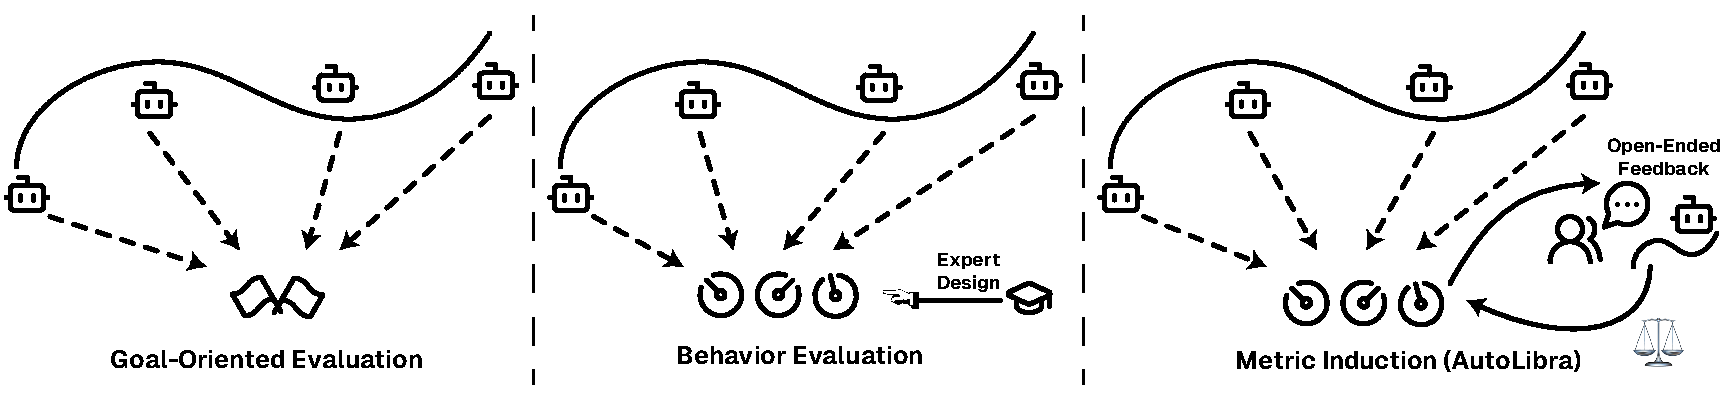
\includegraphics[width=0.45\textwidth]{figs/autolibra.pdf}
   \caption{AutoLibra provides behavioral evaluation on agent performance
    through automatic metric induction based on human feedback and agent trajectories.}
\end{wrapfigure}


Efficient human learners internalize open-ended feedback from others into self-regulation metrics
\citep{pintrich2002development,nicol2006formative}.
These metrics offer lenses for self-reflection on the
strengths and weaknesses of ourselves and ladders for self-improvement.
In this paper, we ask:
\textbf{can we automatically induce metrics to evaluate and improve language agents from natural language feedback?} 

   
The current evaluation of large language model (LLM) agents and reward modeling often fall
into two paradigms: (1) goal-oriented evaluation --
\emph{whether the agents have fulfilled the given task},
\emph{e.g.} benchmarks \citep{zhouwebarena,jimenezswe,chan2024mle,paglieri2024balrog} and reward
modeling approaches \citep{pan2024autonomous,chen2025scaling,choudhury2025process}
and (2) behavior evaluation -- \emph{how well the agents do on heuristically designed dimensions},
\emph{e.g.} social agent and human-agent interaction benchmarks \citep{zhousotopia,shao2024collaborative}
and agent failure mode analysis \citep{pan2025why,zhang2023effects,yang2023behavioral}. 
Goal-oriented evaluation is often designed to be verifiable through considering, but it is not fine-grained
or comprehensive enough to diagnose agents' behavior problems or find the bottlenecks for improvements \citep{yehudai2025survey}.  
While behavior evaluation complements it, it requires manual design of the metrics either based on top-down heuristics
\citep{zhousotopia}, or thematic analysis of the agent's behavior \citep{shao2024collaborative,pan2025why}.
This manual design process is often time-consuming and labor-intensive through expert annotations and classifications. 

In this paper, we introduce AutoLibra \protect
\includegraphics[height=1em]{figs/scale.png},
a metric induction method as a new agent evaluation paradigm 
that mitigates the limitations of the current evaluation paradigms.
This method offers behavior evaluation for agents, with the following advantages:
(1) it provides multi-dimensional behavior evaluation that is fine-grained but requires no manual design of metrics,
(2) it could be applied to different kinds of agents and tasks, and 
(3) the metrics are fully explainable and interpretable by humans.

Taking an inspiration from the code-theme steps of thematic analysis often conducted by human experts in social sciences \citep{braun2006using},
we design the Extraction process of AutoLibra as a two step process:
(1) \emph{grounding}: ground every aspect of the human feedback into a slice of the whole agent trajectory,
and (2) \emph{clustering}: cluster the aspects of all trajectories into multiple clusters of similar behaviors
that can be summarized into metrics. For example, in the context of web agents, the grounding step will
``\textsf{If you find that the button is disabled, don't click it again}'' into a slice of the agent trajectory
``\texttt{action: click[1234]} \texttt{obs: no change} \texttt{action: click[1234]}''. Similar slices where 
agents repeated interact with disabled elements could be clustered into a metric \texttt{repeated-interact-disabled}. 

The Evaluation process of AutoLibra is designed to meta-evaluate the LLM-as-a-Judge results
through matching the detected agent traits with human feedback aspects.


we design AutoLibra as a closed-loop system
that has an \emph{Extraction Step} which extracts metrics from human feedback and agent trajectories,
and an \emph{Evaluation Step} which meta-evaluates the LLM-as-a-Judge results
through matching the detected agent traits with human feedback aspects. 
Through these two steps, AutoLibra optimizes not only for metrics that represents humans' views on the
agents' behavior, but also for the metrics that are suitable for the LLM-as-a-Judge to produce human-aligned
evaluation results.

\begin{wrapfigure}{r}{0.7\textwidth}
    \centering
    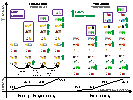
\includegraphics[width=0.7\textwidth]{figs/autolibra-teaser.pdf}
    \caption{Caption}
    \label{fig:enter-label}
\end{wrapfigure}

The Extraction Step of AutoLibra is designed to extract metrics from human feedback and agent trajectories.


With AutoLibra, we aim to answer the following research questions:
\begin{itemize}
    \item \textbf{RQ1:} Can LLMs serve as a proxy for humans when being used in agent behavior thematic analysis,
    behavior evaluation, and meta-evaluating the LLM-as-a-Judge results?
    \item \textbf{RQ2:} What are the differences between the metrics induced by AutoLibra and the behavior evaluation
    metrics designed by human experts?
    \item \textbf{RQ3:} Is AutoLibra useful for improving the performance of agents in different tasks by 
    providing fine-grained behavior evaluation for human agent engineers and agent learning algorithms?
\end{itemize}




	\section{\texorpdfstring{AutoLibra 
\includegraphics[height=1em]{figs/scale.png}}{AutoLibra}}

To address the limitations of existing evaluation paradigms, AutoLibra \protect
\includegraphics[height=1em]{figs/scale.png} is designed to
meet the following desiderata: (1) \emph{induced from agent behavior}: This ensures that metrics are grounded in agent trajectories rather than predefined by human experts, (2) \emph{self-validating}: Allows choosing minimal set of metrics that cover unseen human feedback with sufficient abstraction to be useful across different tasks, and (3) \emph{generalizable}: Applicable to various agent environments, independent of domain-specific design.

Based on feedback data collected from humans (\S\ref{sec:collecting-human-feedback}), AutoLibra achieves these desiderata through a closed-loop pipeline
consisting of two processes: \textbf{Induction Process} that converts agent behaviors and corresponding feedback into metrics, (\S\ref{sec:induction_process}) and \textbf{Evaluation Process} that predicts ratings and quality of new agent behaviors on the induced metrics (\S\ref{sec:evaluation_process}). 


\subsection{Collecting human feedback}
\label{sec:collecting-human-feedback}
In this paper, we use human feedback from two groups: (1) End-users -- for agents that interact directly with humans, we use the feedback from the users who interact and converse with the agents. CoGym \citep{shao2024collaborative}
is the environment that belongs to this category, and we use the user comments collected in their study, resulting
in 197 trajectories with feedback. (2) Experts -- for agents that
do not directly interact with humans, we use the feedback from human annotators (five authors in this paper) who observe agent trajectories. All other environments belong to this category, these being Sotopia \citep{zhousotopia}, WebArena \citep{zhouwebarena}, WebVoyager \citep{he2024webvoyager}, Baba-is-ai \citep{cloos2024babaaibreakrules}, and MiniHack \citep{samvelyan2021minihackplanetsandboxopenended}. For each trajectory, we collect only one element of feedback; feedback is given based on the complete agent trajectories.\footnote{While in theory we can leverage feedback on specific steps to achieve better feedback grounding and multiple feedback for single trajectory, we leave it as future work.}

\begin{wrapfigure}[17]{r}{0.4\linewidth}
  \vspace{-10pt}
  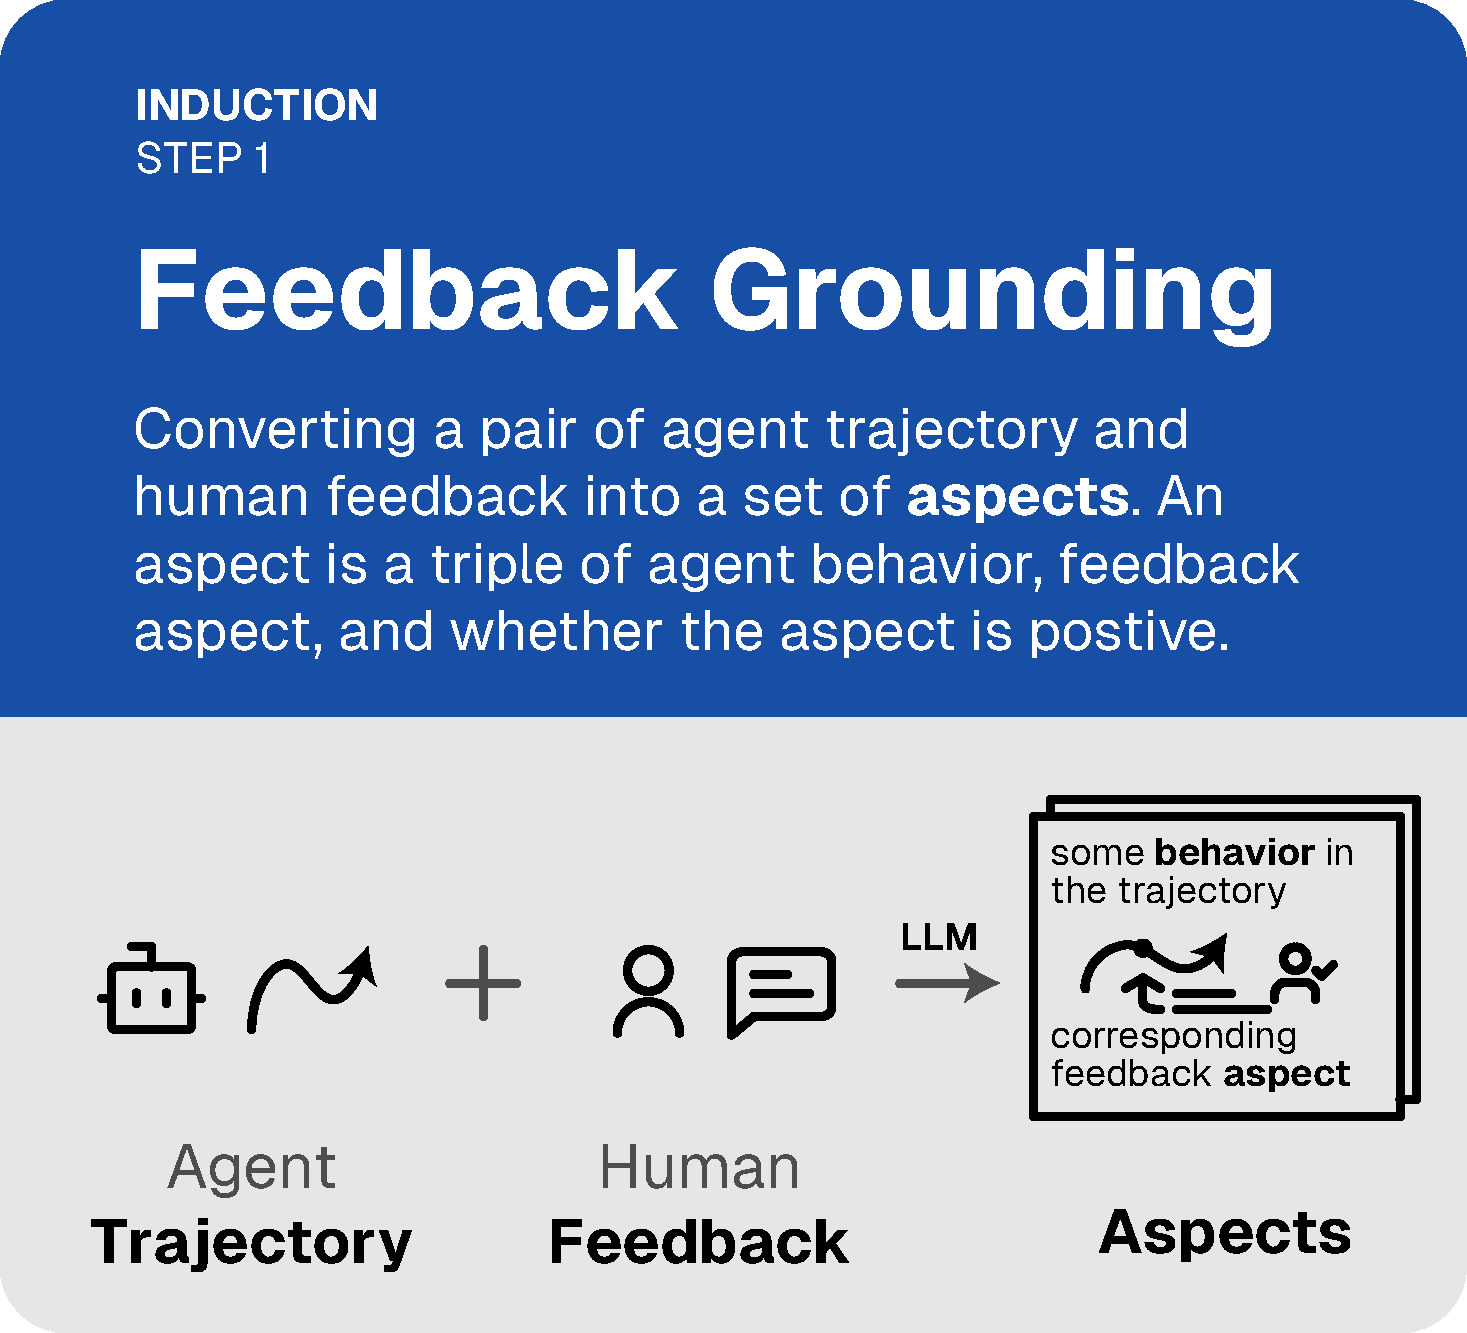
\includegraphics[width=\linewidth]{figs/autolibra_step_1.pdf}
  \vspace{-10pt}
  \caption{Feedback Grounding}
  \label{fig:feedback_grounding}
\end{wrapfigure}
Annotators are instructed to explicitly indicate the aspects of agent behavior that they classify as good or bad,
and to avoid general comments such as \textsf{"The agent is good at solving the task"}.
The annotators can also choose from a TTY (TeleTYpewriter) or a web interface; in both cases the annotator is provided with the agent's task
and then view the agent's observation and actions step by step, in text form. \footnote{While viewing screenshots is standard for web navigation tasks, we keep the observation format consistent across agents and humans to encourage more grounded feedback.}
For multi-agent tasks, we annotate each agent's trajectory in a given interaction separately. For Sotopia \citep{zhousotopia}, WebArena \citep{zhouwebarena},
and WebVoyager \citep{he2024webvoyager}, we annotate 100 trajectories of agents based on GPT-4 \citep{achiam2023gpt} with feedback for each dataset. For experiments in \S\ref{sec:ladder} we annotate 18 trajectories for each dataset in each
iteration. The annotation process is fast: Human annotators spend less than 5 minutes to provide feedback for each trajectory; \S\ref{sec:lens}, we randomly hold out 20\% of the trajectories for validation.

% \begin{figure}
%     \centering
%     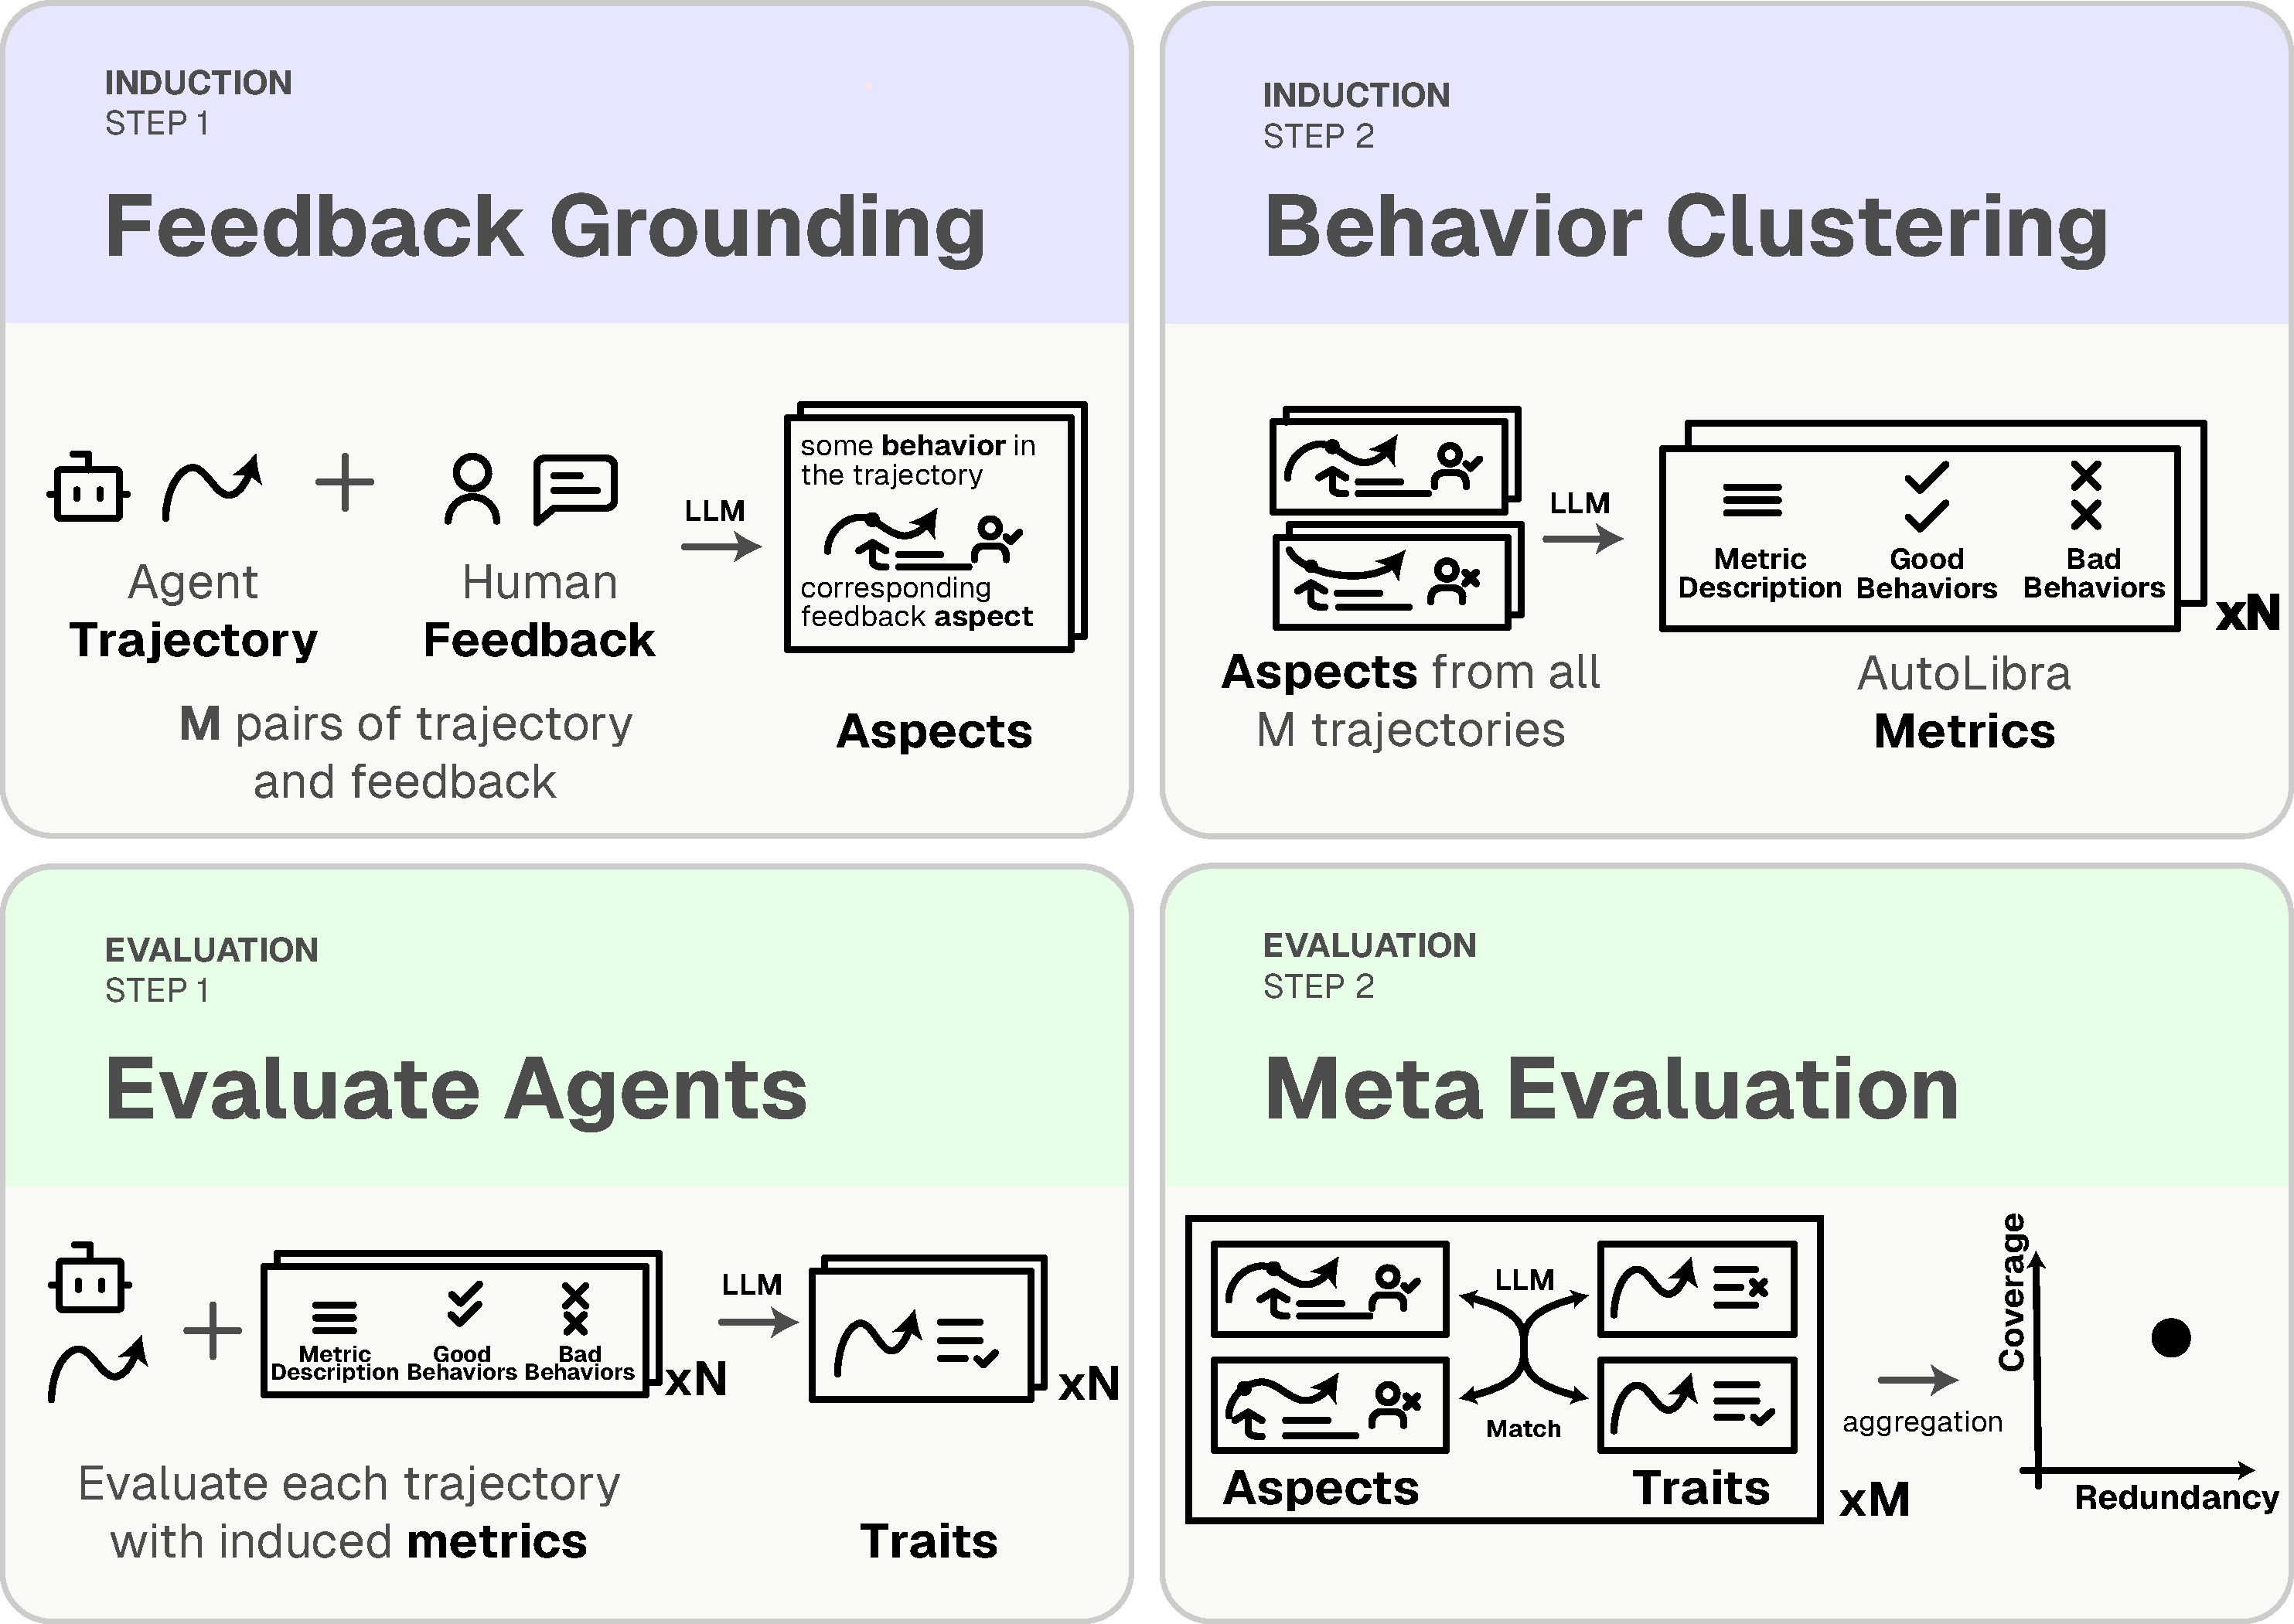
\includegraphics[width=\linewidth]{figs/autolibra_pipeline_v2.pdf}
%     \caption{Caption}
% Caption    \label{fig:enter-label}
% \end{figure}


\subsection{Induction Process: agent trajectories and human feedback $\rightarrow$ evaluation metrics}
\label{sec:induction_process}

\paragraph{Feedback Grounding}
The feedback of human annotators can contain multiple aspects; e.g. \textsf{``AI agent was pretty good
at giving me a consistent itinerary and vacation plan, although it froze on the last couple of minutes.''},
%\diyi{are all feedback from cogym? the current writeup is confusing and easily get readers to think about the feedback is from cogym only. if not, we need to add a few sentences saying how feedback is achieved, and how easy it is for humans to provide such feedback. otherwise, if this is something taking a lot of time, why do we want to use it?} 
collected from human annotators in CoGym \citep{shao2024collaborative}, contains a positive aspect
about the agent's ability to generate a consistent itinerary, and a negative aspect about the agent freezing
at the end. Here we define an \emph{aspect} as a triple $(\texttt{behavior}, \texttt{feedback}, \texttt{sign})$.
In the positive aspect of the previous example, the \texttt{behavior} is the agent's actions to create
a 20-day itinerary for the Maldives, the \texttt{feedback} is that the created itinerary is consistent and the \texttt{sign} is positive. This grounding procedure is similar to the coding procedure in thematic analysis by humans.



Illustrated in Fig. \ref{fig:feedback_grounding}, in this step, we feed the trajectory and the feedback into the LLM (we use GPT-4o \citep{openai2024gpt4ocard} 
as it yields good results in our pilot experiments) and prompt the LLM with the following instructions:
(1) break down the feedback into bullet points; (2) for each bullet point, find the corresponding
part of the trajectory to which the feedback refers. Finally, we use constrained decoding to force GPT-4o
to output the aspects in the previous format. In our experiments, we find that on most datasets, for each
trajectory, the LLM can generate one to five aspects, with a mean of one to two aspects.


\paragraph{Behavior Clustering}
\begin{wrapfigure}[16]{l}{0.4\linewidth}
  \vspace{-10pt}
  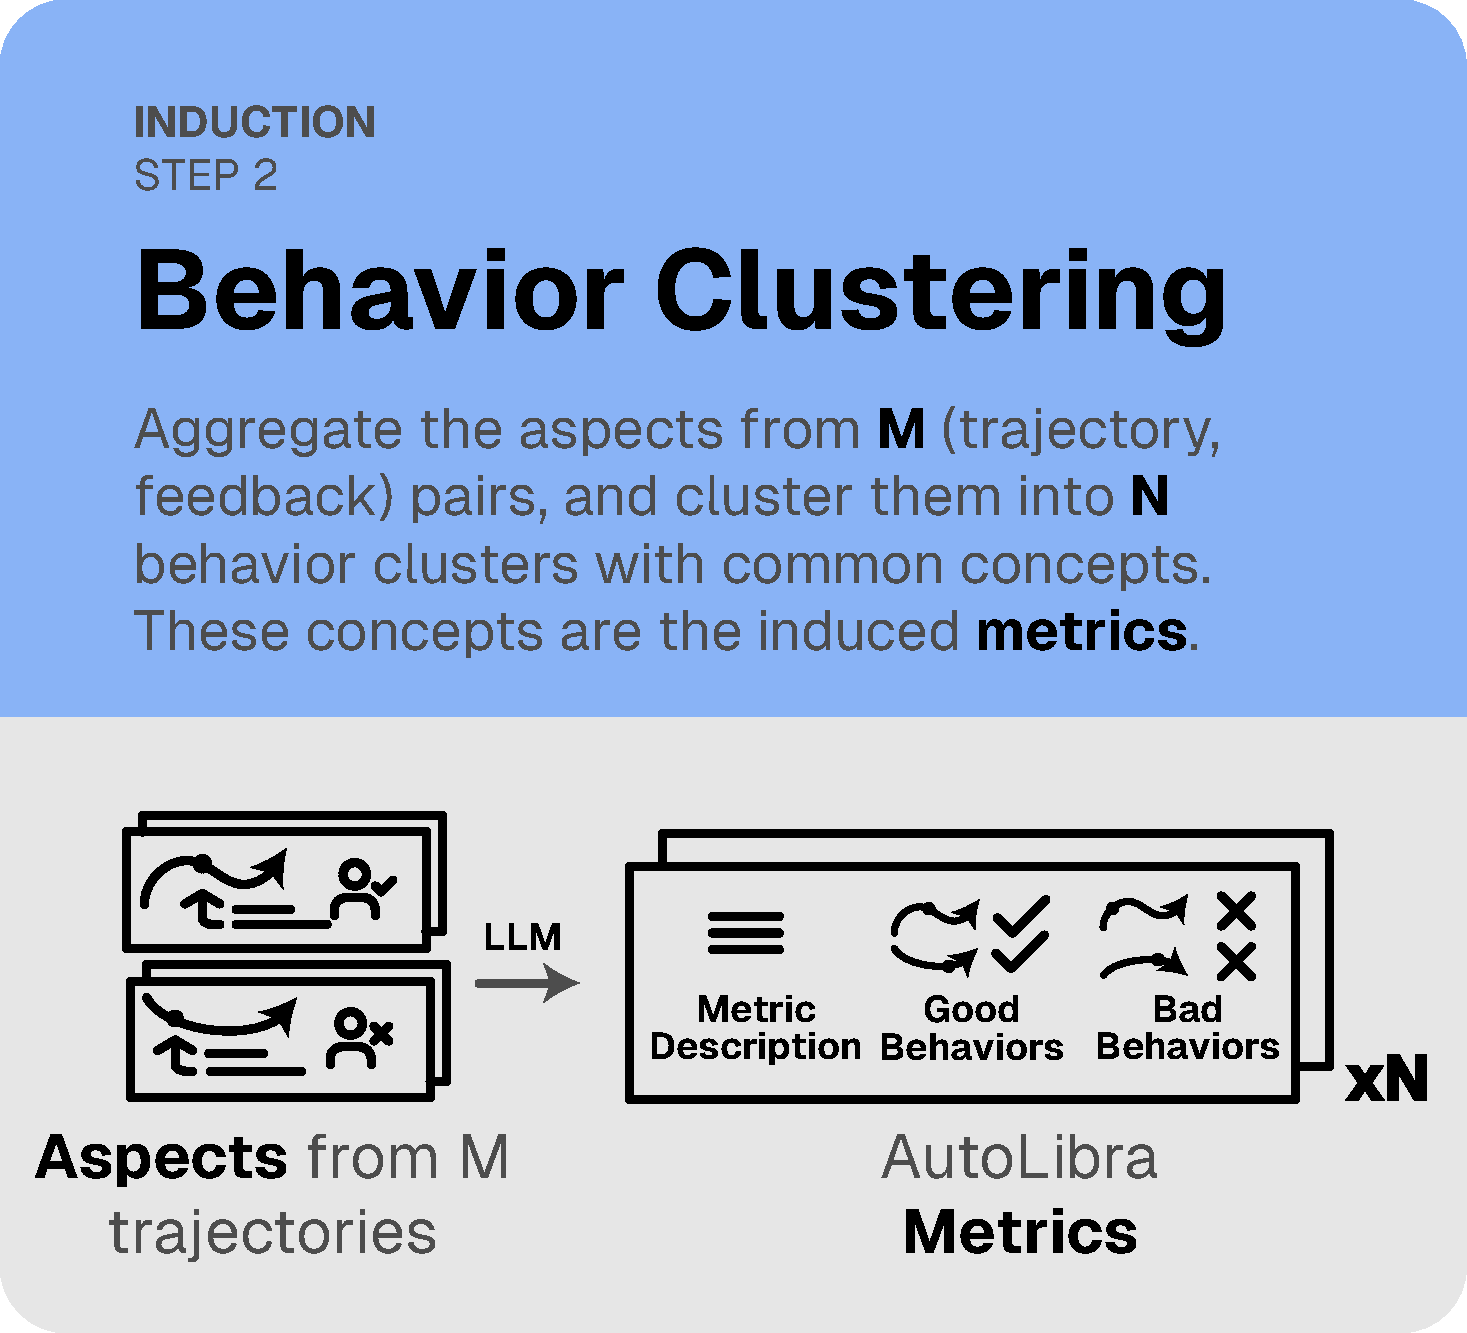
\includegraphics[width=\linewidth]{figs/autolibra_step_2.pdf}
  \vspace{-10pt}
  \caption{Behavior Clustering}
  \label{fig:behavior_clustering}
\end{wrapfigure}
The second step of the extraction process is to group the aspects into $N$ metrics.
To illustrate this step, we consider another example in the same dataset
\textsf{``The AI responds quickly to write and run the Python script``} where
the \texttt{behavior} is the agent's action to quickly write and run a Python script, the \texttt{feedback}
is that the agent responds quickly, and the \texttt{sign} is positive. Although this aspect is a positive aspect,
it reflects the same dimension of the agent's behavior as the previous negative aspect, with an opposite value.
Each \emph{metric} is a cluster of aspects, with a definition summarizing the criteria of positive behaviors, a list of positive behavior examples, and a list of negative behavior examples. This clustering procedure
is similar to the theme induction step in thematic analysis.

However, clustering similar agent behaviors together is challenging for statistical clustering methods.\footnote{
    In preliminary experiments, we tried to use K-means clustering on the aspect vectors generated by \texttt{text-embedding-3-large},
    but the clusters are mostly based on tasks and not on the behaviors.
}
Inspired by LLM-based semantic clustering and concept induction methods \citet{viswanathan2024large,lam2024concept}, we prompt an LLM (o3-mini high\footnote{https://openai.com/index/openai-o3-mini/}, as it produces the most accurate coverage and redundancy scores as evaluated later) 
to cluster the aspects into metrics. 
As illustrated in Fig. \ref{fig:behavior_clustering},
we gather all the aspects of $M$ trajectories
and cluster into $N$ metrics, where $N$ is a parameter set through the optimization process (\S\ref{sec:metric-optimization}).
We provide the LLM with the following instructions:
\emph{The granularity of the grouping should be minimal; only very similar behaviors are grouped together; but don't limit to one particular website or one particular character}, which empirically
makes the metrics more concrete but still applicable across different tasks.


\subsection{Evaluation Process: evaluating agents and the quality of the induced metrics}
\label{sec:evaluation_process}

\paragraph{Evaluating agents with induced metrics}
LLM-as-a-Judge \citep{zheng2023judging},
or more broadly, model-based evaluation
\citep{zhang2019bertscore,celikyilmaz2021evaluationtextgenerationsurvey}
is a method to use machine learning models to evaluate the output of other machine learning models.
The success of LLM-as-a-Judge depends on the gap between the difficulty of evaluation or verification and
that of generation and action. 
In agentic tasks, this gap is often large, as the policy model must perform multiple steps in decision-making, while the evaluation model must only
classify the trajectories, which make LLM-as-a-Judge widely used \citep{zhouwebarena,he2024webvoyager,zhousotopia}.
In AutoLibra, we employ LLM-as-a-Judge to
evaluate the agent trajectories configured with the induced metrics. However, LLM-as-a-Judge
can be replaced by any other evaluation methods implementing the induced metrics;
\emph{e.g.} an \texttt{interact-valid-element} metric
could be evaluated by a rule-based evaluator that checks if the agent
interacts with valid elements on the webpage. Wenote that AutoLibra could be used with other evaluation methods, such as
programmatic evaluation \citep{maeureka}; we leave generating programs for the induced metrics for future work.

\begin{wrapfigure}[16]{r}{0.4\linewidth}
  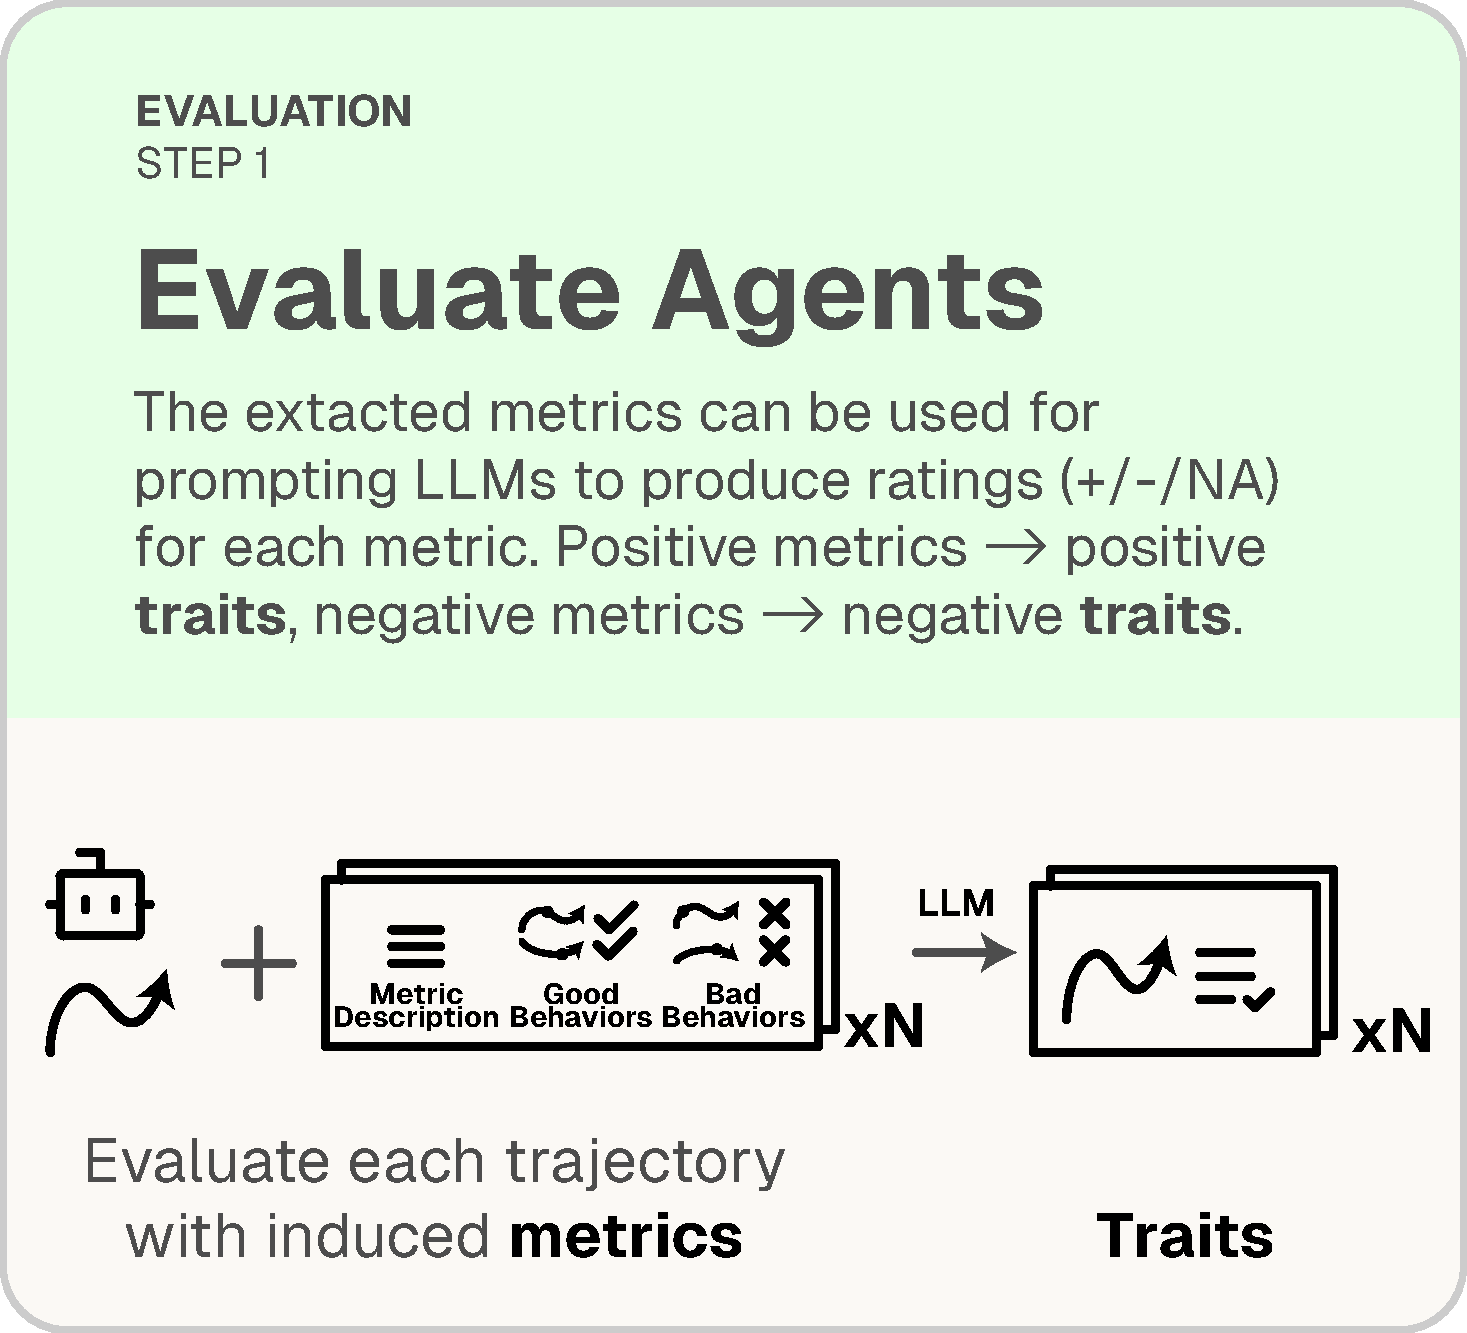
\includegraphics[width=\linewidth]{figs/autolibra_step_3.pdf}
  \vspace{-10pt}
  \caption{Evaluating agents with \\ induced metrics}
  \label{fig:llm_as_a_judge}
\end{wrapfigure}
As illustrated in Fig. \ref{fig:llm_as_a_judge}, taking the induced metrics as input, an LLM (we use o3-mini medium,
as it provides similar results in this step to o3-mini high) is prompted to rate the agent trajectories to \{+ 1, -1, N/A\} for each metric. For an agent trajectory, the metrics labeled +1 are
the positive \emph{traits}, and the ones labeled -1 are the negative \emph{traits}. When we calculate the scores of
the metrics, we use the ratio of agent trajectories rated as positive
to the ones that are rated as positive or negative, ignoring those rated as N/A,
since not all metrics are applicable to all trajectories
(some metrics like \texttt{valid-search-terms} are only applicable when the task
involves searching). 


\paragraph{Meta evaluation}
The last component of the loop is the meta-evaluation, i.e. evaluating the evaluation metrics induced by AutoLibra.
This step matches the traits detected by the LLM-as-a-Judge with aspects
grounded from the human feedback. The goal is to verify whether (1) the induced metrics cover the behaviors the human annotators care about, and (2) LLM-as-a-Judge can produce
accurate evaluation results based on the induced metrics. In the previous example,
if the \texttt{respond-promptly} is extracted as a metric, and the LLM-as-a-Judge
has the same opinion as the human annotators, then this aspect is considered as successfully covered.
If either a similar metric was not extracted, or the LLM-as-a-Judge assigns a different score,
then this aspect is considered as not covered.

\begin{wrapfigure}[15]{l}{0.4\textwidth}
  \vspace{-10pt}
  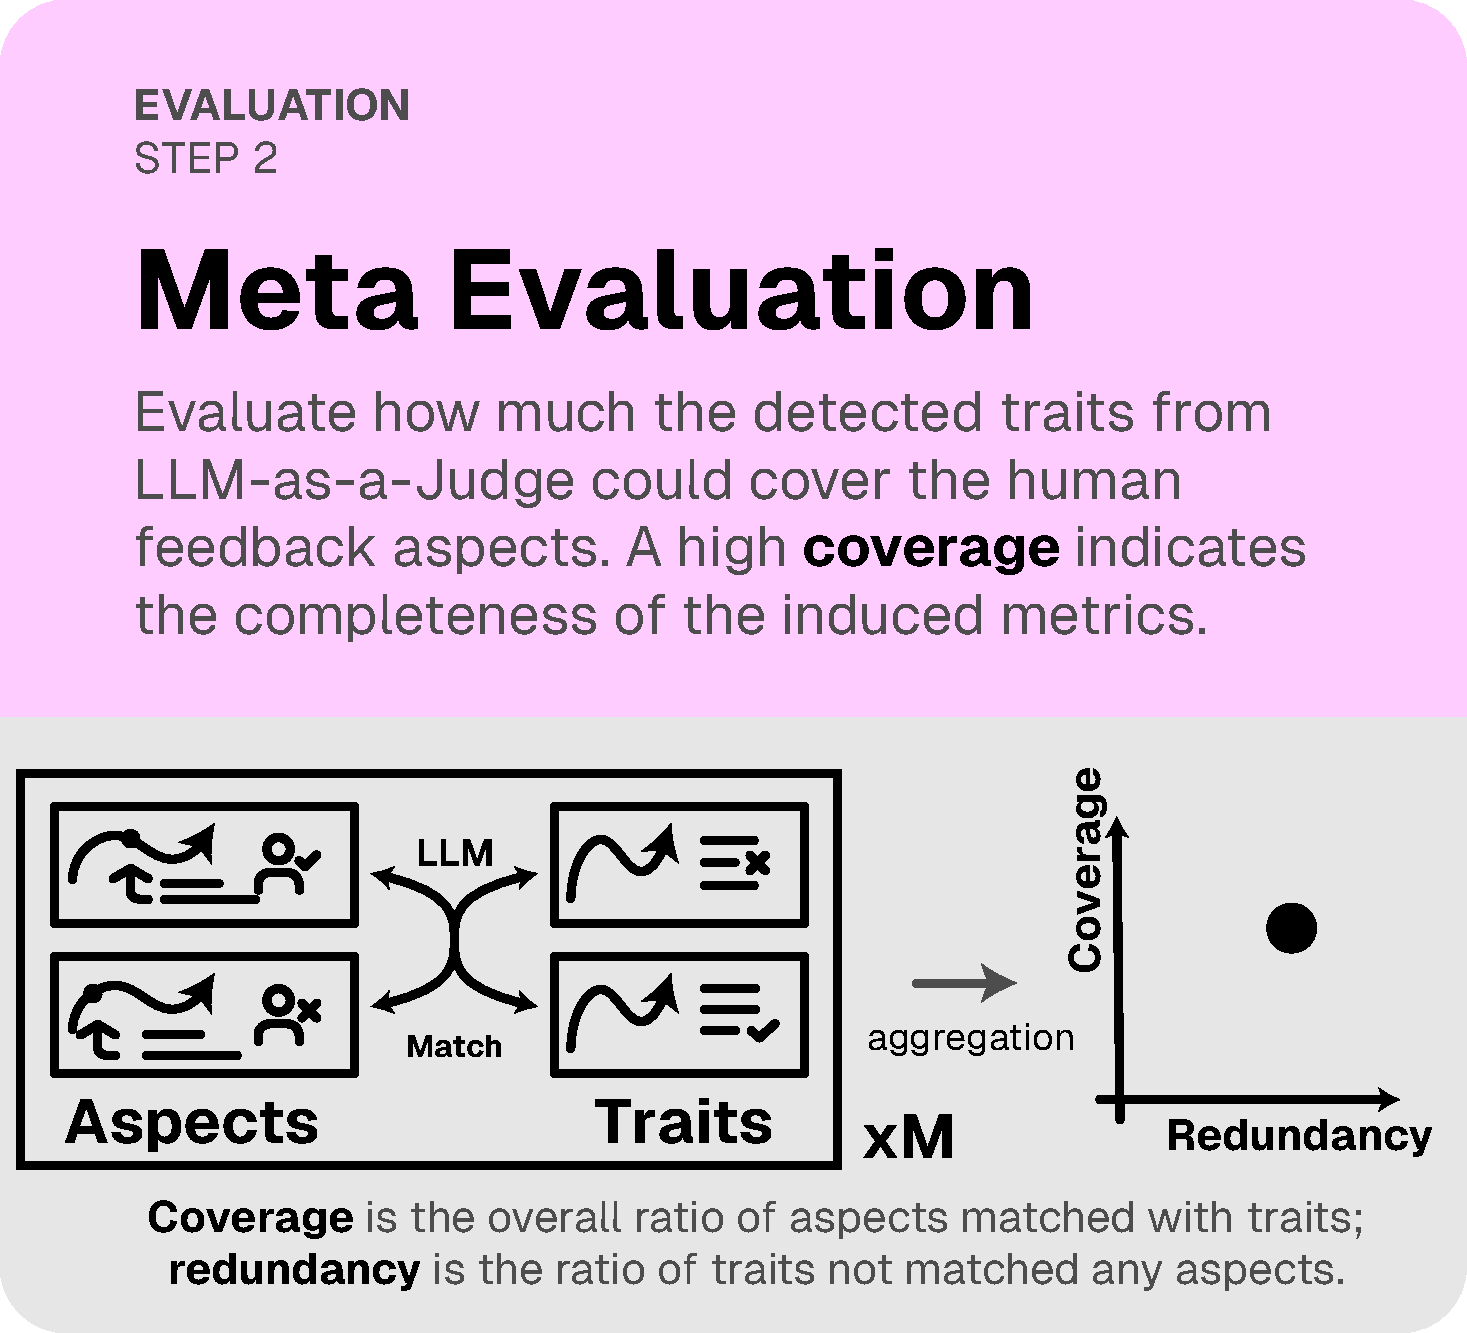
\includegraphics[width=\linewidth]{figs/autolibra_step_4.pdf}
  \vspace{-10pt}
  \caption{Meta evaluation}
  \label{fig:meta_evaluation}
\end{wrapfigure}
As illustrated in Fig. \ref{fig:meta_evaluation}, we perform meta-evaluation for each trajectory-feedback pair by classifying the aspects into positive and negative aspects, classifying
traits into positive and negative traits based on rating, then matching the positive aspects with positive traits
and the negative aspects with negative traits. 
We prompt an LLM (we use GPT-4o \citep{openai2024gpt4ocard}) with a list of aspects and another list of traits
and ask the LLM to find the best matching trait for each aspect or decide that there is no matching trait.
The \emph{coverage} of the whole dataset is calculated as the proportion of aspects of all instances that have a matching trait,
and the \emph{redundancy} is calculated as the proportion of traits of all instances that have not been matched with any aspect.

\section{Optimizing and validating AutoLibra \protect
\includegraphics[height=1em]{figs/scale.png}}
AutoLibra is designed to be self-validating through the evaluation process, which allows us to search the optimal set of metrics that cover the human opinion the best (\S\ref{sec:metric-optimization}). 
This optimization process can also be applied iteratively throughout the agent improvement process. As the agent is optimized, new metrics can be added to existing metrics (\S\ref{sec:iterative-induction}), which is similar to how unit tests are kept throughout software development to prevent new features from interfere with existing features. 
In the last part of this section, we study the alignment between each step of AutoLibra and human judgment. 


\subsection{Metric Optimization}
\label{sec:metric-optimization}

\begin{figure}[!t]
    \centering
    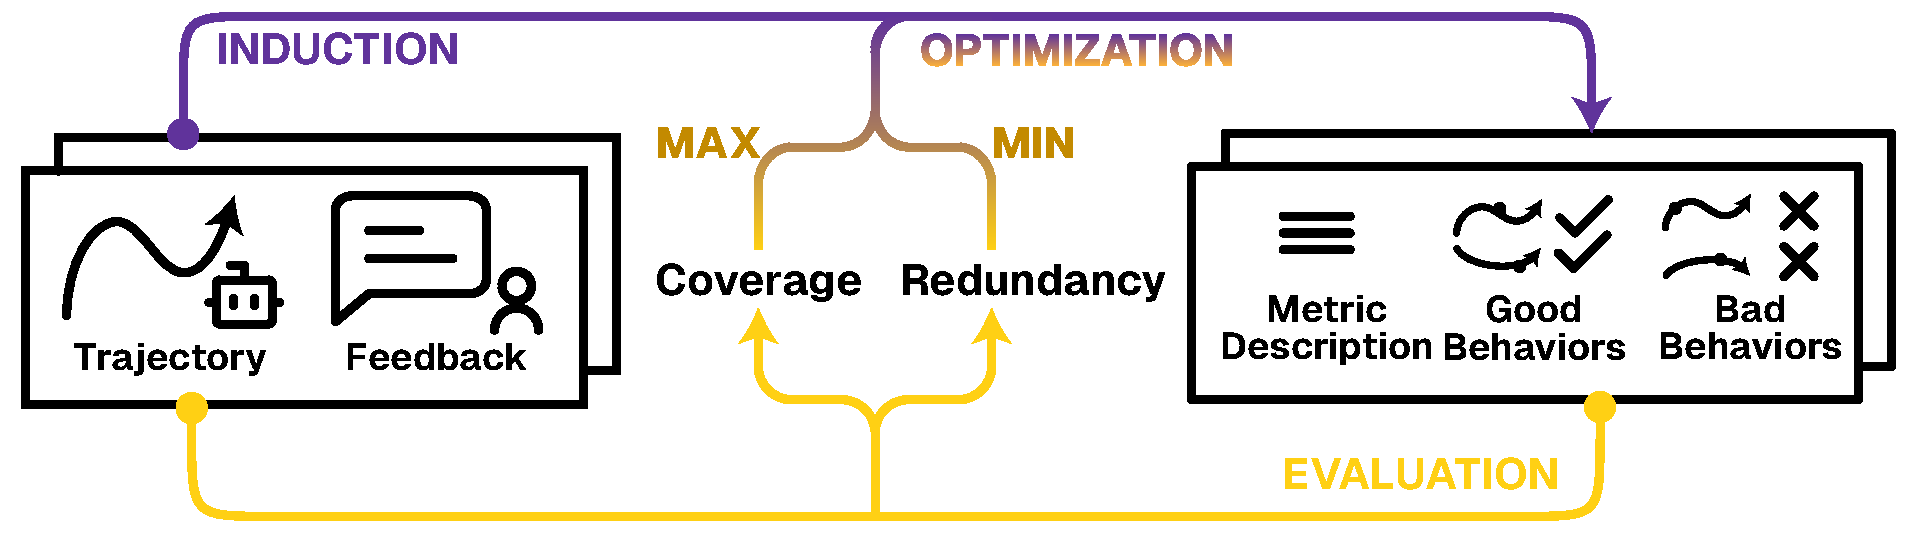
\includegraphics[width=0.8\linewidth]{figs/autolibra_optimization.pdf}
    \caption{Metric optimization: optimizing the induction process through maximizing the coverage while minimizing redundancy of the metrics, calculated via the evaluation process.}
    \label{fig:autolibra_optimization}
\end{figure}


As illustrated in Fig. \ref{fig:autolibra_optimization}, we optimize the metric induction process to maximize \textbf{coverage} and minimize \textbf{redundancy}.
Among the two, we prioritize coverage of the metrics to provide a comprehensive evaluation of the agent behavior, while minimizing overlap within the metrics to avoid redundancy, thus maximizing the utility of induced metrics.
To optimize for this objective, we generate 20 different sets of metrics, with $N$ ranging from 4 to 13,
and calculate the coverage and redundancy of the metrics in human feedback.
\begin{wrapfigure}[27]{r}{0.6\textwidth}
\vspace{-10pt}
    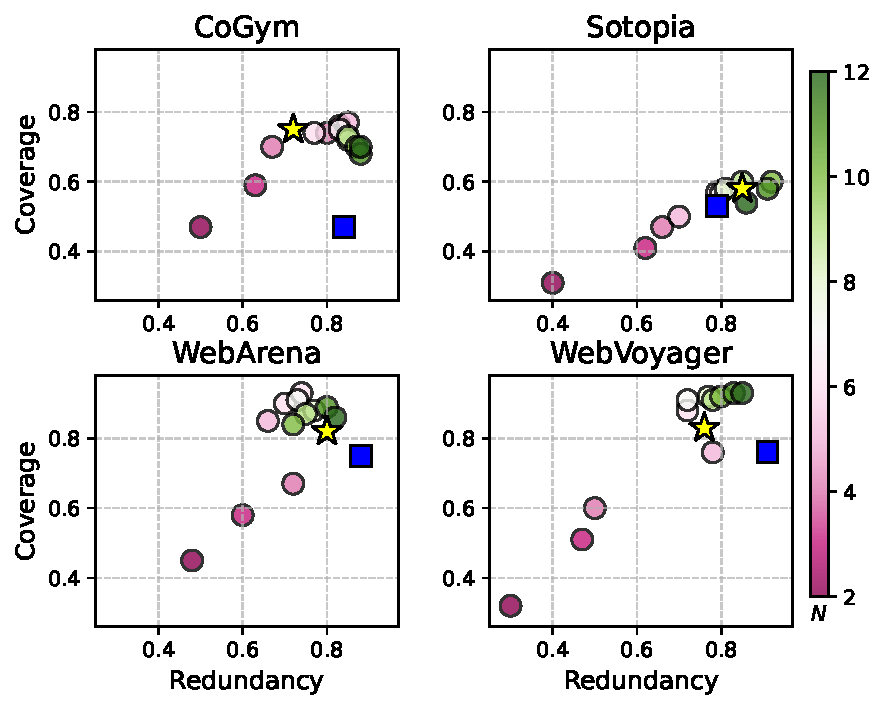
\includegraphics[width=0.6\textwidth]{figs/four_datasets_grid.pdf}
    \vspace{-15pt}  
    \caption{Coverage and redundancy of AutoLibra metrics on four agentic datasets. Circles indicate coverage and redundancy for different induced metrics; stars indicate the the best metrics' coverage and redundancy on held-out human feedback; squares show an ablation test, indicating the effect when good and bad behavior examples are removed from metrics, demonstrating the criticality of concrete behavior examples}
    \label{fig:coverage-redundancy}
\end{wrapfigure}
We then select metrics with a coverage of at least the highest coverage minus 1\%,
and the lowest redundancy.
This is performed iteratively, by resetting the range of $N$ to the number of metrics selected
previously $\pm$2, repeating until the coverage and redundancy
of the selected metrics converge, normally within 3 iterations.
While this optimization process is simple, experiments with various other optimization
strategies, including genetic algorithms and iterative clustering saw none of them
yield better results than the simple strategy.
Fig. \ref{fig:coverage-redundancy} shows the highest coverages of the metrics of size $N$, which converge around $N=6$ to $10$ depending on the datasets. The best coverage on Sotopia \citep{zhousotopia} is the lowest among all four datasets, $60\%$, likely due to the diversity of the tasks in the dataset, while coverage on WebArena \citep{zhouwebarena} and WebVoyager \citep{he2024webvoyager} are the highest, $88\%$. We also find that the coverage of the held-out trajectories is only slightly worse ($<5\%$) than the trajectories we use to induce the metrics, which is expected since we use the exact examples extracted from the latter. Lastly, we show that the good and bad behaviors are crucial in the metrics, dropping which resulting in up to $30\%$ coverage decrease (on CoGym \citep{shao2024collaborative}).



\subsection{Iterative Metric Induction}
\label{sec:iterative-induction}
When applying AutoLibra to agent optimization, we can iteratively induce new metrics, as agents develop new failure modes or new behaviors as they improve, which is useful for tracking agents' progress across different iterations.\footnote{Alternatively, a new set of metrics can be induced from scratch for each iteration -  in practice, we do not find that this results in any coverage loss, but we choose the former method for consistency} 
%For example, in the Baba-is-AI task \citep[\S\ref{sec:Baba-Is-AI}]{cloos2024babaaibreakrules}, the agent initially fails to recognize the win condition and acts randomly; after the agent improves with an in-context example in the prompt, the agent starts to follow existing win conditions, but fails to construct new win conditions. This was not mentioned in human feedback before the agent improvement, since the agent was too random to even reach the stage where constructing new win conditions is possible. Therefore, in the second iteration, a new metric \texttt{win-rule construction} should be induced to provide a new signal for further optimizing the agent.

%\diyi{did we do this, or is the below only a comment?}}

To do this, we modify the behavior clustering step, by providing the LLM with the existing metrics
and their definitions, and ask the LLM not to change the definitions of the existing metrics, 
to only add new behaviors to the existing metrics, and add new metrics if necessary.
We apply the same optimization strategy as in the metric optimization step
ensure the newly induced metrics cover emerging behaviors and do not overlap with existing metrics.

\subsection{How aligned are the steps in AutoLibra with human judgment?}
Since AutoLibra uses LLMs in each step, we first ask whether LLM outputs are reliable or aligned with human judgment. 
To measure the alignment of AutoLibra metric induction with human judgment, we validate the feedback grounding, agent evaluation, and meta evaluation steps by having human experts manually review each step (with exception of the behavior clustering step, as it is prohibitively time-intensive for human annotators to
process and cluster more than 400 aspects), scoring (1/0) based on whether they agree with the outcomes of each iteration. The coverage and redundancy scores, in combination with the validation results of the other steps in the loop, thus serve as an indirect validation for the behavior clustering step.
Table \ref{tab:validation} shows the agreement rate of human annotators in AutoLibra steps. 
It should be noted that these tasks are significantly different; e.g., grounding for WebVoyager \citep{he2024webvoyager} is challenging
due to the length and wide action space of the trajectory, and LLM-as-a-Judge for Sotopia \citep{zhousotopia} is
difficult due to the complexity of the evaluation of social interactions. Our results show that the majority (significantly over 85\%) of results in AutoLibra are reliable according to human validation. 

\begin{table}[!t]
    \centering
    \small
    \begin{tabular}{cccccc|c}
        \toprule
        Steps & CoGym & Sotopia & WebArena & WebVoyager & Baba-is-AI & Average  \\
        \midrule
        Grounding & 0.95 & 0.95 & 0.98 & 0.93 & 0.93 & 0.95 ($\pm 0.03$) \\
        LLM-as-a-Judge & 0.90 & 0.85 & 0.95 & 1.00 & 0.90 & 0.92 ($\pm 0.04$) \\
        Meta-Evaluation & 0.98 & 0.90 & 0.85 & 0.83 & 0.95 &  0.90 ($\pm 0.04$) \\
        \bottomrule
    \end{tabular}
    \caption{
        The ratio of instances marked as fully correct in human validation. For each step and each task, we randomly sample 40 instances to reach a relatively small confidence interval of $0.04$ and ask human annotators to label them as completely correct
        or not. Although the agreement scores vary across tasks and steps, the average agreement for each step and dataset is above 0.85 significantly. 
}
    \label{tab:validation}
\end{table}

%\diyi{S2 would benefit from a bit reorg. if you want, you can put 2.1, 2.2, 2.3 into one new subsection "Introducing AutoLibra (Pipeline)", and then use them as subsubsections; i would merge 2.4 and 2.5 as a second new subsection "Optimizing AutoLibra" and put the original 2.4 and 2.5 as subsubsections within it, to create more logic structures. i would move 2.6 to S3 as how you set up the initialization for using autolibra, etc.}

	\section{\texorpdfstring{AutoLibra as a lens 
\includegraphics[height=1em]{figs/microscope.png}: agent evaluation with AutoLibra}{AutoLibra as a lens: agent evaluation with AutoLibra}}
\label{sec:lens}

In this section, we use AutoLibra as a lens to provide grounded, behavior-salient insights into agent trajectories. In three data sets, CoGym \citep{shao2024collaborative}, Sotopia \citep{zhousotopia}, and WebVoyager \citep{he2024webvoyager}, we compare induced metrics with heuristically proposed evaluation dimensions and failure modes summarized by the authors. We find that AutoLibra can discover more concrete metrics than heuristically defined categories, and novel metrics that are overlooked by experts. 

\begin{table}[!h]
\centering
\begin{tabular}{ll}
    \toprule
    AutoLibra\protect
\includegraphics[height=1em]{figs/scale.png}-induced metrics & CoGym failure categories\\\midrule
    \multicolumn{2}{c}{Matched metrics and categories}\\\midrule
    \textit{Responsiveness and Efficiency} (75\%) & \textit{Communication} (65\%) \\
    \emph{Communication Clarity and Notification} (8\%) & \textit{Communication} (65\%)\\
    \textit{Instruction Adherence and Follow-Through} (24\%) & \textit{Situational Awareness} (40\%)\\
    \textit{Iterative Refinement and Adaptability} (47\%) & \textit{Planning} (39\%)\\
    \textit{Autonomy and Proactiveness} (28\%) & \textit{Planning} (39\%) \\
    \textit{Search and Retrieval Accuracy} (13\%) & \textit{Environmental Awareness} (28\%) \\
    \textit{Data Analysis Competence} (2\%) & \textit{Environmental Awareness} (28\%) \\
    \textit{Interface and User Experience} (23\%) & \textit{Personalization} (16\%) \\\midrule
    \multicolumn{2}{c}{Unmatched AutoLibra\protect
\includegraphics[height=1em]{figs/scale.png}-induced metrics}\\\midrule
     \multicolumn{2}{C{0.8\textwidth}}{\textit{Content Quality and Coherence} (16\%)} \\ \bottomrule
\end{tabular}
\caption{Comparison between AutoLibra-induced metrics and CoGym failure categories}
\label{tab:lens_cogym}
\end{table}

\paragraph{CoGym}
For CoGym \citep{shao2024collaborative}, AutoLibra induces 9 metrics from feedback from \textbf{end users}, of which 7 can be matched to the five failure categories by the CoGym authors. Both \textit{Responsiveness and Efficiency} and \textit{Content Quality and Coherence} overlap with the five failure categories. This shows that AutoLibra induces metrics that reflect human expert categorization, but also provides a different perspective to understand agent performance.

%\textit{Communication clarity and user interaction} belongs to Communication,  \textit{Adherence to instructions and consistency} belongs to Situational Awareness, \textit{Adaptability and responsiveness to feedback} belongs to Planning, \textit{Search accuracy and content relevance} belongs to Environment Awareness, and \textit{User preference query and incorporation} belongs to Personalization. All five metrics are more concrete and fine-grained than the larger categories in CoGym; we also discover the following metrics that are not mentioned in the break-down analysis in the CoGym paper:
%\textit{Responsiveness and Efficiency}, \textit{Content Quality and Coherence}, and \textit{Data Analysis Competence}. We note that this comparison shows the complementary characteristics of automatically 
%induced metrics, which are more concrete on the issues that users are noticing, while the expert-designed categories measure the high-level capabilities of AI agents. 

\begin{table}[!h]
\centering
\begin{tabular}{ll}
    \toprule
    AutoLibra\protect
\includegraphics[height=1em]{figs/scale.png}-induced metrics & Sotopia-Eval dimensions\\
    \midrule
    \multicolumn{2}{c}{Matched metrics and dimensions}\\\midrule
    \textit{Goal Achievement and Outcome Effectiveness} & \textit{Goal Completion}\\
    \textit{Conversational Naturalness and Efficiency} & \textit{Believability} \\
    \textit{Contextual Integration of Identity} & \textit{Believability}\\
    \textit{Personality Consistency and Alignment} & \textit{Believability}\\ \midrule
    \multicolumn{2}{c}{Unmatched AutoLibra\protect
\includegraphics[height=1em]{figs/scale.png}-induced metrics}\\\midrule
     \multicolumn{2}{C{0.8\textwidth}}{\textit{Negotiation Tactics and Strategic Adaptability, Clarity and Precision in Communication, Responsiveness and Conversational Termination, Adaptability and Flexibility in Dialogue}} \\ \midrule
     \multicolumn{2}{c}{Unmatched Sotopia-Eval dimensions}\\\midrule
     \multicolumn{2}{C{0.8\textwidth}}{\textit{Relationship, Knowledge, Secret, Financial and Material Benefits, Social Rules}} \\\bottomrule
\end{tabular}
\caption{Comparison between AutoLibra-induced metrics and Sotopia failure categories \diyi{should we combine Table 2 and Table 3, Table 4? }}
\label{tab:lens_sotopia}
\end{table}

\paragraph{Sotopia} In Sotopia, we \citep{zhousotopia} proposed seven dimensions for evaluating social intelligence in AI agents. With AutoLibra, we recover the exact dimension \emph{Goal Completion}, and 3 metrics as the subdimensions of \emph{Believability}, indicating that \textit{Believability} could be too high-level, while AutoLibra provides more concrete breakdown metrics. 
AutoLibra induces another four metrics which are overlooked in the heuristically proposed Sotopia-Eval dimensions. We should note that the other five dimensions in Sotopia are still valuable evaluation dimensions for social intelligence. However, behaviors captured by \emph{Financial and Material Benefits}, \emph{Knowledge}, and \emph{Secret} dimensions are often also captured by \textit{Goal Completion} and \textit{Believability}. As a result, AutoLibra produces the single \textit{Goal Achievement and Outcome Effectiveness} metric through minimizing the redundancy. Whereas, \textit{Relationship} and \textit{Social Rules} captures long-tailed behaviors which are not picked up by AutoLibra.

\begin{table}[!h]
\centering
\begin{tabular}{ll}
    \toprule
    AutoLibra\protect
\includegraphics[height=1em]{figs/scale.png}-induced metrics & WebVoyager fail reasons\\
    \midrule
    \multicolumn{2}{c}{Matched metrics and dimensions}\\\midrule
    \textit{Navigation Accuracy} (11\%) & \textit{Navigation Stuck} (44\%) \\ 
    \textit{Access Barrier Handling} (2\%) & \textit{Navigation Stuck} (44\%)\\
    \textit{Error Recovery and Iterative Adjustment} (15\%) & \textit{Navigation Stuck} (44\%)\\
    \textit{Step Efficiency and Action Redundancy} (13\%) & \textit{Navigation Stuck} (44\%)\\ 
    \textit{Information Extraction and Verification Accuracy} (16\%) & \textit{Hallucination} (22\%)\\
    \textit{Result Relevance and Problem-Specific Accuracy} (9\%) & \textit{Prompt Misalignment} (9\%)\\
    \midrule
    \multicolumn{2}{c}{Unmatched AutoLibra\protect
\includegraphics[height=1em]{figs/scale.png}-induced metrics}\\\midrule
     \multicolumn{2}{C{0.8\textwidth}}{\textit{Query and Search Strategy Efficiency} (7\%), \textit{Final Output and Summarization Quality} (18\%)} \\ \midrule
     \multicolumn{2}{c}{Unmatched WebVoyager fail reasons}\\\midrule
     \multicolumn{2}{C{0.8\textwidth}}{\textit{Visual Grounding Issue} (25\%)} \\\bottomrule
\end{tabular}
\caption{Comparison between AutoLibra-induced metrics and WebVoyager failure categories}
\label{tab:lens_wv}
\end{table}

\paragraph{WebVoyager} Similarly, for web navigation tasks, AutoLibra also discovers metrics such as \textit{Access Barrier Handling}, \textit{Error Recovery and Iterative Adjustment}, \textit{Step Efficiency and Action Redundancy} which much more closely reflect emergent agent behavior than the failure analysis categories proposed in previous work \citep{he2024webvoyager,zhou2024proposeragentevaluatorpaeautonomousskilldiscovery}, where they are often simply classified as ``navigation stuck''; full results are tabulated in Table \ref{tab:lens_wv}. This further demonstrates AutoLibra's utility in extracting behavior-salient metrics, and particularly demonstrates its ability to obtain \textbf{fine-grained metrics} that expert design would not have been able to extract. 





	\section{AutoLibra as a ladder \protect

\includegraphics[height=1em]{figs/ladder.png}
: Agent improvement with AutoLibra}
\label{sec:ladder}

% \begin{table}[!h]
% 	\centering
% 	\begin{tabular}{rcccc}
% 		\toprule        & \multicolumn{2}{c}{Baba-Is-AI (\ref{sec:Baba-Is-AI})} & \multicolumn{2}{c}{WebVoyager (\ref{sec:webvoyager})} \\
% 		                & Avg. Metrics                                          & Success Rate                                         & Avg. Metrics & Success Rate \\
% 		\midrule Iter 0 & 15.8\                                                 & 33.3                                                 & 45.9         & 34.8         \\
% 		Iter 1          & 28.2                                                  & 40.0                                                 & 53.8         & 35.5         \\
% 		Iter 2          & 40.7                                                  & 44.4                                                 & 61.3         & 38.1         \\
% 		Iter 3          & 56.7                                                  & 52.7                                                 & 69.9         & 39.7         \\
% 		\bottomrule
% 	\end{tabular}
% 	\caption{Using AutoLibra-induced metrics as optimization targets for prompt
% 	engineering and finetuning leads to improvements in the average metric
% 	positive rates (Avg. Metrics) and task success rate (Success Rate) defined by the
% 	two environments respectively.}
% 	\label{tab:baba_wv_scores}
% \end{table}


% \begin{figure}[!t]
% 	\centering
% 	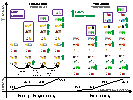
\includegraphics[width=0.8\textwidth]{figs/autolibra-teaser.pdf}
% 	\caption{AutoLibra iteratively discovers new optimization targets throughout
% 	the agent optimization process. Each emoji pair represents an induced metric;
% 	the arrows and text between iterations represents the changes made to prompts
% 	informed by metrics. Purple boxes indicate the newly emerging metrics, and
% 	green arrows indicate significant improvements over the previous iteration. The
% 	metric names can be found in Tab. \ref{tab:baba_is_ai_metrics} and App. Tab.
% 	\ref{tab:app_nnetnav_metrics}. }
% 	\label{fig:autolibra-training}
% 	\vspace{-20pt}
% \end{figure}

% \subsection{Can AutoLibra induce good optimization targets for prompt
% engineering?}
% \label{sec:Baba-Is-AI}

% To answer this question, we use \textbf{Baba-Is-AI} \citep{cloos2024babaaibreakrules, paglieri2024balrog}
% as a case study, since it is not yet saturated by state-of-the-art LLM agents. This
% game requires metacognitive skills, such as breaking and building new rules and
% planning ordered subtasks; a full list of game rules is listed in App.
% \ref{appendix:baba_is_ai_rules}. We use the top model on the leaderboard\footnote{\url{https://balrogai.com}}
% (which when we started the experiments, was GPT-4o) \citep{openai2024gpt4ocard}
% for the agent policy, while we observe similar improvements in Claude-3.5-Sonnet\footnote{\url{https://www.anthropic.com/news/claude-3-5-sonnet}}
% as well.

% % \begin{figure}[ht]
% %     \centering
% %     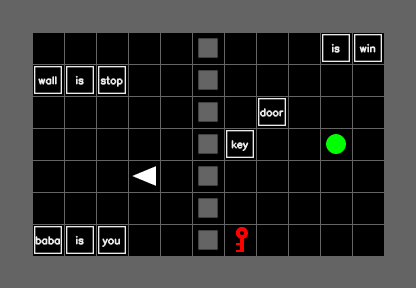
\includegraphics[scale=0.5]{figs/babaisai_env.png}
% %     \caption{Example of the Baba-Is-AI environment. In this task (two\_room-break\_stop-make\_win-distr\_obj-irrelevant\_rule), the agent has to break the "wall is stop" rule and push the "key" rule block next to "is win" to assemble the win rule, then touch the key to win. Pushing the "door" rule block would be a mistake, as no door object is present.}
% %     \label{fig:babaisai_env}
% % \end{figure}

% % \subsection{AutoLibra for Baba-Is-AI improvement}

% To avoid overfitting to the tasks used in optimization, we fine-tune on 6 of 40 tasks
% in Baba-Is-AI \citep{paglieri2024balrog}, but report performance on all 40 tasks.
% In one \textit{Iteration}, the human prompt engineers (two of the authors)
% generate 18 agent trajectories (3 trajectories / task), use AutoLibra to induce metrics,
% then optimize the prompt to achieve higher performance on the induced metrics
% without considering the task success rate, and start a new iteration when one or
% more metrics improved significantly (over 30\%). The procedure and experiment setup
% are detailed in App. Alg. \ref{appendix:algo1} and App.
% \ref{appendix:autolibra_setup}.
% \vspace{-0.4cm}

% \paragraph{Results}
% As shown in Fig. \ref{fig:autolibra-training} and Tab. \ref{tab:baba_wv_scores},
% the performance on Babaisai task increased from 25\% to 55\% between \textit{Iteration
% 0} and \textit{Iteration 3}, with each iteration resulting in greater performance
% than the previous; this is replicated across the held-out tasks alone, (complete
% task results tabulated in App. \ref{appendix:heldout}). This represents a substantial
% increase compared to the highest base model performance of 33\% on Baba-Is-AI
% \citep{paglieri2024balrog}. With only 6 tasks used in inducing the metrics, the improvement
% on all 40 tasks showing the metrics induced by AutoLibra are generalizable to unseen
% tasks. Among induced metrics (App. Tab. \ref{tab:baba_is_ai_metrics}), agent performance
% increases correspondingly to prompt changes targeting those metrics, an example
% being \texttt{Win Condition Recognition}
% 
\includegraphics[height=1em]{figs/emojis/emoji_1.png}
% , which increases from 28\% to 50\% from \textit{Iterations 0-1} after few-shot
% prompting (prompt in App. \ref{box:baba_is_you_iter_1}) is introduced to teach the
% identification of a win condition rule. The complete list of observations and
% reasoning for prompt engineering is in the App. \ref{appendix:baba_is_ai_obs}.
% With AutoLibra, prompt engineers could receive feedback on whether their prompt changes
% lead to desired behavior changes in agents.

% % \begin{wraptable}
% % 	[19]{r}{0.60\textwidth} % 'r' for right, adjust the width as needed
% % 	\centering
% % 	\small
% % 	\vspace{-10pt}
% % 	\begin{tabular}{ccl}
% % 		\toprule \multicolumn{1}{c}{Emoji}                                                & \multicolumn{1}{c}{It.} & \multicolumn{1}{l}{Metric}             \\
% % 		\midrule \rowcolor{gray!10} 
\includegraphics[scale=0.07]{figs/emojis/emoji_1.png} & 0                       & Win Condition Recognition              \\
% % 		\midrule \rowcolor{gray!10} 
\includegraphics[scale=0.07]{figs/emojis/emoji_2.png} & 0                       & Rule Modification                      \\
% % 		\midrule \rowcolor{gray!10} 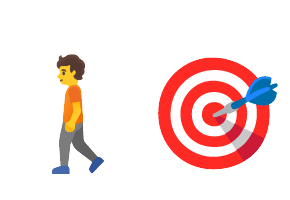
\includegraphics[scale=0.07]{figs/emojis/emoji_3.png} & 0                       & Direct Navigation Efficiency           \\
% % 		\midrule \rowcolor{gray!10} 
\includegraphics[scale=0.07]{figs/emojis/emoji_4.png} & 0                       & Context-Sensitive Decision Making      \\
% % 		\midrule \rowcolor{gray!30} 
\includegraphics[scale=0.07]{figs/emojis/emoji_5.png} & 1                       & Win Rule Construction                  \\
% % 		\midrule \rowcolor{gray!30} 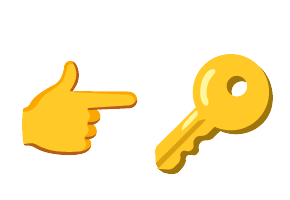
\includegraphics[scale=0.07]{figs/emojis/emoji_6.png} & 1                       & Selective Interaction w/ Relevant Obj. \\
% % 		\midrule \rowcolor{gray!30} 
\includegraphics[scale=0.07]{figs/emojis/emoji_7.png} & 1                       & Rule Manipulation and Execution        \\
% % 		\midrule \rowcolor{gray!60} 
\includegraphics[scale=0.07]{figs/emojis/emoji_8.png} & 2                       & Subtask Coordination                   \\
% % 		\midrule \rowcolor{gray!90} 
\includegraphics[scale=0.07]{figs/emojis/emoji_9.png} & 3                       & Immovable Interaction                  \\
% % 		\bottomrule
% % 	\end{tabular}
% % 	\caption{Metrics and Turn of Induction
% % 	\newline
% % 	for Baba-Is-AI}
% % 	\label{tab:baba_is_ai_metrics}
% % \end{wraptable}

% % Similarly to results observed in Section 3, induced metrics are observed to capture the behavior of the agent increasingly well with additional iterations, with coverage increasing from 65\% at \textit{Iteration 0} to 92\% at \textit{Iteration}, while mean redundancy remains 56\% across all iterations. The trajectory performance also improved significantly, with the average number of steps per task (capped at 100) decreasing from 79 to 51, indicating that the agent's reasoning performance and efficiency improved as a result of the code changes made in each iteration.

% Qualitative observation of agent trajectories reveals behaviors commensurate with
% induced metric scores; the agent random-walks in \textit{Iteration 0}, navigates
% towards specific objectives but gets stuck or trapped in a loop on long-horizon
% tasks in \textit{Iteration 1} and \textit{Iteration 2}, and fully understands basic
% subtasks (atomic goals on the critical path to environment completion) and the correct
% order of subtasks to successfully complete an environment in \textit{Iteration 3}.
% A per-metric score breakdown is listed in Appendix \ref{appendix:babaisai}, and
% a full per-iteration documentation of code changes and results is presented in
% Appendix \ref{appendix:baba_is_ai_obs}.

% % \subsubsection{Held-Out Task Performance}

% % \paragraph{Ablation Study}

% % To evaluate the generalization of the improvements realized by AutoLibra, we conducted an ablation study where the performance of the agent improved by AutoLibra was evaluated on unseen Baba Is You levels, arbitrary LLMs, and entirely new environments.

% \textbf{Generalization to other models} When replacing GPT-4o with Claude-3.5 as
% the LLM used in the agent (Appendix \ref{appendix:heldout}), performance was found
% to be similar across all iterations, with held-out task performance increasing
% by 20\% to 55\% between \textit{Iteration 0} and \textit{Iteration 3} and
% qualitatively similar trajectory performance and agent behaviors observed
% between the two LLMs. This demonstrates that the improvements realized by AutoLibra
% are generalizable to other LLMs, and that the induced metrics are robust to
% changes in the underlying LLM.

% \textbf{Generalization to other tasks} To evaluate whether this pipeline can be generalized
% to other domains, we conduct the same pipeline to MiniHack \citep{samvelyan2021minihackplanetsandboxopenended},
% an environment whose tasks and action space are more complex than Baba-Is-AI. Similarly
% to Baba-Is-AI, in three iterations, the task completion rate was observed to increase
% to 25\%, an improvement of 15\% versus the baseline of 10\%, validating
% AutoLibra's general utility in improving agent performance; full results are available
% in the Appendices \ref{appendix:minihack_rules}-\ref{appendix:minihack_obs}.
% %\diyi{use a paragraph title to illustrate that this is about generalization? i also didn't quite follow why minihack is only summarized using these two sentences. if you want to emphasize it, explain it clearly; otherwise, no need to mention it? }



% \subsection{Can AutoLibra induce good optimization targets for agent fine-tuning?}

\begin{figure}[!t]
\centering
	\vspace{-20pt}
	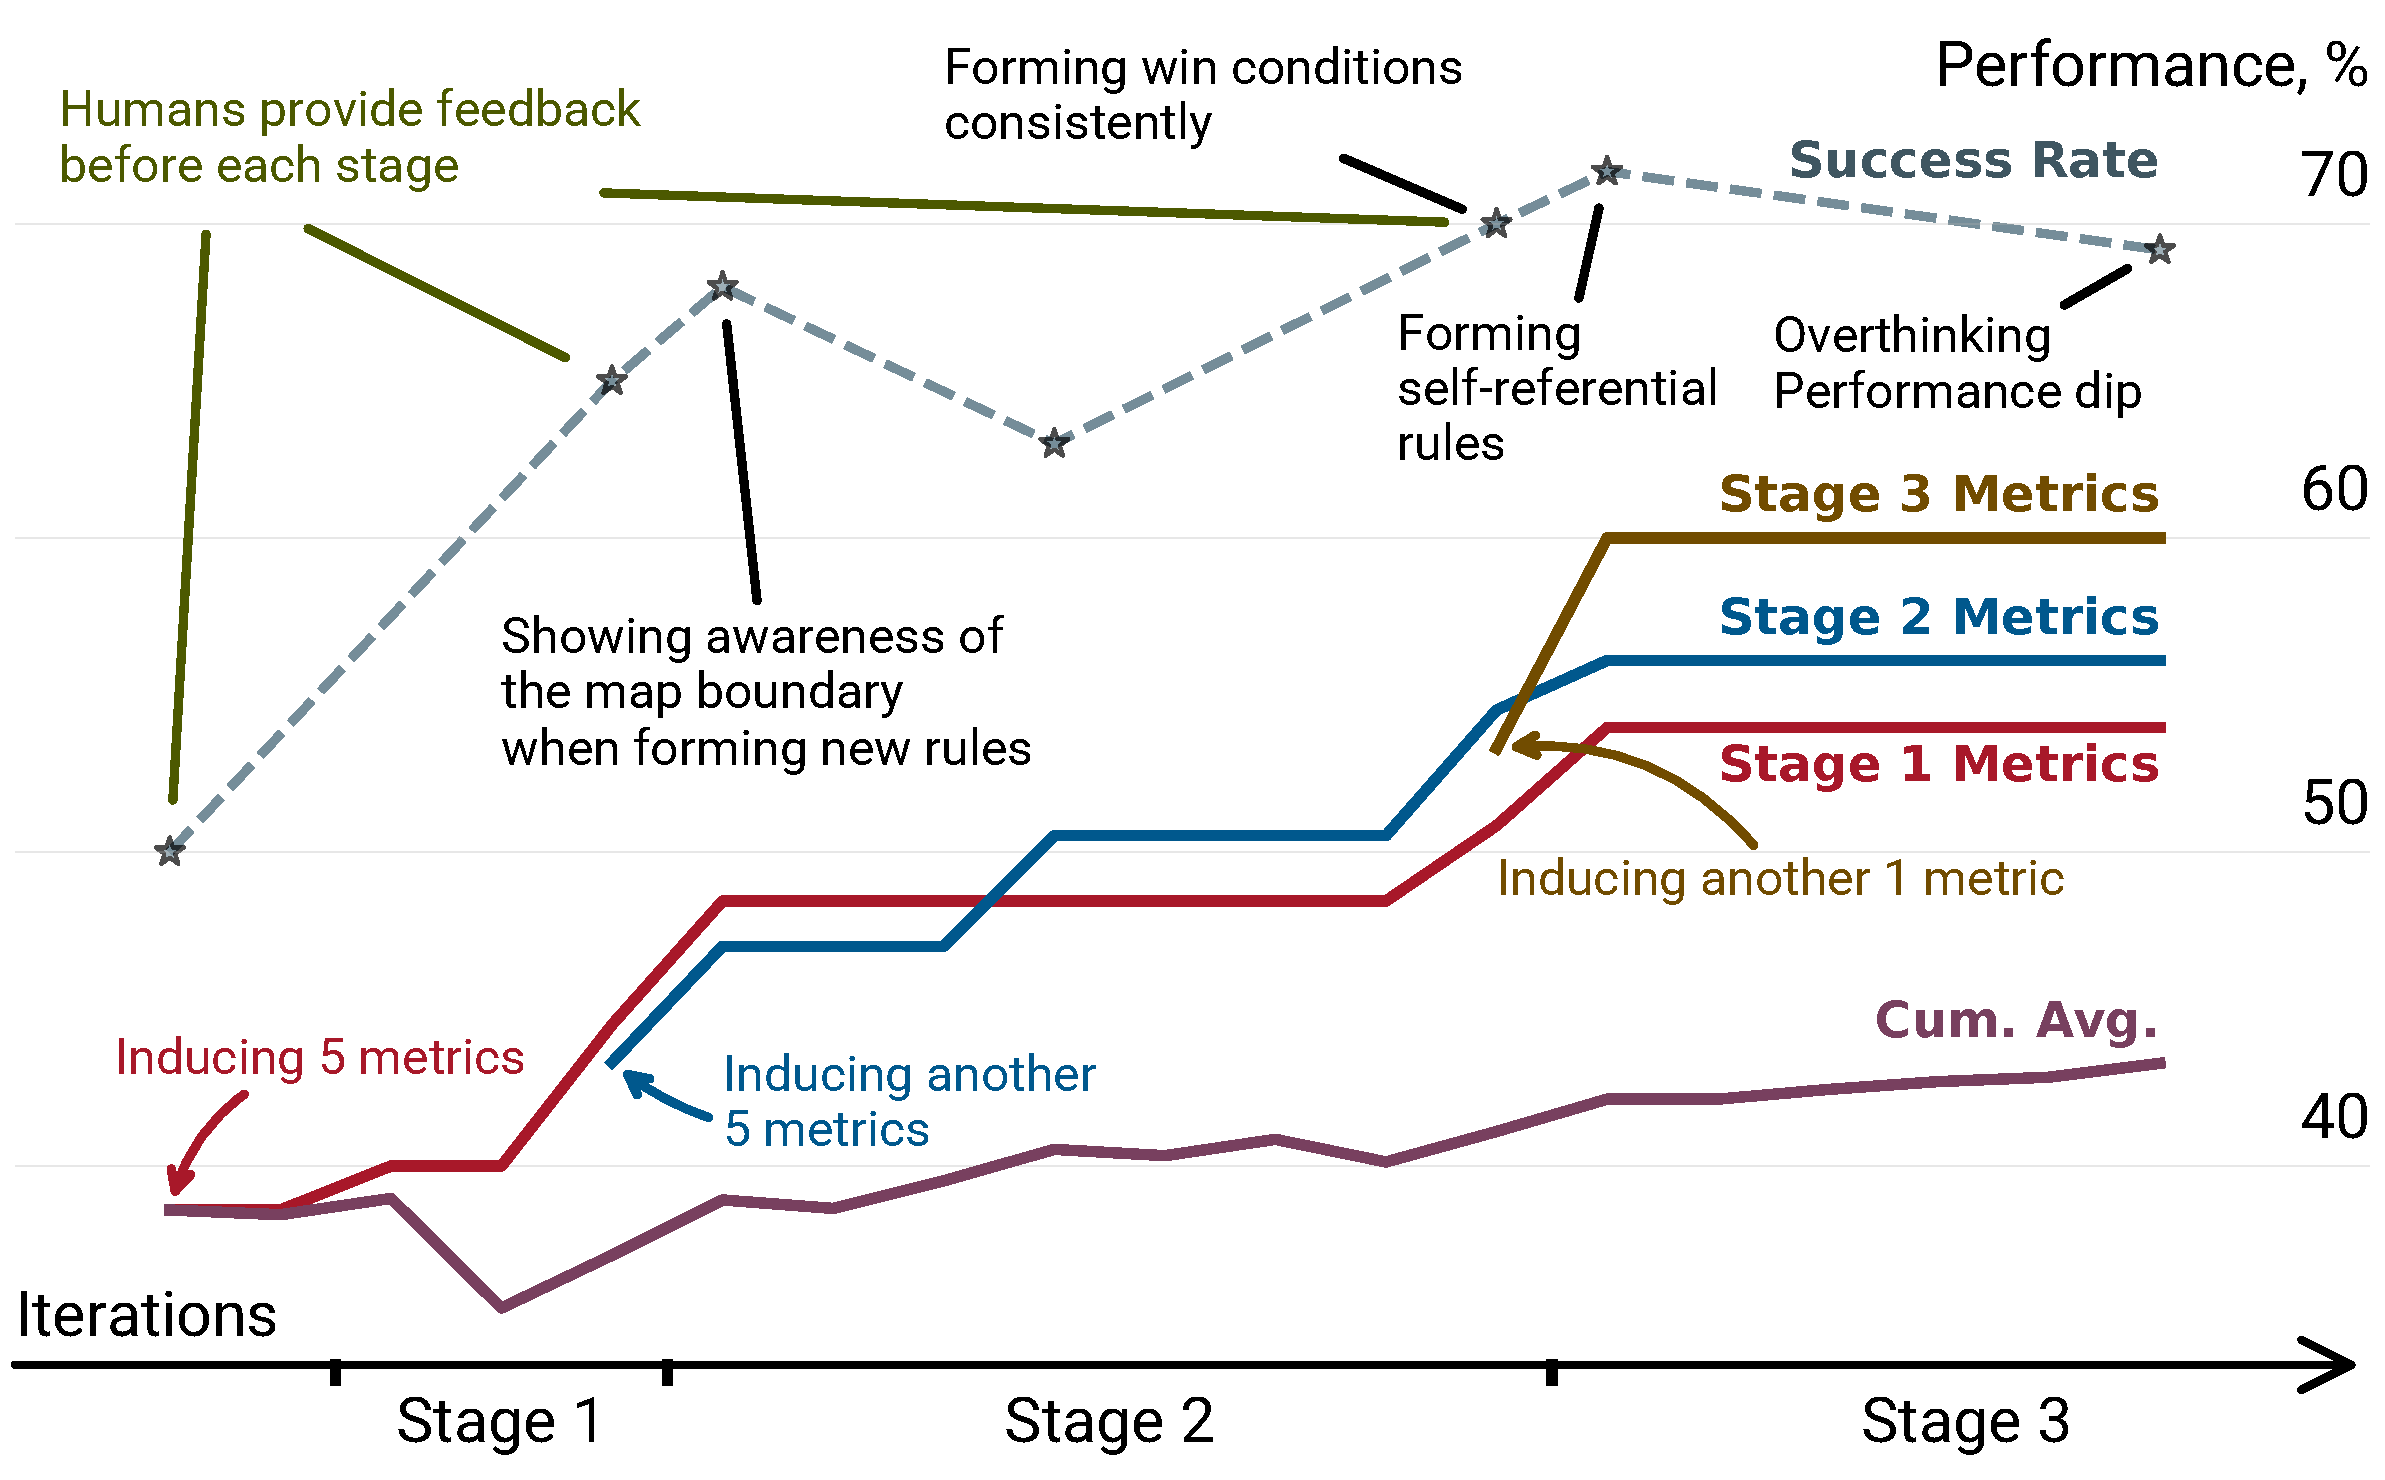
\includegraphics[width=0.8\textwidth]{figs/running_maximum_plot.pdf}
	\vspace{-15pt}
	\caption{AutoLibra iteratively induce metrics and improves the agent prompts through optimizing for the induced metrics. Although not optimized for, the success rate of the agent continuously improve until Stage 3, when the agent begins to overthink.}
	\label{fig:autolibra_self_improving}
\end{figure}


As AutoLibra can automatically induce metrics from human feedback, a natural
question to ask is whether it can enable self-regulated improvement in agents
through iterative feedback.
This can be achieved through optimizing the agent
prompts towards higher scores on the metrics extracted by AutoLibra. 
To answer this question, we use a challenging 2D game Baba-Is-AI  \citep{cloos2024babaaibreakrules, paglieri2024balrog}
as a benchmark.
Inspired by \href{https://hempuli.com/baba/}{Baba-Is-You}, this game requires not only following rules to 
achieve goals, but also manipulating the rules, 
even self-referential ones. 
For example, in the game illustrated in App. Fig. \ref{fig:baba-is-ai}, the agent needs to change self-referential rules from \textsl{baba is you}, to \textsl{door is you} to control the green door on the other side of the wall, form a new win rule \textsl{ball is win}, and navigate to the red ball to achieve the win condition.
To achieve a high score on this dataset, the agent needs not only planning, but also metacognitive skills, which is very challenging for LLM agents with frontier models as shown in the Balrog benchmark \citep{paglieri2024balrog}. In this experiment, we use Gemini-2.5-Flash \citep{geminiteam2025geminifamilyhighlycapable} for the agent, AutoLibra, and agent prompt optimization, throughout the experiment, which will be referred as the LLM in this section. Gemini-2.5-Flash is ranked as the 3rd place, with a success rate of $50.8\%\pm 4.6\%$ on the Balrog leaderboard for Baba-is-AI at the time of submission, and the state-of-the-art result is $56.7\%\pm4.5\%$.

Fig. \ref{fig:autolibra_self_improving} illustrated our procedure, and summarized the results. 
We employ an iterative process by improving the agents in 3 stages through providing human feedback on 6 out of 40 tasks in the Baba-Is-AI. Before each stage we show human annotators 3 trajectories for the 6 tasks, gather the feedback, and apply AutoLibra iterative metric induction process (\S\ref{sec:iterative-induction}). This results in 5 metrics for Stage 1 and 2, and another 1 metric for Stage 3. 
Within each stage, we iteratively feed 1 LLM agent trajectory on each of these 6 tasks, together with evaluation results based on these AutoLibra-induced metrics to the LLM to improve the prompt of the LLM agent. 
This process results in continuous improvement not only on the running maximum metric scores, the cumulative average metrics, but also game success rate. Fig. \ref{fig:autolibra_self_improving} shows these statistics on the whole 40 tasks, although we only use 6 out of the 40 tasks in the whole optimization process. 
Upon examining the agent trajectories, we find the 
skills learned in the process. In the first stage, the agent learns to find rules to form based on the map boundary, which could be a result of an induced metric \texttt{map-n-constraint-recognition}.
Similarly, more advanced skills are learned in Stage 2 and 3, including forming win conditions and self-referential rules, probably as a result of metric \texttt{rule-manipulation-proficiency}.

Our results show that the metrics induced by AutoLibra form effective objectives for improving the agents through prompt optimization. It should note that AutoLibra is a metric induction method, which is orthogonal to learning algorithms, including prompt optimization, fine-tuning or reinforcement learning. We show that this process improves agent success rate by 20\% without optimizing for success rate, and in the future, researchers can study the effect of employing other learning algorithm. 
	\section{Related Work}
AutoLibra unifies three areas of research: it draws inspiration from \textit{thematic analysis} to create \textit{nautral language-derived evaluation metrics} to evaluate and reward \textit{AI agents}. 

\paragraph{Evaluating AI agents} Much of the work in AI agent evaluation focuses around benchmarks which contains both task suites and evaluation metrics. In addition to the datasets we used in this paper, SWE-Bench \citep{jimenezswe} uses human-written unit tests as evaluation metrics; Embodied Agent Interface \citep{li2024embodied} provides fine-grained evaluation for LLM-based embodied agents; $\tau$-Bench \citep{yao2024tau} compares database states for evaluation; concurrent work AgentRewardBench \citep{lù2025agentrewardbenchevaluatingautomaticevaluations} builds a benchmark for reward models for web agents. Recently, there are observatory tools including Galileo \citep{galileo_agentic}, Vertex AI Gen AI \citep{google_agent_eval}, and Docent \citep{meng2025docent} which provide user interfaces to visualize agent failure modes. Generating intrinsic rewards have also been studied in the reinforcement learning community \citep{du2019liir,pathakICMl17curiosity,laskin2022cic} to encourage exploration, sub-task completion, or skill discovery. In contrast to these, AutoLibra is a pure data-driven task-agnostic method without predefined failure taxonomy for generating interpretable metrics for agents. 

\paragraph{Learning from natural language and human feedback} Researchers have been studying reinforcement learning with language feedback to provide a dense reward to agents \citep{goyal2019using}. Since LLM agents are even harder to train with sparse reward, there is substantial interest in training LLM agents from natural language feedback. \citet{chen2024learning} propose an imitation learning method for learning from human feedback; Text2Reward \citep{xietext2reward} uses code generation to generate robot reward functions from open-ended human feedback; our work \citep{chen2025fine} uses feedback to the improvement agent policy with prompting and then align the unprompted agent policy with the prompted one; \citet{shi2024yell} propose a new model architecture to incorporate human feedback into policy learning. On the other hand, human non-open-ended feedback is also incorporated in training agents, including rating feedback \citep{nguyen2017reinforcement}, preference feedback \citep{christiano2017deep}, demonstrative feedback \citep{shaikhaligning}.
Unlike these papers, AutoLibra induces metrics from feedback from all annotated instances and generates metrics that are generalizable to different tasks and useful for both evaluation and agent fine-tuning.

\paragraph{Automatic thematic analysis} Thematic analysis is a powerful tool for qualitative study through coding and iterative creation of themes. \citet{gauthier2022computational} provide computational tools to aid this process; \citet{hong2022scholastic} and \citet{gebreegziabher2023patat} explore human-AI collaboration in thematic analysis; LLooM \citep{lam2024concept}, is an automatic method for concept induction, is closest to and influences our approach. This paper completes the loop of concept induction by using the meta-evaluation step to optimize the induced metrics, and apply this social science technique to agent evaluation. 
	\section{Conclusion and Future Work}
This work introduces AutoLibra, a new paradigm for agent evaluation, one of
the first works to explore adaptable trajectory-derived evaluation heuristics,
offering substantial advantages in agent training over traditional end-to-end
evaluation. We find that this framework is generalizable to a diverse range of agent
tasks, provides new insights into agent behaviors, and identifies strong optimization
targets for agent improvement. There are a few directions for further extending
and applying this framework.
(1) \textbf{Behavior-centric evaluation} AutoLibra leads a \emph{paradigm shift}
from end-to-end agent evaluation (analogous to ``integration tests'' in software
development) to evaluation with granular metrics that measure agents' concrete behaviors
(analogous to ``unit tests''). Future work can study whether this process can be
improved through better human-AI collaboration.
(2) \textbf{Sub-trajectory feedback from humans} In AutoLibra, we label each
trajectory with one piece of feedback, and ground it into the agents' concrete
behavior which is at the sub-trajectory level. In the future, researchers can
let users directly give feedback for one or multiple steps in the trajectory, which
should lead to better feedback grounding results. Similarly, user feedback can be
collected during the interaction instead of after the agent has completed the tasks,
which is a more user-friendly way to gather high quality feedback data.
(3) \textbf{Wider exploration of agent improvement methods} In this paper, we only
explored non-parametric for agent improvement to show the utility of AutoLibra. Future work can use AutoLibra to provide dense rewards for individual
steps, and use reinforcement learning to train agents with these dense rewards.

	\section*{Ethics Statement}
	This research adheres to the ICLR Code of Ethics.
    Within human-aided experiments,
	we are also limited by the diversity of human annotators. The annotation of the data in this paper,
    are performed through objective and blinded surveys filled out by the authors
    who do not know which models that they are annotating.
    The human feedback for CoGym \citep{shao2024collaborative}
    is published by the original authors.
    Since the annotations are objective surveys on the performance of the agents
    without any harm to the authors or personal information gathered, this is exempted from IRB review based on the policy
    of authors' institution.
    \section*{Reproducibility Statement}
To ensure reproducibility of our results, we provide comprehensive documentation of our experimental setup and methodology in the appendix of our work. All experimental details, including
model configurations, prompting strategies, and evaluation metrics, are specified in the relevant sections and supplementary materials. All code and data will be available upon acceptance. 

	% \section*{Author Contributions}

	% \section*{Acknowledgments}
	% This work is supported by ONR grant N000142412532, and NSF grant IIS-2247357, and DARPA grant Friction for Accountability in Conversational Transactions.
	% We thank Google Cloud Platform and Modal Platform for their credits. We thank Yutong
	% Zhang, Hayley Zhang, Yijia Shao, Michelle S Lam, Manling Li, Ryan Louie, Yanzhe
	% Zhang, Xuhui Zhou, Maarten Sap, Sherry Tongshuang Wu, Shikhar Murty, Saujas
	% Vaduguru, Chenghao Yang, Xizhi Xiao, Anant Sinha and all members of Stanford SALT
	% Lab for their help and feedback throughout this project.

	\bibliography{main}
\bibliographystyle{iclr2026_conference}


	\newpage
	\appendix
	\section*{Appendix}
	\documentclass[../main.tex]{subfiles}

\begin{document}
    \section*{Content of Appendix}
    \begin{itemize}
        \item[\textbf{1.}] \textbf{AutoLibra Ladder Methodology}
            \begin{itemize}
                \item \ref{appendix:illustrations} Illustration of AutoLibra Method

                \item \ref{appendix:algo1} Algorithm of AutoLibra Ladder

                \item \ref{appendix:autolibra_setup} AutoLibra Ladder Experiment
                    Configuration
            \end{itemize}

        \item[\textbf{2.}] \textbf{Baba-is-ai}
            \begin{itemize}
                \item \ref{appendix:baba_is_ai_rules} Rules and Environment Details

                \item \ref{appendix:heldout} Experiment Results

                \item \ref{appendix:babaisai} Metric Scores

                \item \ref{appendix:babaisai_metrics} Metric Examples

                \item \ref{appendix:babaisai_prompts} Prompts

                \item \ref{appendix:baba_is_ai_obs} Qualitative Observations of Agent
                    Performance
            \end{itemize}

        \item[\textbf{3.}] \textbf{MiniHack}
            \begin{itemize}
                \item \ref{appendix:minihack_rules} Rules and Environment Details

                \item \ref{appendix:heldout_mini} Experiment Results

                \item \ref{appendix:minihack} Metric Scores

                \item \ref{appendix:minihack_metrics} Metric Examples

                \item \ref{appendix:minihack_prompts} Prompts

                \item \ref{appendix:minihack_obs} Qualitative Observations of Agent
                    Performance
            \end{itemize}

        \item[\textbf{4.}] \textbf{WebVoyager}
            \begin{itemize}
                %\item \ref{} Rules and Environment Details

                \item \ref{appendix:nnetnav_live} NNetNav-Live Induced Metrics
            \end{itemize}
    \end{itemize}

    \newpage
    \section{Illustration of AutoLibra Method}
    \label{appendix:illustrations}
    \begin{figure}[!h]
        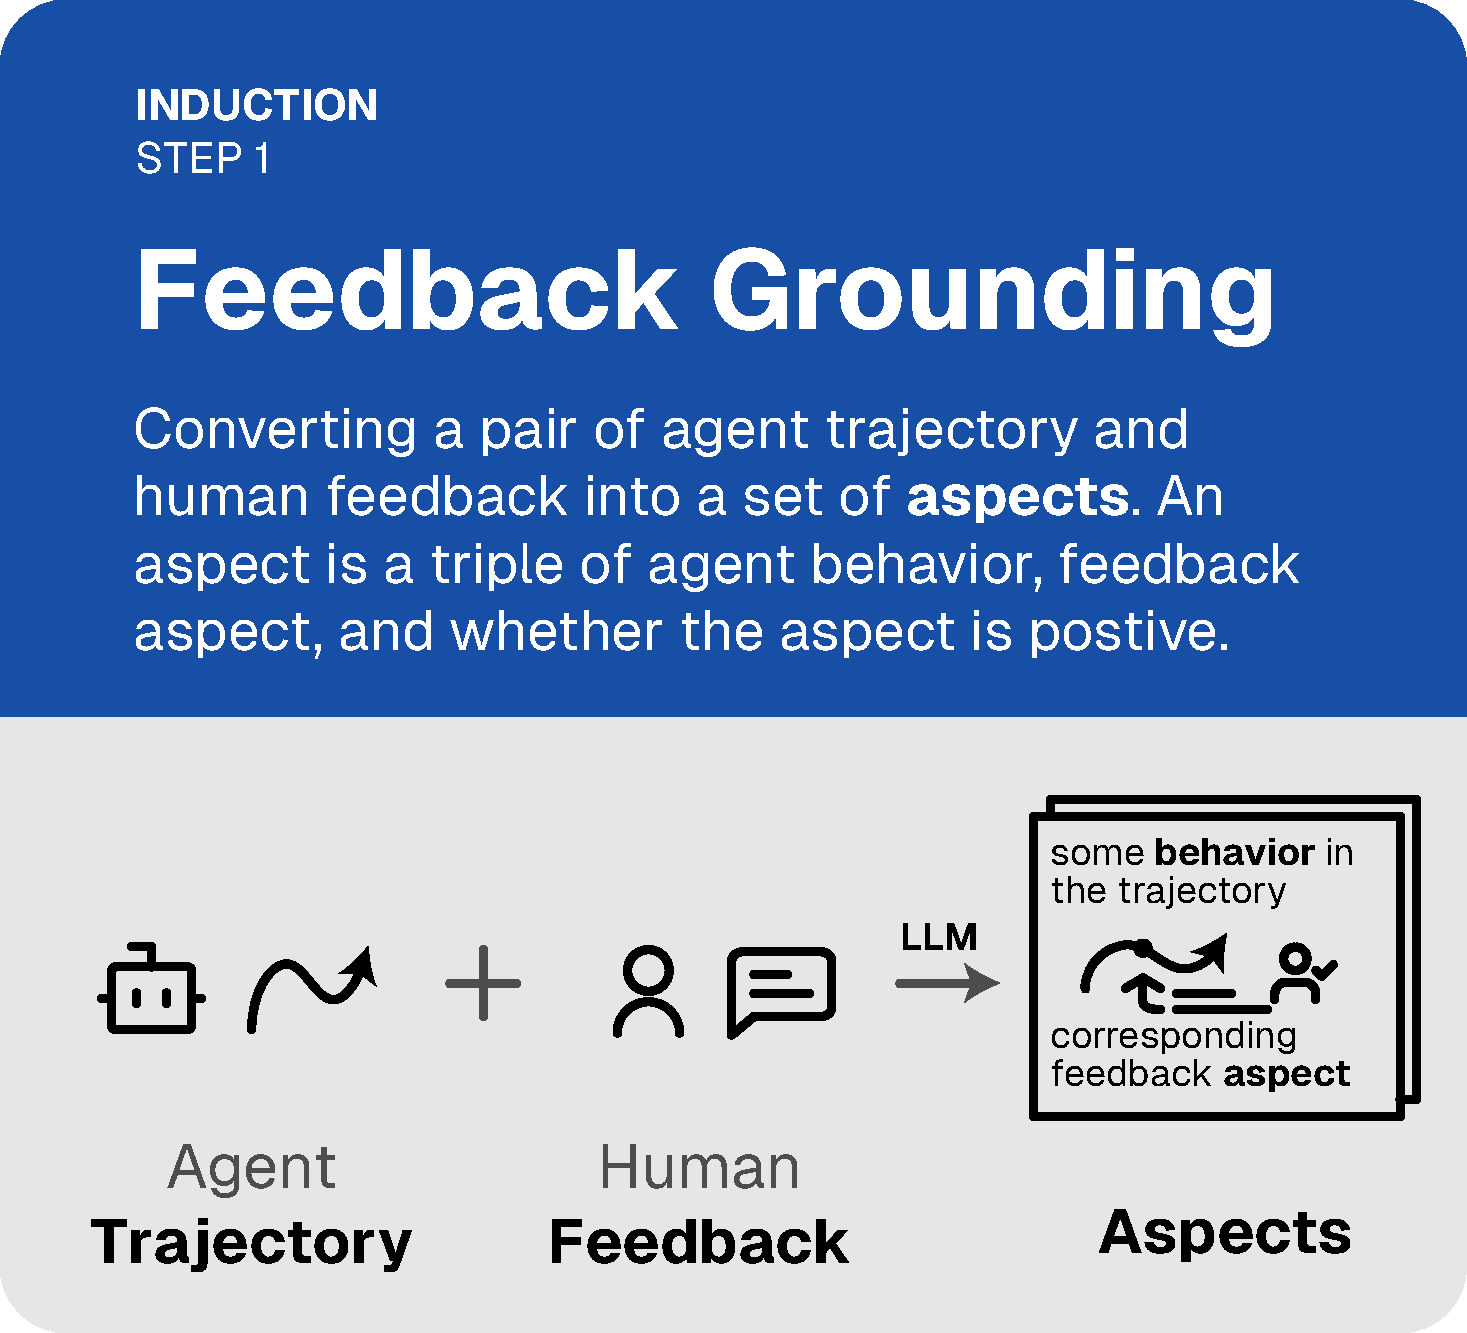
\includegraphics[width=0.4\linewidth]{figs/autolibra_step_1.pdf}
        \caption{Feedback Grounding}
        \label{fig:feedback_grounding}
    \end{figure}

    \begin{figure}[!h]
        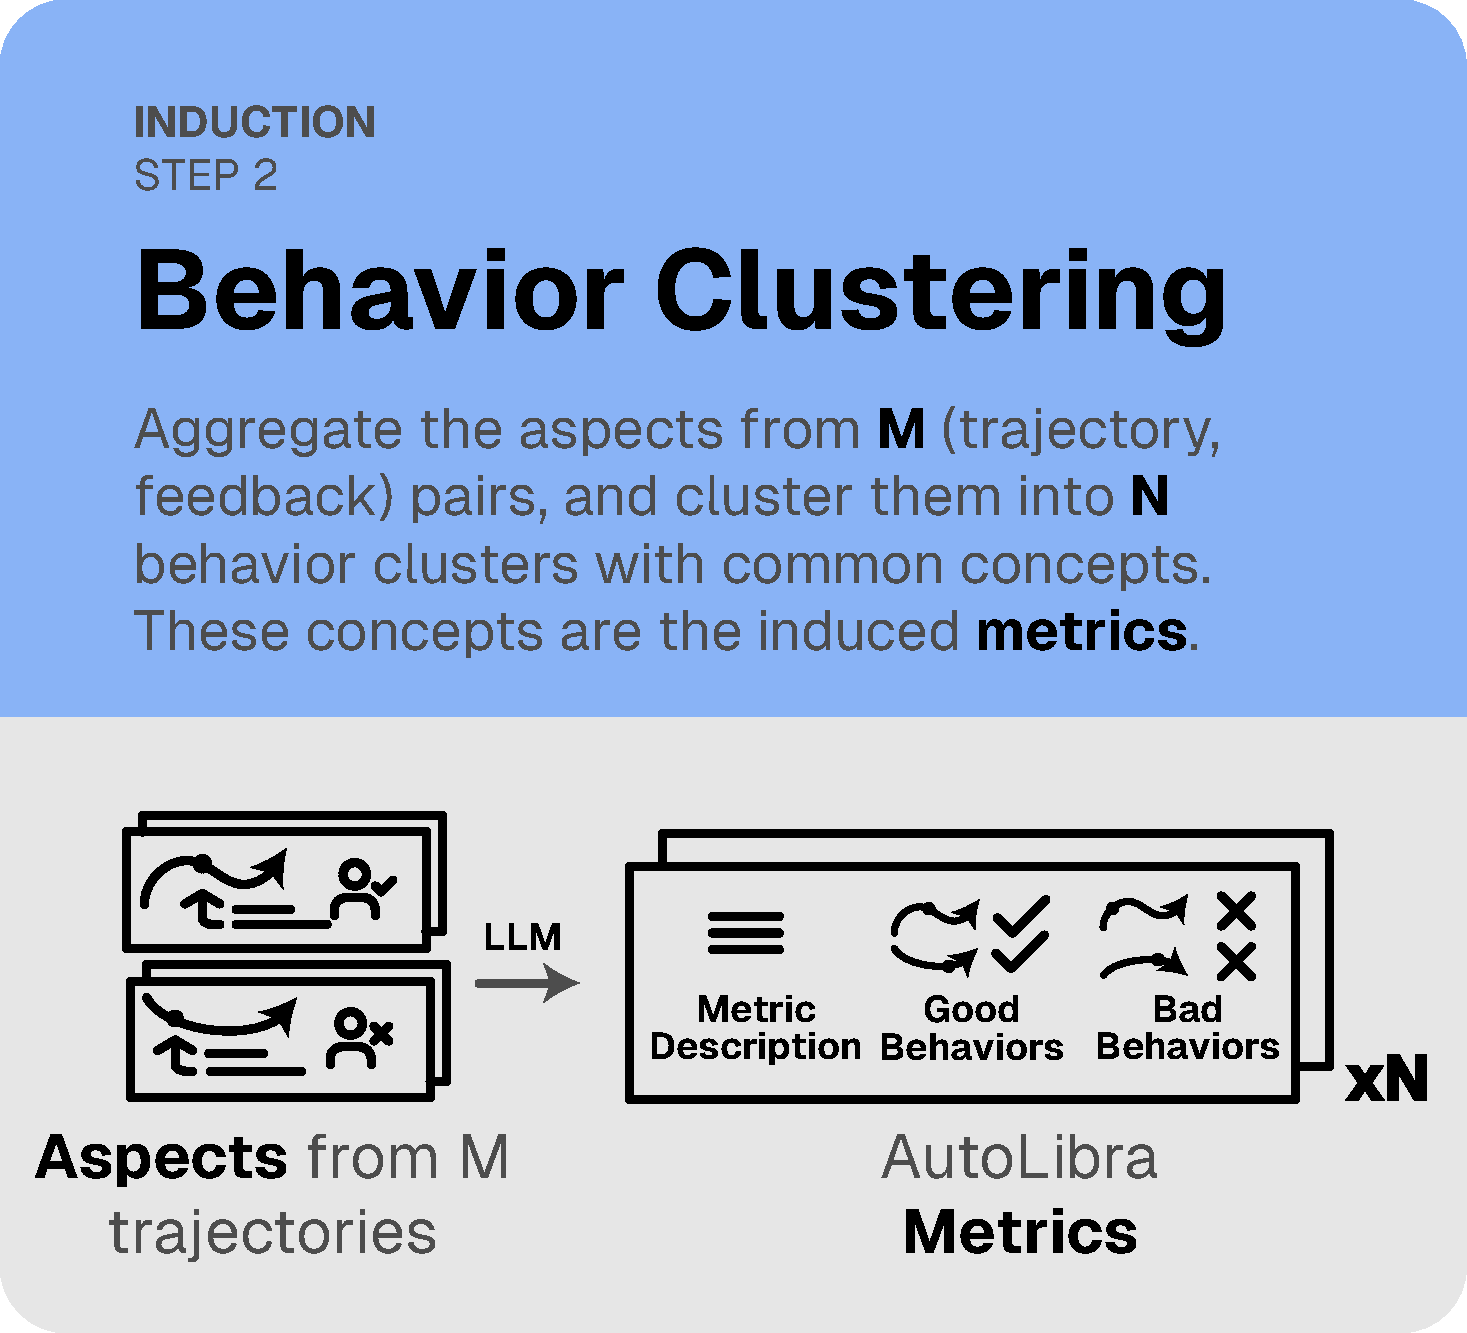
\includegraphics[width=0.4\linewidth]{figs/autolibra_step_2.pdf}
        \caption{Behavior Clustering}
        \label{fig:behavior_clustering}
    \end{figure}

    \begin{figure}[!h]
        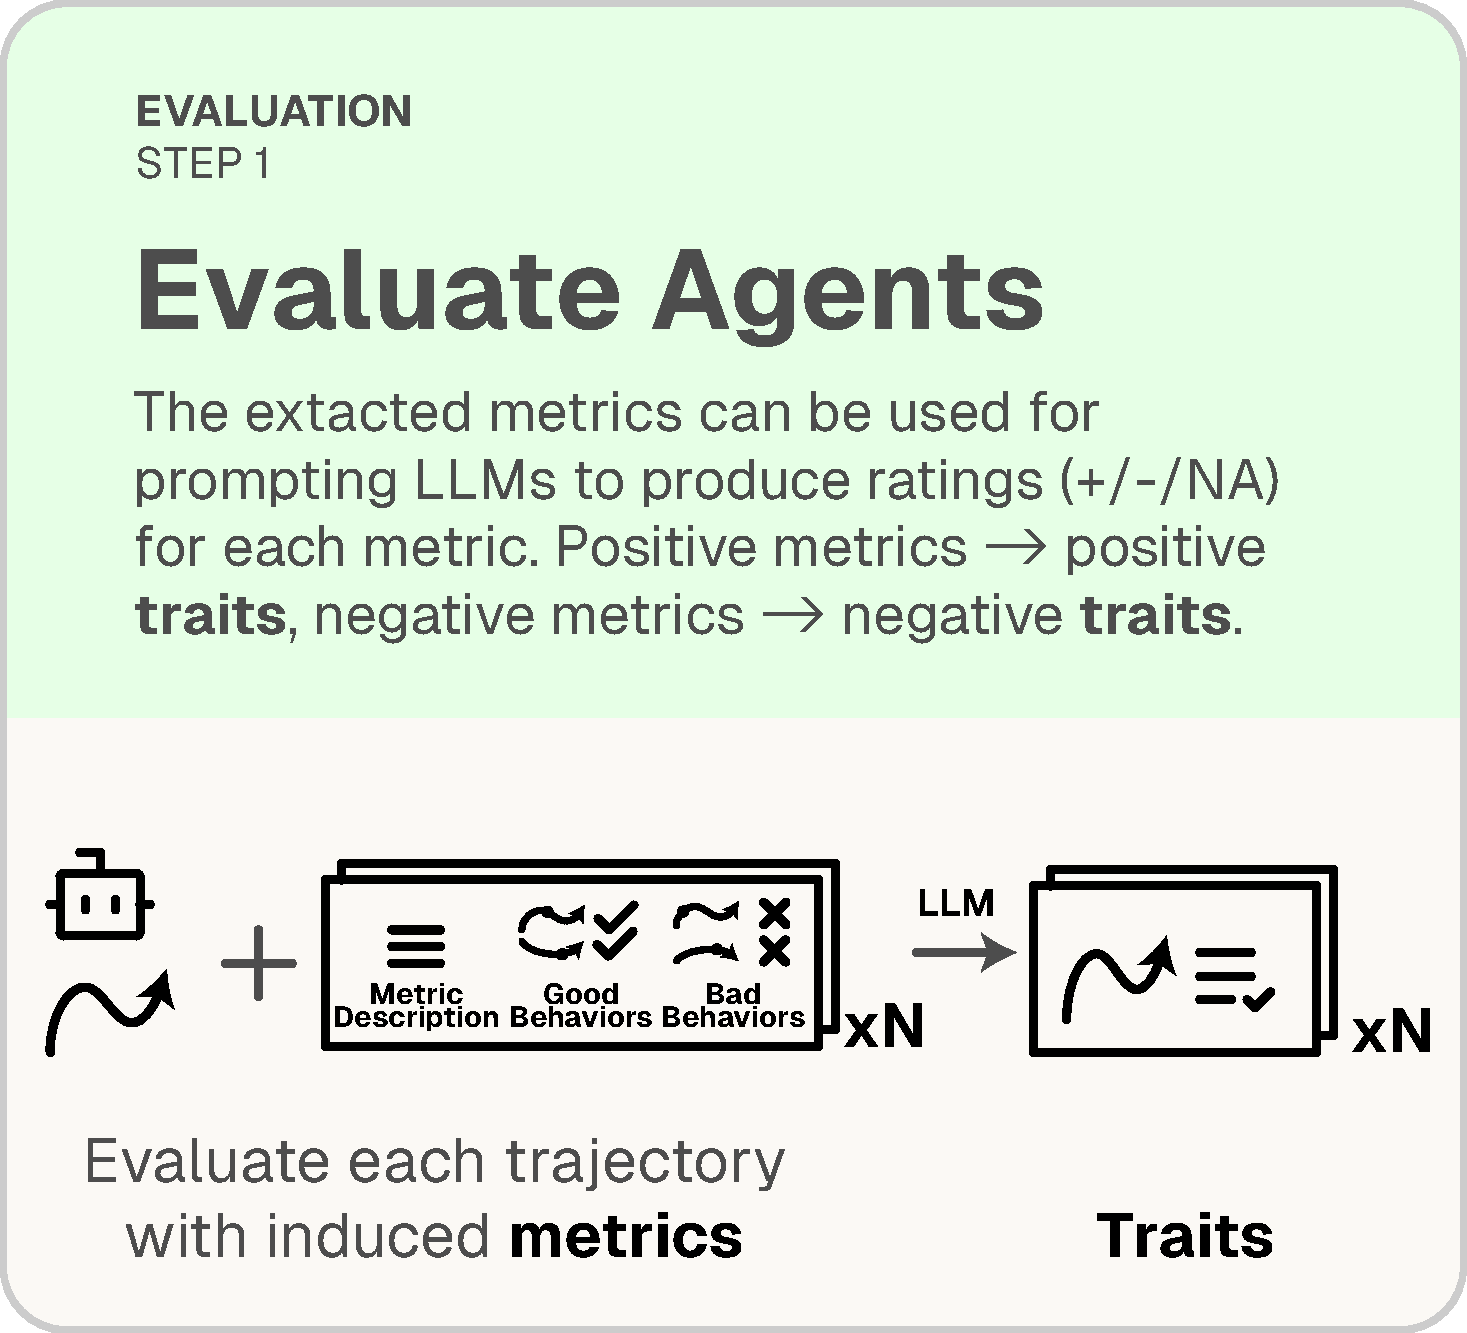
\includegraphics[width=0.4\linewidth]{figs/autolibra_step_3.pdf}
        \caption{Evaluation with induced metrics}
        \label{fig:llm_as_a_judge}
    \end{figure}

    \begin{figure}[!h]
        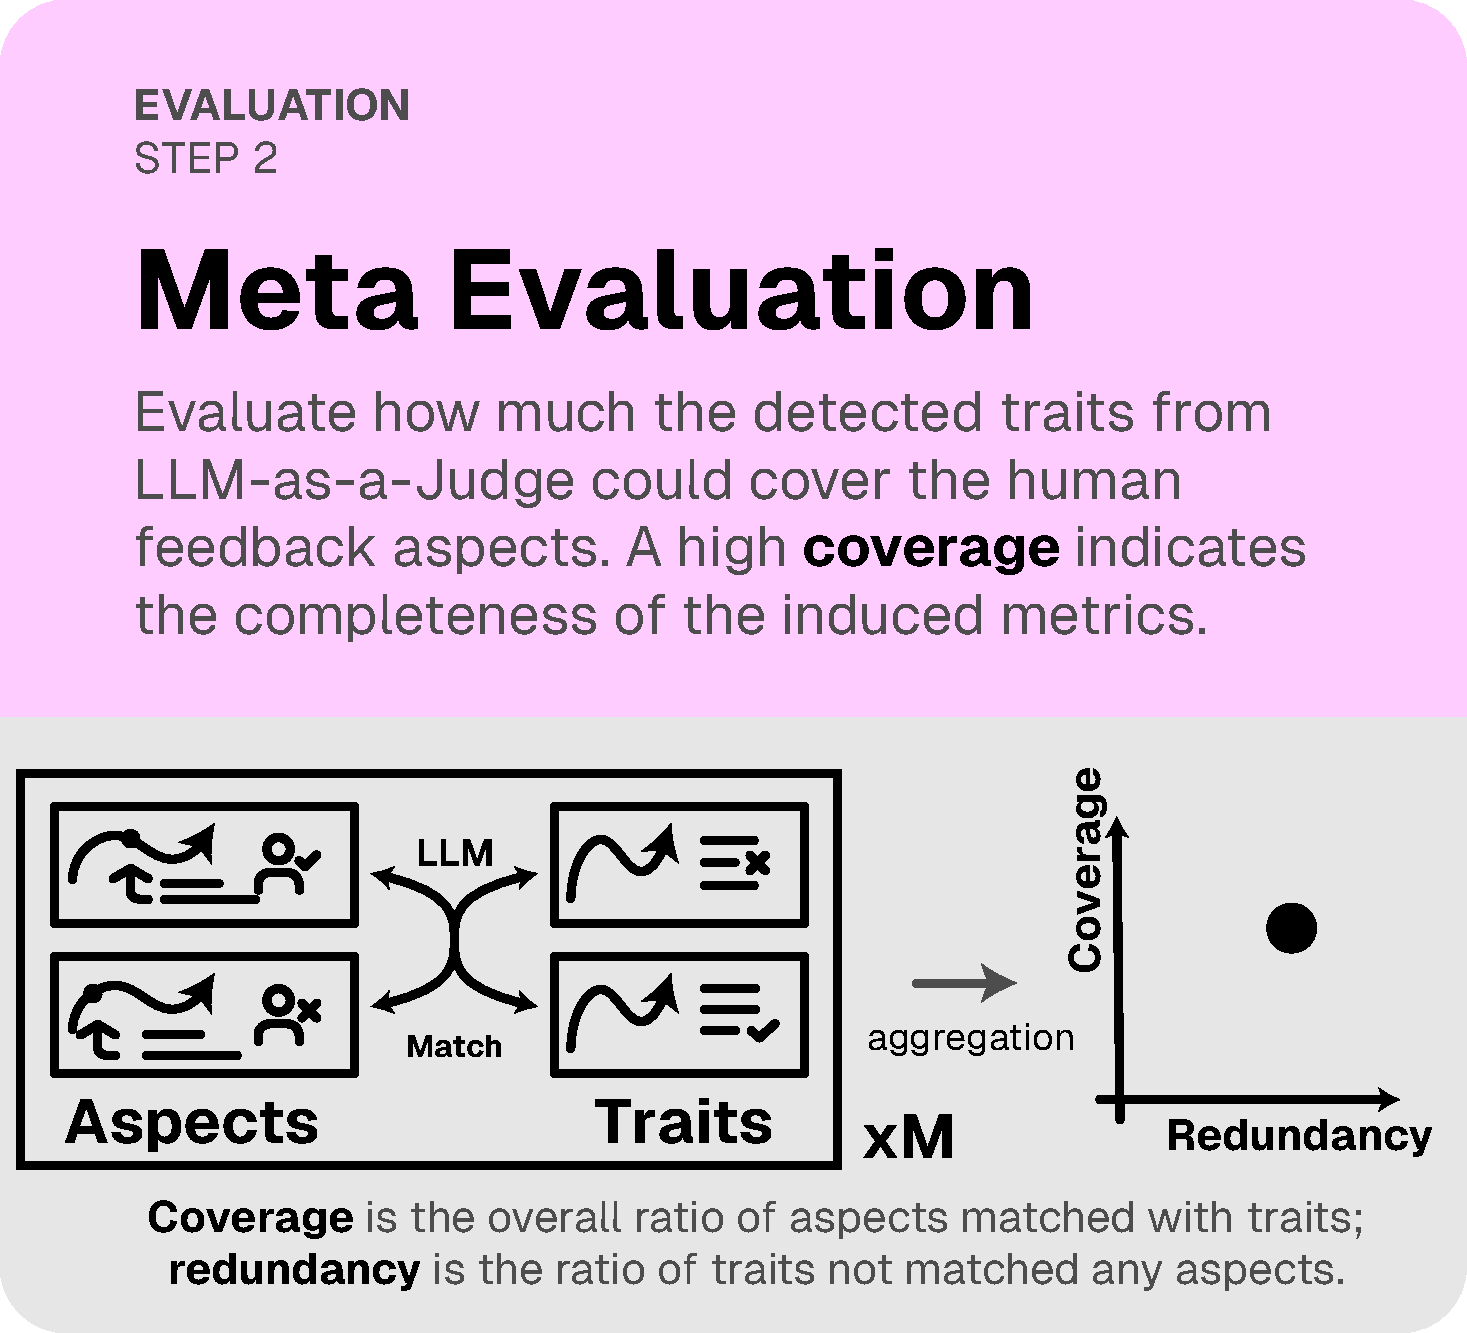
\includegraphics[width=0.4\linewidth]{figs/autolibra_step_4.pdf}
        \caption{Meta evaluation}
        \label{fig:meta_evaluation}
    \end{figure}

    \section{Algorithm of AutoLibra Ladder Experiment}
    \label{appendix:algo1}
    \begin{algorithm}
    \caption{Pseudocode for iterative agent improvement with AutoLibra}
    \begin{algorithmic}[1]
    \For{$i$ in range($n\_iters$)}
        \For{$task$ in $selected\_tasks$}
            \State $traj_i, eval\_score_i += agent.play(task, prompt)$
            \State $annotations_i += editor.annotate(traj_i)$
        \EndFor
        \State $metrics_i = AutoLibra.extract_metrics(traj_i, annotations_i)$
        \State $traj\_scores_i = AutoLibra.llm_eval(metrics_i, traj_i)$
        \State $curr\_scores = eval\_score_i$
        \While {$curr\_scores <= eval\_score_i$}
            \State $prompt = updated\_prompt_k$
            \For{$task$ in $selected\_tasks$}
                \State $\_, curr_scores = agent.play(task, prompt)$
            \EndFor
        \EndWhile
    \EndFor

    \end{algorithmic}
\end{algorithm}



    \section{AutoLibra Ladder Experiment Setup}
    \label{appendix:autolibra_setup}
    This section describes the test configuration used during AutoLibra Ladder
experiments, as described in \ref{sec:ladder}.

For each environment experiment, one unmodified agent is used as a baseline for
comparison (\textit{Iteration 0}), and three complete iterations of iterative
agent improvement with AutoLibra are performed (\textit{Iterations 1-3}), for a
total of four iterations. Six representative tasks for baba-is-ai are used in to
induce metrics within the AutoLibra pipeline, with the remaining 34 tasks held
out for evaluation. The AutoLibra Ladder pipeline is evaluated on the baba-is-ai
and MiniHack environments; any changes to the agent code, the environment score,
trajectory performance, and other metrics are recorded at the end of each iteration.
GPT-4o-241120 \cite{openai2024gpt4ocard} is used as the agent model in all
experiments; the human-in-the-loop configuration of the AutoLibra pipeline is used.

    \section{Baba-is-ai Rules and Environment Configuration}
    \label{appendix:baba_is_ai_rules}
    This section discusses the rules and implementation details of Baba is AI, the task environment used in experiments in Section 4. Baba is AI is derived from Baba is You, a grid-based puzzle video game, and was originally implemented as part of the BALROG \cite{paglieri2024balrog} agent benchmark.

Baba Is You is a puzzle game where the player controls a character that can navigate and modify the rules of the game by pushing blocks containing words such as 'you', 'is' 'key', that, when combined, define the game's rules. 

The game field consists of a rectangular 4-connected grid with a number of objects, rules blocks, and obstacles present.

\begin{figure}[ht]
    \centering
    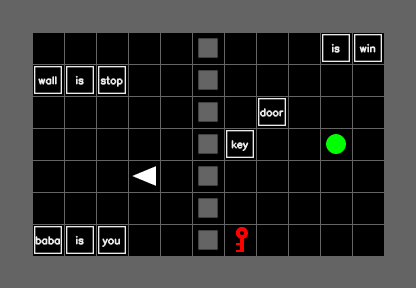
\includegraphics[scale=0.75]{figs/babaisai_env.png}
    \caption{Example of the baba-is-ai environment. In this task (\textit{two\_room-break\_stop-make\_win-distr\_obj-irrelevant\_rule}), the agent has to break the "wall is stop" rule by pushing either 'wall', 'is', or 'stop' out of alignment with the other blocks, and must then push the "key" rule block next to "is win" at (9, 1) to assemble the win rule, then touch the key at (7, 7) to win. Pushing the "door" rule block would be a mistake, as no door object is present.}
    \label{fig:babaisai_env}
\end{figure}

Words (represented as rule blocks) can be combined to form sentences that define the properties of objects, rules, and obstacles in the game, with rules becoming active when a full sequence of rule blocks are joined in a 3-block line horizontally or vertically.

Active rules are built in the form [<subject> <verb> <object>], where the subject and object are the names of objects in the game, and the verb is one of the following: "is", "has", "can", or "not".

The goal of the game is to reach a win condition, by manipulating the rules of the game to create new win conditions, modify the properties of objects, or change the behavior or identity of the player character.

The testing implementation we use is the baba-is-ai environment, a simplified version of Baba is You originally implemented within the BALROG agent benchmark \cite{cloos2024babaaibreakrules, paglieri2024balrog}. This implementation has several simplifications compared to the original game, including a smaller grid size, fewer objects, and a limited set of rules. The environment is designed to be easy to use and understand, while still providing a challenging testbed for evaluating the performance of reinforcement learning agents on agentic reasoning tasks. 

A single baba-is-ai task is defined by an arbitrary rectangular grid where an exit condition must be reached, with several possible obstacles and rules preventing the player from reaching the exit. Intermediate goals to achieving the exit condition can be defined by the user, and the environment will generate a task that requires the agent to learn how to manipulate the rules of the game in order to reach the exit. These intermediate goals are referred to as "subtasks" within our paper, and include:

\begin{itemize}
    \item \textbf{Goto-Win}: The agent must reach a specific location on the grid.
    \item \textbf{Make-Win}: The agent must create a new win condition by manipulating the rules of the game.
    \item \textbf{Break-Stop}: The agent must break or bypass a wall or obstacle in order to reach the exit.
    \item \textbf{Change-You}: The agent must change the identity of the player character in order to reach the exit, by modifying the "baba is you" rule.
\end{itemize}

These subtasks can be arbitrarily combined with distractor objects or rules, immovable game field walls, and each other to generate tasks of varying complexity and length; baba-is-ai implements 40 total unique tasks of gradually increasing difficulty.

The agent is provided observations in a text form, which includes the current state of the game field, the currently active rules, and relative locations of obstacles to the active player character in terms of shortest Manhattan distance. This is done to make the environment compatible with purely text-based language models.

The agent is provided the space of possible actions it can take, which consist moving one space in one of the four cardinal directions (up, down, left, right), but is not given information about whether a given move will result in movement; it is thus free to move into immovable walls without effect, to push rule blocks into corners where they cannot be moved, or to make the task unsolvable by breaking the active "baba is you" rule without taking control of a new object; in this last instance, the environment automatically resets the task to a randomized beginning state for that task.

The environment is limited to 100 steps per task episode to avoid tasks being solved by random walks.

    \section{Baba-is-ai Experiment Results}
    \label{appendix:heldout}
    \renewcommand{\arraystretch}{1.5} 

\begin{table}[ht]  % 'ht' allows LaTeX to place the table here or at the top of the page
\centering
\begin{tabular}{>{\raggedright\arraybackslash}p{6cm}cccc|c}
\toprule
\textbf{Iteration} & \textbf{0} & \textbf{1} & \textbf{2} & \textbf{3} & \textbf{Baseline} \\
\midrule
\textbf{Babaisai Score GPT-4o} & 30\% & 40\% & 43\% & 55\% & 33\% \\
\midrule
\textbf{Babaisai Score Claude 3.5 Sonnet} & 35\% & 40\% & 45\% & 55\% & 37\% \\
\midrule
\textbf{Average Env. Steps} & 79 & 63 & 60 & 51 & - \\
\bottomrule
\end{tabular}
\caption{\raggedright Baba-is-ai Scores and Average Environment Steps}
\label{tab:heldout}
\end{table}


    \section{Baba-is-ai Metric Scores}
    \label{appendix:babaisai}
    % Function to generate color based on percentage value
\newcommand{\cellcolorpercent}[1]{%
\ifdim #1 pt < 10 pt \cellcolor{red!90}%
\else\ifdim #1 pt < 20 pt \cellcolor{red!80}%
\else\ifdim #1 pt < 30 pt \cellcolor{red!70}%
\else\ifdim #1 pt < 40 pt \cellcolor{red!60}%
\else\ifdim #1 pt < 50 pt \cellcolor{red!50}%
\else\ifdim #1 pt < 60 pt \cellcolor{yellow!40}%
\else\ifdim #1 pt < 70 pt \cellcolor{yellow!30}%
\else\ifdim #1 pt < 80 pt \cellcolor{green!30}%
\else\ifdim #1 pt < 90 pt \cellcolor{green!50}%
\else\ifdim #1 pt < 100 pt \cellcolor{green!70}%
\else\cellcolor{green!90}%
\fi\fi\fi\fi\fi\fi\fi\fi\fi\fi }

\makeatletter
\newcommand{\thickhline}{%
\noalign {\ifnum 0=`}\fi \hrule height 3pt \futurelet \reserved@a \@xhline }
\newcolumntype{"}{@{\hskip\tabcolsep\vrule width 1pt\hskip\tabcolsep}} \makeatother

\renewcommand{\arraystretch}{1.5}
\begin{table}[ht]
	\centering
	\begin{tabular}{|>{\arraybackslash}p{5cm}|>{\arraybackslash}p{1.5cm}|c|c|c|c|}
		\hline
		\rowcolor[HTML]{C0C0C0} \textbf{}           & \textbf{Iteration}                                    & \textbf{0}                              & \textbf{1}                              & \textbf{2}                              & \textbf{3}                              \\
		\hline
		Win Condition Recognition                   & 
\includegraphics[scale=0.07]{figs/emojis/emoji_1.png} & \cellcolorpercent{35.0} \textbf{35.0\%} & \cellcolorpercent{55.0} \textbf{55.0\%} & \cellcolorpercent{87.5} \textbf{87.5\%} & \cellcolorpercent{87.5} \textbf{87.5\%} \\
		\hline
		Rule Modification                           & \includegraphics[scale=0.07]{figs/emojis/emoji_2.png} & \cellcolorpercent{0.0} \textbf{0.0\%}   & \cellcolorpercent{10.0} \textbf{10.0\%} & \cellcolorpercent{37.5} \textbf{37.5\%} & \cellcolorpercent{61.9} \textbf{61.9\%} \\
		\hline
		Direct Navigation Efficiency                & \includegraphics[scale=0.07]{figs/emojis/emoji_3.png} & \cellcolorpercent{5.6} \textbf{5.6\%}   & \cellcolorpercent{22.5} \textbf{22.5\%} & \cellcolorpercent{27.5} \textbf{27.5\%} & \cellcolorpercent{37.5} \textbf{37.5\%} \\
		\hline
		Context-Sensitive Decision Making           & \includegraphics[scale=0.07]{figs/emojis/emoji_4.png} & \cellcolorpercent{2.5} \textbf{2.5\%}   & \cellcolorpercent{27.5} \textbf{27.5\%} & \cellcolorpercent{30.0} \textbf{30.0\%} & \cellcolorpercent{37.5} \textbf{37.5\%} \\
		\hline
		Win Rule Construction                       & \includegraphics[scale=0.07]{figs/emojis/emoji_5.png} & \cellcolor[gray]{0.85} 0.0\%            & \cellcolorpercent{0.0} \textbf{0.0\%}   & \cellcolorpercent{0.0} \textbf{0.0\%}   & \cellcolorpercent{5.3} \textbf{5.3\%}   \\
		\hline
		Selective Interaction With Relevant Objects & \includegraphics[scale=0.07]{figs/emojis/emoji_6.png} & \cellcolor[gray]{0.85} 35.0\%           & \cellcolorpercent{40.0} \textbf{40.0\%} & \cellcolorpercent{45.0} \textbf{45.0\%} & \cellcolorpercent{82.5} \textbf{82.5\%} \\
		\hline
		Rule Manipulation and Execution             & \includegraphics[scale=0.07]{figs/emojis/emoji_7.png} & \cellcolor[gray]{0.85} 0.0\%            & \cellcolorpercent{12.5} \textbf{12.5\%} & \cellcolorpercent{31.0} \textbf{31.0\%} & \cellcolorpercent{35.5} \textbf{35.5\%} \\
		\hline
		Subtask Coordination                        & \includegraphics[scale=0.07]{figs/emojis/emoji_8.png} & \cellcolor[gray]{0.85} 2.5\%            & \cellcolor[gray]{0.85} 25.0\%           & \cellcolorpercent{27.5} \textbf{27.5\%} & \cellcolorpercent{35.0} \textbf{35.0\%} \\
		\hline
		Immovable Interaction                       & \includegraphics[scale=0.07]{figs/emojis/emoji_9.png} & \cellcolor[gray]{0.85} 64.9\%           & \cellcolor[gray]{0.85} 69.7\%           & \cellcolor[gray]{0.85} 69.7\%           & \cellcolorpercent{87.9} \textbf{87.9\%} \\
		\thickhline \multicolumn{2}{|c|}{Coverage}  & \textbf{65.0\%}                                       & \textbf{83.0\%}                         & \textbf{85.0\%}                         & \textbf{92.0\%}                          \\
		\hline
		\multicolumn{2}{|c|}{Redundancy}            & \textbf{58.0\%}                                       & \textbf{59.0\%}                         & \textbf{47.0\%}                         & \textbf{59.0\%}                          \\
		\hline
	\end{tabular}
	\caption{Metric Performance for baba-is-ai AutoLibra Iterations 0–3, Across Full
	(40) Environment Tasks}
	\label{tab:metric_perf}
\end{table}
    \newpage

    \section{Baba-is-ai Metric Examples}
    \label{appendix:babaisai_metrics}
    \vspace{-5mm}
\fontsize{9.5pt}{11pt}\selectfont
\begin{tcolorbox}
	[ colback=gray!5!white, colframe=gray!10, title=\textbf{\textcolor{black}{Iteration
	0: Context-Sensitive Decision Making}}]

	\textbf{Explanation:} \\ This metric assesses the agent’s capacity for context-sensitive
	decision making. It evaluates whether the agent tailors its actions according
	to the immediate game conditions—balancing between direct navigation and rule
	modification. Positive behaviors in new environments will demonstrate an ability
	to determine when obstacles require intervention and when direct movement is sufficient,
	thereby optimizing overall efficiency.

	\vspace{1em}
	\textbf{Good Behaviors:}
	\begin{itemize}
		\item Accurately gauges the game context by recognizing when obstacles are not
			an issue—such as when the win condition is already accessible—and refrains
			from unnecessary rule modifications.

		\item Selects focused, goal-oriented actions that align with observed win
			conditions, avoiding extraneous exploration.

		\item Adapts its strategy based on spatial layout and current rules,
			ensuring that its actions are timely and appropriate for the situation.
	\end{itemize}

	\vspace{0.5em}
	\textbf{Bad Behaviors:}
	\begin{itemize}
		\item Engages in excessive exploratory actions that do not contribute to reaching
			the win condition.

		\item Repeatedly takes ineffective actions (for example, persistently moving
			into walls) before finally switching strategy, indicating delayed context-sensitive
			decisions.

		\item Alters irrelevant rules or diverts attention from the active win condition
			when the situation does not demand it.

		\item Fails to adjust decision-making based on contextual cues, leading to
			uncoordinated or delayed progression toward the goal.
	\end{itemize}
\end{tcolorbox}

\fontsize{9.5pt}{11pt}\selectfont
\begin{tcolorbox}
	[ colback=gray!5!white, colframe=gray!30, title=\textbf{\textcolor{black}{Iteration
	1: Rule Modification for Obstacle Management}}]

	\textbf{Explanation:} \\ This metric measures the agent’s competence in managing
	obstacles through rule modifications. It focuses on the agent’s ability to
	detect when a game rule (such as a blocking wall or an unchangeable character assignment)
	is hindering progress and to successfully alter that rule to create a viable
	path to victory. In novel scenarios, agents displaying positive behavior will
	apply targeted rule changes that directly open the path toward the win
	condition.

	\vspace{1em}
	\textbf{Good Behaviors:}
	\begin{itemize}
		\item Proactively breaks the \texttt{'wall is stop'} rule when an obstacle
			blocks access to the win condition.

		\item Effectively modifies rules—such as replacing \texttt{'baba is you'}
			with \texttt{'key'}—to remove or bypass obstacles.
	\end{itemize}

	\vspace{0.5em}
	\textbf{Bad Behaviors:}
	\begin{itemize}
		\item Fails to modify critical rule blocks (for instance, not altering \texttt{'baba
			is you'} when required) that prevent access to the win condition.

		\item Does not interact with immovable obstacles like the \texttt{'wall is stop'}
			rule, neglecting available mechanisms to bypass them.

		\item Neglects to rearrange rule blocks to create or build necessary win conditions
			(e.g., \texttt{'door is win'}), leaving obstacles unaddressed.
	\end{itemize}
\end{tcolorbox}

\fontsize{9.5pt}{11pt}\selectfont
\begin{tcolorbox}
	[ colback=gray!5!white, colframe=gray!60, title=\textbf{\textcolor{black}{Iteration
	2: Subtask Coordination and Overall Task Planning}}]

	\textbf{Explanation:} \\ This metric assesses how well the agent coordinates multiple
	sub-tasks and plans its overall strategy. It rewards behaviors that
	demonstrate clear sequencing – from recognizing obstacles and manipulating
	rules to directly advancing toward the final objective. Failures in subtask coordination
	result in repetitive loops, ineffective transitions between actions, and an inability
	to achieve a meaningful win condition.

	\vspace{1em}
	\textbf{Good Behaviors:}
	\begin{itemize}
		\item Final movement and approach towards \texttt{'ball'} after removing the
			obstacle.

		\item Direct movement between objectives as opposed to unrelated exploration.

		\item Throughout the trajectory, the agent repeatedly chooses actions that
			reduce the distance to the door: moving left and down as needed.

		\item The trajectory demonstrates efficient movement towards the goal without
			unnecessary actions.

		\item The trajectory shows direct movement to the door without redundant backtracking
			or circular movement.

		\item Throughout the trajectory, the agent follows a direct and purposeful
			path towards its goal.
	\end{itemize}

	\vspace{0.5em}
	\textbf{Bad Behaviors:}
	\begin{itemize}
		\item The trajectory shows multiple iterations of upwards movement resulting
			in no significant progress.

		\item In the trajectory, actions such as repeated \texttt{'left'} moves where
			no significant progress towards the goal is made.

		\item In over multiple steps, the agent moves unsuccessfully against
			immovable boundaries and objects.

		\item There are periods in the trajectory where the agent exhibits loops or repetitive
			movements without advancing its position strategically.

		\item Ultimately, the agent's efforts to form victory conditions do not
			result in a meaningful or achievable goal given the map's configuration.
	\end{itemize}
\end{tcolorbox}

\fontsize{9.5pt}{11pt}\selectfont
\begin{tcolorbox}
	[ colback=gray!5!white, colframe=gray!90, title=\textbf{\textcolor{black}{Iteration
	3: Interaction with Immovable Obstacles}}]

	\textbf{Explanation:} \\ This metric measures how the agent handles immovable obstacles.
	Positive behaviors show proper recognition and effective avoidance of fixed
	objects, whereas negative behaviors involve futile or incorrect push attempts that
	betray a lack of understanding of the environment’s static features.

	\vspace{1em}
	\textbf{Good Behaviors:}
	\begin{itemize}
		\item Recognizes that immovable walls or blocks should not be pushed and instead
			plans to bypass them.

		\item Avoids colliding with immovable objects by correctly assessing their fixed
			nature.

		\item Plans actions that account for static obstacles, ensuring safe
			navigation around them.
	\end{itemize}

	\vspace{0.5em}
	\textbf{Bad Behaviors:}
	\begin{itemize}
		\item Repeatedly tries to push into an immovable wall or rule block despite the
			known constraints.

		\item Interacts with stationary obstacles in ways that disregard their immovability,
			leading to ineffective progress.

		\item Executes push commands in the wrong direction on fixed objects,
			indicating a misunderstanding of obstacle dynamics.
	\end{itemize}
\end{tcolorbox}
    \newpage

    \section{Baba-is-ai Prompts}
    \label{appendix:babaisai_prompts}
    \definecolor{lightgreen}{RGB}{220,255,220}
\definecolor{darkgreen}{RGB}{0,150,0}
\newmdenv[ backgroundcolor=lightgreen, linecolor=darkgreen, linewidth=2pt,
roundcorner=5pt, skipabove=10pt, skipbelow=10pt, leftmargin=0pt, rightmargin=0pt,
innerleftmargin=10pt, innerrightmargin=10pt, innertopmargin=10pt,
innerbottommargin=10pt, splittopskip=\topskip, splitbottomskip=10pt, frametitle={\textbf{Iteration 0 Baba-is-ai Prompt}},
frametitlebackgroundcolor=darkgreen, frametitlefont=
\color{white}
\bfseries, frametitlerule=true, frametitleaboveskip=8pt, frametitlebelowskip=8pt,
]{GreenBox}

\begin{GreenBox}
	\textbf{Baba Is You} is a puzzle game where you can manipulate the rules of
	each level. The following are the possible actions you can take in the game,
	followed by a short description of each action:

	\begin{itemize}
		\item \textbf{idle}: wait for one step,

		\item \textbf{up}: take one step up,

		\item \textbf{right}: take one step to the right,

		\item \textbf{down}: take one step down,

		\item \textbf{left}: take one step to the left.
	\end{itemize}

	\textbf{Tips:}
	\begin{itemize}
		\item Examine the level carefully, noting all objects and text blocks
			present.

		\item Identify the current rules, which are formed by text blocks in the
			format "[Subject] IS [Property]" (e.g. "BABA IS YOU").

		\item Consider how you can change or create new rules by moving text blocks around.

		\item Remember that you can only move objects or text that are not defined as
			"STOP" or similar immovable properties.

		\item Your goal is usually to reach an object defined as "WIN", but this can
			be changed.

		\item Think creatively about how changing rules can alter the properties and
			behaviors of objects in unexpected ways.

		\item If stuck, try breaking apart existing rules or forming completely new
			ones.

		\item Sometimes the solution involves making yourself a different object or changing
			what counts as the win condition.
	\end{itemize}

	\textbf{PLAY!}

	\textbf{Current Observation:}

	\textbf{Active rules:}
	\begin{itemize}
		\item ball is win

		\item baba is you
	\end{itemize}

	\textbf{Objects on the map:}
	\begin{itemize}
		\item rule \texttt{ball}: 5 steps to the left and 1 step up

		\item rule \texttt{is}: 4 steps to the left and 1 step up

		\item rule \texttt{win}: 3 steps to the left and 1 step up

		\item ball: 5 steps to the left and 2 steps down

		\item rule \texttt{baba}: 5 steps to the left and 4 steps down

		\item rule \texttt{is}: 4 steps to the left and 4 steps down

		\item rule \texttt{you}: 3 steps to the left and 4 steps down
	\end{itemize}

	First, think about the best course of action. Then, you must choose exactly
	one of the listed actions and output it strictly in the following format:

	\texttt{<|ACTION|>YOUR\_CHOSEN\_ACTION<|END|>}

	Replace \texttt{YOUR\_CHOSEN\_ACTION} with the chosen action.
\end{GreenBox}

\begin{GreenBox}
	[frametitle={\textbf{Iteration 1 Baba-is-ai Prompt}}] \label{box:baba_is_you_iter_1}
	\textbf{Baba Is You} is a puzzle game where you can manipulate the rules of
	each level. The following are the possible actions you can take in the game,
	followed by a short description of each action:

	\begin{itemize}
		\item \textbf{idle}: wait for one step,

		\item \textbf{up}: take one step up,

		\item \textbf{right}: take one step to the right,

		\item \textbf{down}: take one step down,

		\item \textbf{left}: take one step to the left.
	\end{itemize}

	\textbf{Additional Tips:}
	\begin{enumerate}
		\item The game is won by identifying a win condition and making it true by placing
			the "object is win" rule blocks next to each other in line.

		\item First, identify the win condition and where the object corresponding
			to the win condition is located.

		\item If it is blocked, identify the rules that are blocking it and try to
			remove them, or circumvent them by changing the character you control by changing
			the "baba is you" rule.

		\item If the path to the win condition is not blocked, travel directly to
			the win condition object without distractions.

		\item If a "wall is stop" rule is bounded on two sides by walls, the blocks
			cannot be moved, and you must find another way to reach the win condition.

		\item Ignore any objects not related to the win condition, as they are not
			necessary to complete the level.
	\end{enumerate}

	\textbf{Example:}

	\textit{If your observation is:}
	\begin{quote}
		Active rules: ball is win wall is stop baba is you

		Objects on the map: wall 5 steps to the right and 2 steps up \\ rule \texttt{ball}
		8 steps to the right and 2 steps up \\ rule \texttt{is} 9 steps to the right
		and 2 steps up \\ rule \texttt{win} 10 steps to the right and 2 steps up \\ rule
		\texttt{wall} 1 step up \\ rule \texttt{is} 1 step to the right and 1 step up
		\\ rule \texttt{stop} 2 steps to the right and 1 step up \\ wall 5 steps to
		the right and 1 step up \\ rule \texttt{door} 10 steps to the right and 1 step
		up \\ wall 5 steps to the right \\ ball 6 steps to the right \\ wall 5 steps
		to the right and 1 step down \\ wall 5 steps to the right and 2 steps down \\
		wall 5 steps to the right and 3 steps down \\ rule \texttt{baba} 4 steps
		down \\ rule \texttt{is} 1 step to the right and 4 steps down \\ rule \texttt{you}
		2 steps to the right and 4 steps down \\ wall 5 steps to the right and 4
		steps down \\ door 7 steps to the right and 4 steps down \\
	\end{quote}

	\textit{You should reason that:}
	\begin{itemize}
		\item The win condition is "ball is win," therefore you should reach the
			ball to win.

		\item The ball is blocked by a wall, so you should remove the "wall is stop"
			rule.

		\item The "wall is stop" rule is not bounded by walls, so you can move the
			blocks to remove the rule.

		\item The door is not necessary to reach the win condition, so you can
			ignore it.

		\item Once the "wall is stop" rule is removed, you can move directly to the
			ball to win.
	\end{itemize}

	\textbf{PLAY!}

	\textbf{Current Observation:}

	\textbf{Active rules:} baba is you

	\textbf{Objects on the map:}
	\begin{itemize}
		\item rule \texttt{is}: 2 steps to the left and 3 steps up

		\item rule \texttt{win}: 1 step to the left and 3 steps up

		\item key: 2 steps to the right and 2 steps up

		\item rule \texttt{key}: 1 step to the right and 1 step up

		\item rule \texttt{baba}: 3 steps to the left and 2 steps down

		\item rule \texttt{is}: 2 steps to the left and 2 steps down

		\item rule \texttt{you}: 1 step to the left and 2 steps down

		\item ball: 2 steps down

		\item rule \texttt{ball}: 2 steps to the right and 2 steps down
	\end{itemize}

	First, think about the best course of action. Then, you must choose exactly
	one of the listed actions and output it strictly in the following format:

	\texttt{<|ACTION|>YOUR\_CHOSEN\_ACTION<|END|>}
\end{GreenBox}
\newpage
\begin{GreenBox}
	[frametitle={\textbf{Iteration 2 Baba-is-ai Prompt}}]

	\textbf{Baba Is You} is a puzzle game where you can manipulate the rules of each
	level. The following are the possible actions you can take in the game, followed
	by a short description of each action:

	\begin{itemize}
		\item \textbf{idle}: wait for one step,

		\item \textbf{up}: take one step up,

		\item \textbf{right}: take one step to the right,

		\item \textbf{down}: take one step down,

		\item \textbf{left}: take one step to the left.
	\end{itemize}

	\textbf{You solve the puzzle by identifying the type of sub-problem, and then applying
	the following blocks of solution steps:}
	\begin{enumerate}
		\item If the win condition is not blocked and its rule is active, move to
			the win condition object.

		\item If the win condition is blocked by a wall and "wall is stop" rule is active
			and not bounded by the map boundary:
			\begin{enumerate}
				\item Move into the "wall is stop" blocks to remove the rule.

				\item Move to the win condition object.
			\end{enumerate}

		\item If the win condition is blocked by a wall and "wall is stop" rule is active
			and bounded by the map boundary:
			\begin{enumerate}
				\item Locate and move to an object rule block on your side of the wall.

				\item Push the object rule block towards the "baba is you" rule block by
					moving into it, and use this rule block to push the "baba" block out
					of the "baba is you" rule block.
			\end{enumerate}

		\item If the win condition is not active:
			\begin{enumerate}
				\item Locate the object rule block that can be pushed to the "is" rule block
					to activate the win condition.

				\item Push the object rule block to the "is" rule block, making sure
					they are adjacent.

				\item Move to the win condition object.
			\end{enumerate}

		\item If the win condition object is not present:
			\begin{enumerate}
				\item Locate an object rule block that can be pushed to the "is" rule block
					to create the win condition object.

				\item Push the object rule block to the "is" rule block, making sure
					they are adjacent.

				\item Move to the win condition object.
			\end{enumerate}
	\end{enumerate}

	\textbf{Example:}

	\textit{If your observation is:}
	\begin{quote}
		Active rules: wall is stop baba is you

		Objects on the map: wall 3 steps to the right and 3 step up \\ rule \texttt{is}
		7 steps to the right and 3 step up \\ rule \texttt{win} 8 steps to the right
		and 3 step up \\ rule \texttt{wall} 2 step to the left and 2 step up \\ rule
		\texttt{is} 1 step to the left and 2 step up \\ rule \texttt{stop} 2 step up
		\\ wall 3 steps to the right and 2 step up \\ wall 3 steps to the right and 1
		step up \\ key 4 steps to the right and 1 step up \\ wall 3 steps to the right
		\\ rule \texttt{ball} 7 steps to the right \\ wall 3 steps to the right and
		1 step down \\ wall 3 steps to the right and 2 steps down \\ rule \texttt{baba}
		2 step to the left and 3 steps down \\ rule \texttt{is} 1 step to the left
		and 3 steps down \\ rule \texttt{you} 3 steps down \\ wall 3 steps to the right
		and 3 steps down \\ ball 4 steps to the right and 3 steps down\\
	\end{quote}

	\textit{You should plan your actions as follows:}
	\begin{enumerate}
		\item The win condition is not active, so it needs to be built.

		\item The win rule can be built by pushing the "ball" block on the other side
			of the wall next to the "is" block.

		\item The "wall is stop" rule is blocking the path to the ball, so you
			should remove this rule first.

		\item The "wall is stop" rule is not bounded by walls, so you can move the
			blocks to remove the rule.
			\begin{itemize}
				\item Move 2 steps to the left and 2 steps up to reach the "wall is stop"
					rule, and push the "wall" block to remove the rule.
			\end{itemize}

		\item Once the "wall is stop" rule is removed, you can push the "ball" block
			to the "is" block to win.
			\begin{itemize}
				\item Move 7 steps to the right, 3 steps down to reach the "ball" block.

				\item Move 3 steps up to push the "ball" block to the "is" block.
			\end{itemize}

		\item Once you detect the "ball is win" rule as being active, you can move
			directly to the ball to win.
	\end{enumerate}

	\textbf{PLAY!}

	\textbf{Current Observation:}

	\textbf{Active rules:} ball is win baba is you

	\textbf{Objects on the map:}
	\begin{itemize}
		\item rule \texttt{ball}: 3 steps to the left and 3 steps up

		\item rule \texttt{is}: 2 steps to the left and 3 steps up

		\item rule \texttt{win}: 1 step to the left and 3 steps up

		\item ball: 3 steps to the left and 2 steps up

		\item key: 3 steps to the left and 1 step up

		\item rule \texttt{baba}: 3 steps to the left and 2 steps down

		\item rule \texttt{is}: 2 steps to the left and 2 steps down

		\item rule \texttt{you}: 1 step to the left and 2 steps down
	\end{itemize}

	First, think about the best course of action. Then, you must choose exactly one
	of the listed actions and output it strictly in the following format:

	\texttt{<|ACTION|>YOUR\_CHOSEN\_ACTION<|END|>}

	Replace \texttt{YOUR\_CHOSEN\_ACTION} with the chosen action.
\end{GreenBox}
\newpage

\begin{GreenBox}
	[frametitle={\textbf{Iteration 3 Baba-is-ai Prompt}}]

	\textbf{Baba Is You} is a puzzle game where you can manipulate the rules of each
	level. The following are the possible actions you can take in the game, followed
	by a short description of each action:

	\begin{itemize}
		\item \textbf{idle}: wait for one step,

		\item \textbf{up}: take one step up,

		\item \textbf{right}: take one step to the right,

		\item \textbf{down}: take one step down,

		\item \textbf{left}: take one step to the left.
	\end{itemize}

	\textbf{You solve the puzzle by identifying the type of sub-problem, and then applying
	the following blocks of solution steps:}
	\begin{enumerate}
		\item If the win condition is not blocked and its rule is active, move to
			the win condition object.

		\item If the win condition is blocked by a wall and "wall is stop" rule is active
			and not bounded by the map boundary:
			\begin{enumerate}
				\item Move into the "wall is stop" blocks to remove the rule.

				\item Move to the win condition object.
			\end{enumerate}

		\item If the win condition is blocked by a wall and "wall is stop" rule is active
			and bounded by the map boundary:
			\begin{enumerate}
				\item Locate and move to an object rule block on your side of the wall.

				\item Push the object rule block towards the "baba is you" rule block by
					moving into it, and use this rule block to push the "baba" block out
					of the "baba is you" rule block.
			\end{enumerate}

		\item If the win condition is not active:
			\begin{enumerate}
				\item Locate the object rule block that can be pushed to the "is" rule block
					to activate the win condition.

				\item Push the object rule block to the "is" rule block, making sure
					they are adjacent.

				\item Move to the win condition object.
			\end{enumerate}

		\item If the win condition object is not present:
			\begin{enumerate}
				\item Locate an object rule block that can be pushed to the "is" rule block
					to create the win condition object.

				\item Push the object rule block to the "is" rule block, making sure
					they are adjacent.

				\item Move to the win condition object.
			\end{enumerate}
	\end{enumerate}

	\textbf{Example:}

	\textit{If your observation is:}
	\begin{quote}
		\textbf{Active rules:} \\ wall is stop \\ baba is you \\

		\textbf{Objects on the map:} \\ rule \texttt{wall} at (1, 1) \\ rule \texttt{is}
		at (2, 1) \\ rule \texttt{stop} at (3, 1) \\ rule \texttt{is} at (7, 3) \\
		rule \texttt{win} at (8, 3) \\ rule \texttt{ball} at (7, 0) \\ rule \texttt{baba}
		at (5, 6) \\ rule \texttt{is} at (6, 6) \\ rule \texttt{you} at (7, 6) \\
		wall at (4, 0), (4, 1), (4, 2), (4, 3), (4, 4), (4, 5), (4, 6) \\ key at (5,
		1) \\ ball at (5, 6) \\

		\textbf{Current position:} (4, 3) in a grid of shape (1, 0) to (8, 6)
	\end{quote}

	\textit{You should plan your actions as follows:}
	\begin{enumerate}
		\item The win condition is not active, so it needs to be built.

		\item The win rule can be built by pushing the \texttt{ball} block on the
			other side of the wall next to the \texttt{is} block.

		\item The "wall is stop" rule is blocking the path to the ball, so you
			should remove this rule first.

		\item The "wall is stop" rule is not bounded by walls, so you can move the
			blocks to remove the rule.
			\begin{itemize}
				\item Move 2 steps to the left and 2 steps up to reach the "wall is stop"
					rule, and push the \texttt{wall} block to remove the rule.
			\end{itemize}

		\item Once the rule is removed, you can push the \texttt{ball} block to the \texttt{is}
			block.
			\begin{itemize}
				\item Move 7 steps to the right and 3 steps down to reach the \texttt{ball}
					block.

				\item Move 3 steps up to push the \texttt{ball} block to the \texttt{is}
					block.
			\end{itemize}

		\item Once you detect the \texttt{ball is win} rule is active, move directly
			to the ball to win.
	\end{enumerate}

	\textbf{PLAY!}

	\textbf{Current Observation:}

	\textbf{Active rules:} \\ baba is you \\

	\textbf{Objects on the map:}
	\begin{itemize}
		\item rule \texttt{is}: at (2, 1)

		\item rule \texttt{win}: at (3, 1)

		\item key: at (6, 2)

		\item rule \texttt{key}: at (3, 4)

		\item door: at (6, 5)

		\item rule \texttt{baba}: at (1, 6)

		\item rule \texttt{is}: at (2, 6)

		\item rule \texttt{you}: at (3, 6)

		\item rule \texttt{door}: at (6, 6)
	\end{itemize}

	\textbf{Current position:} (4, 3) in a grid of shape (1, 1) to (6, 6)

	\textbf{Rule block pushing physics explanation:}

	\begin{itemize}
		\item Avoid moving into any non-wall rule block unless you are ready to interact
			with it.

		\item Do not push "wall is stop" blocks if the "wall is stop" rule is not currently
			active.
	\end{itemize}

	\textbf{Steps to avoid unwanted interaction:}
	\begin{enumerate}
		\item Read all rule block positions.

		\item Read your current position and direction.

		\item If a rule block is in your path, change direction by 90° (e.g., if going
			up, go left or right).

		\item If a rule is on the wall of the grid, it can only be pushed parallel
			to that wall.
	\end{enumerate}

	\textbf{Example:}

	If you are at (3, 3) and a rule block is at (3, 4), you cannot push it up by first
	moving down. Instead, move to (2, 3) or (4, 3), then move down to (3, 6) to push
	it upward.

	\textbf{Strategic Planning:}

	First, think about your current goal based on the game state. If an active rule
	changes, your goal likely changes too.

	\textbf{Most Important Rule:} If "wall is stop" is active, find a way to
	remove it or gain control of a different object before doing anything else.

	\textbf{Pushing Strategy:}
	\begin{itemize}
		\item Always push blocks upward first (maximum 10 spaces), then push them
			left or right.

		\item Rule \texttt{blocks} are written in backticks. Objects are not. Only
			\texttt{blocks} can be pushed.

		\item Never interact directly with the \texttt{is} or \texttt{win} blocks.
	\end{itemize}

	\textbf{Rule Construction Example:}

	If \texttt{win} is at (11, 1) and \texttt{is} is at (10, 1), place the object rule
	at (9, 1) to form a valid rule.

	\textbf{Coordinate System:}
	\begin{itemize}
		\item Top-left is (1, 1), bottom-right is (x, y).

		\item Moving right increases x, moving down increases y.
	\end{itemize}

	\textbf{Goal Planning Example:}

	\textbf{Active rules:}
	\begin{itemize}
		\item wall is stop — Must be broken under all circumstances!
	\end{itemize}

	\textbf{Steps to achieve the goal:}
	\begin{enumerate}
		\item Break "wall is stop" by moving into its blocks from below.

		\item Build "ball is win" rule.

		\item \texttt{ball} block is at (7, 4), \texttt{is} is at (8, 1). So:
			\begin{itemize}
				\item \texttt{ball} needs to move 3 steps up, 1 step right.

				\item Push from the left (1 step) and from below (3 steps).
			\end{itemize}

		\item If you're at (6, 4), move 1 step down and 1 step right to reach (7, 5),
			then push from below.

		\item Move 3 steps up.
	\end{enumerate}

	Then, you must choose exactly one of the listed actions and output it strictly
	in the following format:

	\texttt{<|ACTION|>YOUR\_CHOSEN\_ACTION<|END|>}
\end{GreenBox}
    \newpage

    \section{Qualitative Observations of baba-is-ai Agent Performance}
    \label{appendix:baba_is_ai_obs}
    The metrics induced by AutoLibra (Table \ref{tab:metrics}) capture the behavior of the agent effectively, with coverage increasing from 65\% at Iteration 0 to 92\% at \emph{Iteration 3} and a low mean redundancy of 56\%. Notably, earlier metrics were found to describe higher-level behaviors than later metrics, reflective of the more complex behaviors that the agent demonstrated in later iterations, as well as the compositionality of induced metrics. Code changes were selected to specifically target given metrics, and as seen in Figure \ref{fig:autolibra-training}, the agent's performance on the targeted metric improved significantly in the iteration following the code change. This demonstrates the utility of AutoLibra for fine-grained agent improvement, as well as the human interpretability of the induced metrics.

The section below discusses iteration-by-iteration induced metrics, code changes directed by the metrics, and the results of these code changes on agent environment and trajectory performance.

\textbf{Iteration 0}
The agent behavior is stochastic and inconsistent, with no clear strategy or goal. Any progress in the environment is the consequence of a random walk. 
\texttt{Win Condition Recognition} \includegraphics[scale=0.07]{figs/emojis/emoji_1.png} was identified as a prerequisite to all other metrics induced in this iteration, as progress in the environment is impossible without recognizing the win condition, and was therefore targeted for improvement. Improvements took the form of few-shot prompting, by supplying an example of observations and the corresponding win condition and subtasks, and guidance on subtask-level planning, by mapping specific environmental observations to actions that would progress the agent towards the win condition.
\textbf{Iteration 1}
An increase in \includegraphics[scale=0.07]{figs/emojis/emoji_1.png} performance of 22\% was observed between \emph{Iteration 0} and \emph{Iteration 1}, indicating that the code changes were effective in improving the agent's ability to recognize the win condition. A slight but statistically insignificant increase was observed for the other metrics induced in \emph{Iteration 0}, but the agent's overall baba-is-ai environment score increased by 10\%, indicating that \includegraphics[scale=0.07]{figs/emojis/emoji_1.png} was correctly identified by AutoLibra as a key bottleneck to the agent's performance in the environment.

The agent now targets specific blocks and objects instead of moving randomly, but gets stuck in loops and on immovable objects, and is unable to consistently complete multi-step tasks.

Based on the metrics induced in \emph{Iteration 1}, several changes to the agent code were implemented:
\begin{itemize}
    \item Augmentation of existing subtask-level planning guidance with low-level position instructions, targeting improvement of \texttt{Rule Modification for Obstacle Management} \includegraphics[scale=0.07]{figs/emojis/emoji_2.png} and \texttt{Direct Navigation Efficiency} \includegraphics[scale=0.07]{figs/emojis/emoji_3.png}
    \item Meta-prompting \cite{Suzgun_Kalai_2024} by providing subtask identification heuristic, targeting improvement of \texttt{Selective Interaction with Relevant Objects} \includegraphics[scale=0.07]{figs/emojis/emoji_6.png} and \texttt{Context-Sensitive Decision Making} \includegraphics[scale=0.07]{figs/emojis/emoji_4.png}
    \item Augmentation of single-shot example with movement instructions, targeting improvement of \texttt{Rule Manipulation and Execution} \includegraphics[scale=0.07]{figs/emojis/emoji_7.png}
\end{itemize}


\textbf{Iteration 2}
Substantial improvements in \includegraphics[scale=0.07]{figs/emojis/emoji_1.png} were observed due to more detailed single-shot examples and reasoning templates, and the corresponding increase in other metrics supports idea that \includegraphics[scale=0.07]{figs/emojis/emoji_1.png} is a key bottleneck to the agent's performance. We further observed a significant increase in \includegraphics[scale=0.07]{figs/emojis/emoji_2.png} and \includegraphics[scale=0.07]{figs/emojis/emoji_7.png}, indicating that the changes targeting these metrics were effective in improving the agent's reasoning performance and consequent avoidance of irrelevant objects. \texttt{Subtask Identification} \includegraphics[scale=0.07]{figs/emojis/emoji_5.png} saw no significant improvement, as the agent still misunderstands map directions and confuses rule blocks with objects. 

Qualitatively, the agent now recognizes when wall rules need to be broken and breaks them, but still cannot assemble rules to win, as it gets stuck on immovable blocks and walls and does not understand where rule blocks need to be placed to form a win condition.

Based on the metrics induced in \emph{Iteration 2}, several changes to the agent code were implemented:
\begin{itemize}
    \item Formatting observations as absolute position (as opposed to relative steps from the agent), and listing of immovable/movable blocks to improve \texttt{Direct Navigation Efficiency} \includegraphics[scale=0.07]{figs/emojis/emoji_3.png}
    \item Chain-of-thought reasoning to assemble subtask completion agenda based on iteration-to-iteration observations, targeting improvement of \texttt{Subtask Coordination and Overall Task Planning} \includegraphics[scale=0.07]{figs/emojis/emoji_8.png}
    \item Augmentation of single-shot example to few-shot example with reasoning templates, targeting improvement of \texttt{Rule Manipulation and Execution} \includegraphics[scale=0.07]{figs/emojis/emoji_7.png}
    \item Explicit instructions on navigation to avoid block collisions and assembly of rules, including movement templates, targeting improvement of \texttt{Rule Manipulation and Execution} \includegraphics[scale=0.07]{figs/emojis/emoji_7.png} and \texttt{Win Rule Construction} \includegraphics[scale=0.07]{figs/emojis/emoji_5.png}
\end{itemize}

\textbf{Iteration 3}
We observe a large increase in \includegraphics[scale=0.07]{figs/emojis/emoji_4.png} and \includegraphics[scale=0.07]{figs/emojis/emoji_6.png}, indicating that the changes targeting these metrics were effective in improving the agent's reasoning performance and consequent avoidance of irrelevant objects. \includegraphics[scale=0.07]{figs/emojis/emoji_3.png} saw further improvement, indicating that the use of absolute position and immovable/movable block listing was effective in improving the agent's navigation efficiency. \includegraphics[scale=0.07]{figs/emojis/emoji_7.png} saw a slight increase, indicating that the changes targeting this metric were effective in improving the agent's ability to manipulate rules to achieve the win condition. \includegraphics[scale=0.07]{figs/emojis/emoji_5.png} saw its first improvement, indicating that more complex metrics are effectively targeted when the base performance and simpler metrics are improved.

Qualitatively, nearly every agent always understands when wall rules can be and cannot be broken, as well as when it's not necessary to break the wall rule, covers nearly all tasks that involve going to win. The agent understands how to assemble win rules but still struggles with changing block direction and understanding that blocks get stuck against walls.
    \newpage

    \section{MiniHack Rules and Environment Configuration}
    \label{appendix:minihack_rules}
    \begin{figure}[ht]
    \centering
    \includegraphics[width=\textwidth]{figs/emojis/maps.png}
    \caption{Overview of representative tasks used in MiniHack agent optimization process with AutoLibra. 
    From left to right, up to down: (1) \emph{Boxoban}, (2) \emph{MazeWalk}, (3) \emph{Corridor Fight}, and (4) \emph{Quest}.}
    \label{fig:minihack_maps}
\end{figure}

This section discusses the rules and implementation details of MiniHack, another task environment used in experiments in Section 4. Similarly to Baba is AI, MiniHack is derived from a grid-based puzzle video game (NetHack), and was originally implemented as part of the BALROG \cite{paglieri2024balrog} agent benchmark.

MiniHack is a grid navigation game expressed in text similar to baba-is-ai, consisting of a procedurally generated environment that requires the agent to navigate a space consisting of various agent roles, creatures, items, and tasks to reach a goal \cite{samvelyan2021minihackplanetsandboxopenended}. Given its plasticity and abundant elements, MiniHack is more complex, challenging, and diversified than baba-is-ai; this is reflected in a lower success rate for agents on MiniHack versus Baba is AI, with a baseline agent task completion rate of 10\% on MiniHack vs 33\% on baba-is-ai \cite{paglieri2024balrog}.

Similar to our experiments with baba-is-ai, the Ladder improvement process for MiniHack also follows the algorithm detailed in Appendix \ref{appendix:algo1}. Two full iterations of agent improvement with AutoLibra were performed on MiniHack. Four representative tasks for MiniHack are used in iterative metric improvement, with the remainder held out for evaluation. The agent is evaluated on the MiniHack environment and any changes to the agent code at the beginning of each iteration, and the environment score, trajectory performance, and other metrics are recorded at the end of each iteration. GPT-4o-241120 is used as the agent model.\\

The four selected representative tasks each contain a unique subset of subtasks evaluating an agent's capability. Figure \ref{fig:minihack_maps} shows an example for each task, and from left to right, up to down, these maps respectively represent Boxoban, MazeWalk, Corridor Fight, and Quest. 

\p{\textbf{Boxoban} is a box-pushing puzzle game inspired by Sokoban, rendered within the MiniHack environment. To succeed in Boxoban, the agent needs to push the four boulders (orange balls) onto the four fountains (blue icons), and partial credit will be awarded for pushing some of the boulders onto the fountains. Boxoban tests the agent's capability in strategic planning and rule-following.}
\newline
\\
\p{\textbf{MazeWalk} is a game that requires the agent to explore unknown dark spaces to find the target exit staircase (the icon with a downward arrow). Two challenges for MazeWalk are fog of war -- the agent initially lacks information about areas of the map it hasn't visited, and must explore to discover the map and maze layout, and darkness -- even if the agent has visited a block, the block will become 'dark' as the agent walks away and it passes out of view, retaining information about its layout but not any enemies or items present. Thus, MazeWalk tests the agent's capability in map memory and strategic searching.}
\newline
\\
\p{\textbf{Corridor Fight} is a game that requires the agent to explore an unknown dark corridor map to find the target exit staircase while engaging or avoiding giant rat enemies. Corridor Fight tests the agent's capability in memory, space awareness, hazard awareness, and strategic combat.}
\newline
\\
\p{\textbf{Quest} requires the agent to use a tool to help itself cross an otherwise impassable wall of lava, survive randomly generated monsters, and search for the target exit staircase. As the most subtask-rich and randomized game, it tests the agent's abilities to recognize and utilize tools, understand its role and special power, and strategically survive from monsters.}

In all tasks, the agent is provided observations in a text form, which includes the current state of the game field, the currently active rules, and relative locations of obstacles to the active player character in terms of shortest Manhattan distance. This is done to make the environment compatible with purely text-based language models.

The environment is limited to 100 steps per task episode to avoid tasks being solved by random walks.

    \section{MiniHack Experiment Results}
    \label{appendix:heldout_mini}
    \begin{table}[h]
	\centering
	\renewcommand{\arraystretch}{1.5}
	\begin{tabular}{p{4cm}ccc|c}
		\toprule \textbf{Turn}                  & \textbf{0} & \textbf{1} & \textbf{2} & \textbf{Baseline} \\
		\midrule \textbf{MiniHack Score GPT-4o} & 0\%        & 12.5\%     & 25\%       & 10\%              \\
		\midrule \textbf{Average Env. Steps}    & 85         & 91         & 88         & -                 \\
		\bottomrule
	\end{tabular}
	\caption{MiniHack Score and Average Environment Steps}
	\label{tab:heldout_mini}
\end{table}

    \section{MiniHack Metric Performance}
    \label{appendix:minihack}
    \renewcommand{\arraystretch}{1.5}
\begin{table}[ht]
	\centering
	\begin{tabular}{|>{\arraybackslash}p{6cm}|>{\arraybackslash}p{1.5cm}|c|c|c|}
		\hline
		\rowcolor[HTML]{C0C0C0} \textbf{}                & \textbf{Iteration}                                   & \textbf{0}                                & \textbf{1}                                & \textbf{2}                                \\
		\hline
		% Row 1
		Target Navigation Effectiveness                  & \includegraphics[scale=0.09]{figs/emojis/mini_1.png} & \cellcolorpercent{16.67} \textbf{16.67\%} & \cellcolorpercent{8.33} \textbf{8.33\%}   & \cellcolorpercent{41.67} \textbf{41.67\%} \\
		\hline
		% Row 2
		Efficient Exploration and Map Memory Utilization & \includegraphics[scale=0.07]{figs/emojis/mini_2.png} & \cellcolorpercent{16.67} \textbf{16.67\%} & \cellcolorpercent{0.00} \textbf{0.00\%}   & \cellcolorpercent{25.00} \textbf{25.00\%} \\
		\hline
		% Row 3
		Hazard Awareness and Equipment Utilization       & \includegraphics[scale=0.09]{figs/emojis/mini_3.png} & \cellcolorpercent{0.00} \textbf{0.00\%}   & \cellcolorpercent{0.00} \textbf{0.00\%}   & \cellcolorpercent{0.00} \textbf{0.00\%}   \\
		\hline
		% Row 4
		Boulder Manipulation Strategy                    & \includegraphics[scale=0.09]{figs/emojis/mini_4.png} & \cellcolorpercent{0.00} \textbf{0.00\%}   & \cellcolorpercent{0.00} \textbf{0.00\%}   & \cellcolorpercent{0.00} \textbf{0.00\%}   \\
		\hline
		% Row 5
		Combat Engagement and Survival                   & \includegraphics[scale=0.09]{figs/emojis/mini_5.png} & \cellcolorpercent{8.33} \textbf{8.33\%}   & \cellcolorpercent{8.33} \textbf{8.33\%}   & \cellcolorpercent{25.00} \textbf{25.00\%} \\
		\hline
		% Row 6
		Role-Specific Ability Utilization                & \includegraphics[scale=0.07]{figs/emojis/mini_6.png} & \cellcolorpercent{0.00} \textbf{0.00\%}   & \cellcolorpercent{0.00} \textbf{0.00\%}   & \cellcolorpercent{0.00} \textbf{0.00\%}   \\
		\hline
		% Row 7
		Spatial Awareness and Interpretation             & \includegraphics[scale=0.08]{figs/emojis/mini_7.png} & {-}                                       & \cellcolorpercent{16.67} \textbf{16.67\%} & \cellcolorpercent{58.33} \textbf{58.33\%} \\
		\hline
		% Row 8
		Object Pickup Efficiency                         & \includegraphics[scale=0.08]{figs/emojis/mini_8.png} & {-}                                       & \cellcolorpercent{0.00} \textbf{0.00\%}   & \cellcolorpercent{0.00} \textbf{0.00\%}   \\
		\hline
		% Row 9
		Giant Rats Encounter Handling                    & \includegraphics[scale=0.08]{figs/emojis/mini_9.png} & {-}                                       & {-}                                       & \cellcolorpercent{25.00} \textbf{25.00\%} \\
		\thickhline                                       % Coverage and Redundancy
		\multicolumn{2}{|c|}{Coverage}                   & 82.89\%                                              & 81.82\%                                   & 87.84\%                                    \\
		\hline
		\multicolumn{2}{|c|}{Redundancy}                 & 61.11\%                                              & 65.63\%                                   & 71.30\%                                    \\
		\hline
	\end{tabular}
	\caption{Metric Performance for MiniHack AutoLibra Iterations 0–2}
	\label{tab:metric_mini_perf}
\end{table}
    \newpage

    \section{MiniHack Metric Examples}
    \label{appendix:minihack_metrics}
    \fontsize{9.5pt}{11pt}\selectfont
\begin{tcolorbox}[breakable, colback=gray!10!white, colframe=gray!50!black, title=\textbf{Iteration 0: Target Navigation Effectiveness}]

\textbf{Explanation:} \\
This metric evaluates the agent’s ability to accurately identify and navigate toward key goal locations (e.g., the downward stairs). Positive behaviors show clear planning and directional focus, while negative examples reveal distractions or failures in goal-oriented movement.

\vspace{1em}
\textbf{Good Behaviors:}
\begin{itemize}
  \item Behavior: The agent decides to move south and reaches the downward stairs.
  \item Behavior: The agent’s reasoning shows it plans its action to reach the stairs.
  \item Behavior: From its reasoning, the agent appears to recognize the goal of locating the stairs downward.
  \item Behavior: From the trajectory and reasoning, the agent consistently aimed toward the general direction of its goal—the stairs down.
\end{itemize}

\vspace{0.5em}
\textbf{Bad Behaviors:}
\begin{itemize}
  \item Behavior: The repeated attempts to kick the goblin instead of progressing towards the stairs.
  \item Behavior: The agent repeatedly interacts with adjacent stairs up but does not visibly attempt to identify or locate downward stairs.
  \item Behavior: The agent explored the map but did not identify the downward stair in its trajectory.
  \item Behavior: Throughout the trajectory, the agent did not manage to locate the downward stairs, despite exploring various places in the environment.
  \item Behavior: The agent spends multiple actions traversing the map without making meaningful progress toward the downward stairs.
  \item Behavior: Performed in the sequence of actions where the agent explores but eventually doesn't find the stairway downward, ending the session unsuccessfully.
  \item Behavior: During its navigation, the agent didn't succeed in reaching the stairs down.
\end{itemize}

\end{tcolorbox}

    \newpage

    \section{MiniHack Prompts}
    \label{appendix:minihack_prompts}
    \definecolor{lightgreen}{RGB}{220,255,220}
\definecolor{darkgreen}{RGB}{0,150,0}
\newmdenv[ backgroundcolor=lightgreen, linecolor=darkgreen, linewidth=2pt,
roundcorner=5pt, skipabove=10pt, skipbelow=10pt, leftmargin=0pt, rightmargin=0pt,
innerleftmargin=10pt, innerrightmargin=10pt, innertopmargin=10pt,
innerbottommargin=10pt, splittopskip=\topskip, splitbottomskip=10pt, frametitle={\textbf{Iteration 0 MiniHack Prompt}},
frametitlebackgroundcolor=darkgreen, frametitlefont={\color{white}\bfseries},
frametitlerule=true, frametitleaboveskip=8pt, frametitlebelowskip=8pt, ]{MyGreenBox}
\BeforeBeginEnvironment{MyGreenBox}{\VerbatimEnvironment\small}

%% MiniHack Instruction Prompt Template
% Requires mdframed and defined GreenBox environment as before
\begin{MyGreenBox}
	[frametitle={\textbf{Iteration 0 MiniHack Prompt}}] You are an agent playing MiniHack.
	The following are the possible actions you can take in the game, followed by a
	short description of each action:

	\begin{itemize}
		\item \textbf{north}: move north,

		\item \textbf{east}: move east,

		\item \textbf{south}: move south,

		\item \textbf{west}: move west,

		\item \textbf{northeast}: move northeast,

		\item \textbf{southeast}: move southeast,

		\item \textbf{southwest}: move southwest,

		\item \textbf{northwest}: move northwest,

		\item \textbf{far north}: move far north,

		\item \textbf{far east}: move far east,

		\item \textbf{far south}: move far south,

		\item \textbf{far west}: move far west,

		\item \textbf{far northeast}: move far northeast,

		\item \textbf{far southeast}: move far southeast,

		\item \textbf{far southwest}: move far southwest,

		\item \textbf{far northwest}: move far northwest,

		\item \textbf{up}: go up the stairs,

		\item \textbf{down}: go down the stairs,

		\item \textbf{wait}: rest one move while doing nothing,

		\item \textbf{more}: display more of the message,

		\item \textbf{apply}: apply (use) a tool,

		\item \textbf{close}: close an adjacent door,

		\item \textbf{open}: open an adjacent door,

		\item \textbf{eat}: eat something,

		\item \textbf{force}: force a lock,

		\item \textbf{kick}: kick an enemy or a locked door or chest,

		\item \textbf{loot}: loot a box on the floor,

		\item \textbf{pickup}: pick up things at the current location if there are any,

		\item \textbf{pray}: pray to the gods for help,

		\item \textbf{puton}: put on an accessory,

		\item \textbf{quaff}: quaff (drink) something,

		\item \textbf{search}: search for hidden doors and passages,

		\item \textbf{zap}: zap a wand
	\end{itemize}

	% Conditional Goal Statements
	\textbf{For task which name consists "corridor":}\
Your goal is to explore the level
	and reach the stairs down.

	\textbf{For task which name consists “quest”:}\
Your goal is to explore the
	level, fight monsters, and navigate rooms and mazes to ultimately reach the
	stairs down.

	\textbf{For task which name consists “boxoban”:}\
You are playing Boxoban, a
	box-pushing game inspired by Sokoban. Your goal is to push the boulders onto the
	fountains on the map. You can push the boulders by walking into them, as long as
	there are no obstacles behind them.

	\textbf{For task which name consists “mazewalk”:}\
Your goal is to explore the
	level and reach the stairs down.

	\textbf{Otherwise:}\
Your goal is to get as far as possible in the game.

	In a moment I will present a history of actions and observations from the game.

	\textbf{Tip:} there is no point in outputting the same action over and over if
	nothing changes.

	% Optional Feedback Section
	\textbf{Additional Feedback (if provided):}\
I will also present lists of positive
	and negative feedback based on your previous attempts on this task, use this
	information to change your strategy and improve your performance. \
\texttt{Positive:
	{positive}}\
\texttt{Negative: {negative}}

	\textbf{PLAY!}
\end{MyGreenBox}

%turn_1
\begin{MyGreenBox}
	[frametitle={\textbf{Iteration 1 MiniHack Prompt}}] You are an agent playing MiniHack.
	The following are the possible actions you can take in the game, followed by a
	short description of each action:

	\begin{itemize}
		\item \textbf{north}: move north,

		\item \textbf{east}: move east,

		\item \textbf{south}: move south,

		\item \textbf{west}: move west,

		\item \textbf{northeast}: move northeast,

		\item \textbf{southeast}: move southeast,

		\item \textbf{southwest}: move southwest,

		\item \textbf{northwest}: move northwest,

		\item \textbf{far north}: move far north,

		\item \textbf{far east}: move far east,

		\item \textbf{far south}: move far south,

		\item \textbf{far west}: move far west,

		\item \textbf{far northeast}: move far northeast,

		\item \textbf{far southeast}: move far southeast,

		\item \textbf{far southwest}: move far southwest,

		\item \textbf{far northwest}: move far northwest,

		\item \textbf{up}: go up the stairs,

		\item \textbf{down}: go down the stairs,

		\item \textbf{wait}: rest one move while doing nothing,

		\item \textbf{more}: display more of the message,

		\item \textbf{apply}: apply (use) a tool,

		\item \textbf{close}: close an adjacent door,

		\item \textbf{open}: open an adjacent door,

		\item \textbf{eat}: eat something,

		\item \textbf{force}: force a lock,

		\item \textbf{kick}: kick an enemy or a locked door or chest,

		\item \textbf{loot}: loot a box on the floor,

		\item \textbf{pickup}: pick up things at the current location if there are any,

		\item \textbf{pray}: pray to the gods for help,

		\item \textbf{puton}: put on an accessory,

		\item \textbf{quaff}: quaff (drink) something,

		\item \textbf{search}: search for hidden doors and passages,

		\item \textbf{zap}: zap a wand
	\end{itemize}

	% Corridor-specific
	\textbf{For task name contains “corridor”:}\\ Your goal is to explore the
	level and reach the stairs down.

	\textbf{Notes:}
	\begin{enumerate}
		\item The target stairs down is always at the other room on the map, so you
			should prioritize exploring the other room.

		\item Whenever you encounter a monster (giant rat) in a room, you should
			always try to run to the direction of the corridor.

		\item Whenever you encounter a monster (giant rat) on the corridor, you
			should always try to kill the monster (giant rat).

		\item Once you reach the second room on the map, you should explore the room
			fully to find the target stairs down, but whenever you encounter a monster
			(giant rat), you should always try to run to the direction of the corridor.
	\end{enumerate}

	\textbf{Example:} \begin{verbatim}
                        ---
                        .<|
                        ..@#
                         .|
\end{verbatim}

	% Quest-specific
	\textbf{For task name contains “quest”:}\\ Your goal is to explore the level, fight
	monsters, and navigate rooms and mazes to ultimately reach the stairs down.

	\textbf{Notes:}
	\begin{enumerate}
		\item You should never cross (lava) without necessary ability or equipment.

		\item Always explore the area approachable (no need to cross the lava) well enough
			to find sufficient support. Below is an example:
	\end{enumerate}

	\textbf{Map Example:} \begin{verbatim}
                        --------------
                        |@....}......---
                        |.(...}.......F-
                        |.....}.....................|
                        |.....}........--------     |
                        |.....}......---
                        --------------
\end{verbatim}

	\begin{enumerate}
		\setcounter{enumi}{2}

		\item You should always try to apply the tool you can get, even though you
			do not know the effect.

		\item You should always try to apply your role's ability, even though you do
			not know the effect.
	\end{enumerate}

	% Boxoban-specific
	\textbf{For task name contains “boxoban”:}\\ You are playing Boxoban, a box-pushing
	game inspired by Sokoban. Your goal is to push the boulders onto the fountains
	on the map. You can push the boulders by walking into them, as long as there are
	no obstacles behind them.

	\textbf{Notes:} For this task, you should follow the below rules with priority
	from top to down:
	\begin{enumerate}
		\item You should remember the locations of the fountains in the beginning.

		\item You should never push a boulder in a direction if in this direction,
			the next spot next to the boulder is not empty or is not the fountain.

		\item You should never push a boulder to any L-shaped wall configuration (two
			adjacent walls).
	\end{enumerate}

	\textbf{Example (dead corner):}
	\begin{verbatim}
                                  ##########
                                  #`.....###
\end{verbatim}

	\begin{enumerate}
		\setcounter{enumi}{3}

		\item You should never push a boulder next to a wall unless, in the
			direction perpendicular to the line joining the boulder and its neighbor
			wall, there is at least one fountain left open such that between this fountain
			and the boulder all spots are empty.

		\item You should never push a boulder if it is already on the fountain.

		\item If a boulder and a fountain are on the same row or column, and all
			spots between this boulder and this fountain are empty, and the first spot
			next to the boulder on the opposite direction of which the fountain locates
			is empty, you should always push this boulder to the corresponding
			fountain.
	\end{enumerate}

	\textbf{Map Example (established path):} \begin{verbatim}
                                  ##########
                                  #......<##
                                  #.#@.{`.##
                                  #.``##.#.#
                                  #..`...{.#
                                  #.#.{....#
                                  #######.{#
                                  #######..#
                                  #######..#
                                  ##########
\end{verbatim}

	\textbf{Example (dead corner reminder):} \begin{verbatim}
                                  ##########
                                  #`.....###
\end{verbatim}

	% MazeWalk-specific
	\textbf{For task name contains “mazewalk”:}\\ Your goal is to explore the
	level and reach the stairs down.

	\textbf{Notes:} For this task, your action space will be limited to: \begin{verbatim}
{"north": "move north",
 "east":  "move east",
 "south": "move south",
 "west":  "move west"}
\end{verbatim}

	You will not choose any actions other than these four. Follow strictly:
	\begin{enumerate}
		\item If the block on your east is empty, move east.

		\item If east is blocked and north is open, move north.

		\item If east and north are both blocked, and west is open, move west.

		\item If east, north, and west are blocked, move south.
	\end{enumerate}

	% Default
	\textbf{Otherwise:}\\ Your goal is to get as far as possible in the game.

	In a moment I will present a history of actions and observations from the game.

	\textbf{Tip:} there is no point in outputting the same action over and over if
	anything changes.

	\textbf{PLAY!}
\end{MyGreenBox}

%turn_2
\begin{MyGreenBox}
	[frametitle={\textbf{Iteration 2 MiniHack Prompt}}] You are an agent playing MiniHack.
	The following are the possible actions you can take in the game:

	\begin{itemize}
		\item \textbf{north}: move north,

		\item \textbf{east}: move east,

		\item \textbf{south}: move south,

		\item \textbf{west}: move west,

		\item \textbf{northeast}: move northeast,

		\item \textbf{southeast}: move southeast,

		\item \textbf{southwest}: move southwest,

		\item \textbf{northwest}: move northwest,

		\item \textbf{far north}: move far north,

		\item \textbf{far east}: move far east,

		\item \textbf{far south}: move far south,

		\item \textbf{far west}: move far west,

		\item \textbf{far northeast}: move far northeast,

		\item \textbf{far southeast}: move far southeast,

		\item \textbf{far southwest}: move far southwest,

		\item \textbf{far northwest}: move far northwest,

		\item \textbf{up}: go up the stairs,

		\item \textbf{down}: go down the stairs,

		\item \textbf{wait}: rest one move while doing nothing,

		\item \textbf{more}: display more of the message,

		\item \textbf{apply}: apply (use) a tool,

		\item \textbf{close}: close an adjacent door,

		\item \textbf{open}: open an adjacent door,

		\item \textbf{eat}: eat something,

		\item \textbf{force}: force a lock,

		\item \textbf{kick}: kick an enemy or a locked door or chest,

		\item \textbf{loot}: loot a box on the floor,

		\item \textbf{pickup}: pick up things at the current location if there are any,

		\item \textbf{pray}: pray to the gods for help,

		\item \textbf{puton}: put on an accessory,

		\item \textbf{quaff}: quaff (drink) something,

		\item \textbf{search}: search for hidden doors and passages,

		\item \textbf{zap}: zap a wand
	\end{itemize}

	% Corridor-specific
	\textbf{For task name contains “corridor”:}\\ \textbf{Your goal:} Your goal is
	to explore the level and reach the stairs down.

	\textbf{Notes:}

	Most important notice before you start: "." in the map means room, so if your
	current space is marked by "." you are in the room. In the map, "\#" means
	corridor. You should never misrecognize the type of location you are currently
	at as this is crucial for your game. Always be certain about your current
	location before you decide an action.

	\textit{You should permanently treat “<” the same as “.”}

	\begin{enumerate}
		\item The target stairs down is always at the other room on the map, so you
			should prioritize exploring the other room. Remember, the goal spot is
			always at the far east of the map.

		\item Whenever you haven’t moved onto the corridor (“\#”) yet, find one “\#”
			as soon as possible and move onto it.
	\end{enumerate}

	\textbf{Example:}
	\begin{verbatim}
                        ---
                        .<|
                        ..@#
                         .|
\end{verbatim}

	\textbf{Example:}
	\begin{verbatim}
                      -----
                      |..<|
                      |@...
                      |...|
                      -----
\end{verbatim}

	\begin{enumerate}
		\setcounter{enumi}{2}

		\item Whenever you encounter a monster (giant rat) in a room, you should
			always try to run to the direction of the corridor. As soon as you reach the
			second block on the corridor, you should stop running away after moving
			west for a max of 3 steps and start fighting the rat. Fight until there are
			no rats on your adjacent spots.
	\end{enumerate}

	\textbf{Example:} \begin{verbatim}
                       ----       ---
                       ...|       |r...%
                      |....#######@r....
                      |<..|       |r....
                      ----          ---
\end{verbatim}

	You should only fight the rat when there is exactly one rat adjacent (in the 8
	surrounding spots).

	\begin{enumerate}
		\setcounter{enumi}{3}

		\item Whenever you encounter a monster (giant rat) on the corridor, you
			should always try to kill the monster immediately. Never retreat back into
			the room.
	\end{enumerate}

	\textbf{Example:}
	\begin{verbatim}
                      -----
                      |...|
                      |....##%##@r.
                      |..<|
                       ----
\end{verbatim}

	\textbf{Example:}
	\begin{verbatim}
                      -----
                      |...|
                      |....@r##%##.
                      |..<|
                       ----
\end{verbatim}

	\begin{enumerate}
		\setcounter{enumi}{4}

		\item Once you reach the second room on the map, you should explore the room
			fully to find the target stairs down, but whenever you encounter a monster,
			you should always try to run to the direction of the corridor. Once in the
			second room, never return to the corridor or first room unless actively
			fleeing a monster.
	\end{enumerate}

	\textbf{Example:} \begin{verbatim}
                      ----
                      |...|       |..............
                      |<.%.#%#####............@..
                      |...|       |..............
                      ----
\end{verbatim}

	\begin{enumerate}
		\setcounter{enumi}{5}

		\item In case you return to the first room (where you can see “<”),
			immediately find the corridor “\#” again and go east as much as possible.
	\end{enumerate}

	% Quest-specific
	\textbf{For task name contains “quest”:}\\ \textbf{Your goal:} Your goal is to
	explore the level, fight monsters, and navigate rooms and mazes to ultimately
	reach the stairs down.

	\textbf{Notes:}
	\begin{enumerate}
		\item You should never cross \}(lava) without necessary ability or equipment.

		\item Always explore approachable areas (no need to cross the lava) well enough
			to find sufficient support. Below is an example:
	\end{enumerate}

	\textbf{Map Example:} \begin{verbatim}
                        --------------
                        |@....}......---
                        |.(...}.......F-
                        |.....}.....................|
                        |.....}........--------     |
                        |.....}......---
                        --------------
\end{verbatim}

	\begin{enumerate}
		\setcounter{enumi}{2}

		\item You should always try to apply the tool you can get, even if you do
			not know its effect.

		\item You should always try to apply your role’s ability, even if you do not
			know its effect.
	\end{enumerate}

	% Boxoban-specific
	\textbf{For task name contains “boxoban”:}\\ \textbf{Your goal:} You are
	playing Boxoban, a box-pushing game inspired by Sokoban. Your goal is to push
	the boulders onto the fountains on the map. You can push the boulders by walking
	into them, as long as there are no obstacles behind them.

	\textbf{Notes:} For this task, follow these rules in priority order:
	\begin{enumerate}
		\item Remember the locations of the fountains at the start.

		\item Never push a boulder if the next spot is not empty or not a fountain.

		\item Never push a boulder into an L-shaped wall configuration (two adjacent
			walls).
	\end{enumerate}

	\textbf{Example (dead corner):} \begin{verbatim}
                                  ##########
                                  #`.....###
\end{verbatim}

	\textbf{Visual Deadlock Examples (NEVER DO THESE):}

	\textbf{Case 1:} Before Push:
	\begin{verbatim}
                                  ##########
                                  ##########
                                  #<########
                                  #.########
                                  #.########
                                  #..{.#####
                                  #@.``#####
                                  #`{.`{.###
                                  #......###
                                  ##########
\end{verbatim}
	Action: Push South After Push:
	\begin{verbatim}
                                  ##########
                                  ##########
                                  #<########
                                  #.########
                                  #.########
                                  #..{.#####
                                  #..``#####
                                  #@{.`{.###
                                  #`.....###
                                  ##########
\end{verbatim}
	Result: Boulder stuck – can’t move due to walls.

	\textbf{Case 2:} Before Push: \begin{verbatim}
                                  ##########
                                  ####...{`#
                                  #..#.`@..#
                                  #.{.#.#.<#
                                  #.``..##.#
                                  ##...{##.#
                                  ########.#
                                  #####...{#
                                  ######...#
                                  ##########
\end{verbatim}
	Action: Push WEST After Push: \begin{verbatim}
                                  ##########
                                  ####...{`#
                                  #..#`@...#
                                  #.{.#.#.<#
                                  #.``..##.#
                                  ##...{##.#
                                  ########.#
                                  #####...{#
                                  ######...#
                                  ##########
\end{verbatim}
	Result: Can’t move boulder any more.

	\textbf{More Thorough Examples:}

	\textbf{Example 1 – Dead Corner:} Before:
	\begin{verbatim}
                                  ##########
                                  ####...{`#
                                  #..#.`@..#
                                  #.{.#.#.<#
                                  #.``..##.#
                                  ##...{##.#
                                  ########.#
                                  #####...{#
                                  ######...#
                                  ##########
\end{verbatim}
	After pushing west: \begin{verbatim}
                                  ##########
                                  ####...{`#
                                  #..#`@...#
                                  #.{.#.#.<#
                                  #.``..##.#
                                  ##...{##.#
                                  ########.#
                                  #####...{#
                                  ######...#
                                  ##########
\end{verbatim}

	\textbf{Example 2 – Dead Corner:} Before:
	\begin{verbatim}
                                  ##########
                                  ##########
                                  #<########
                                  #.########
                                  #.########
                                  #..{.#####
                                  #@.``#####
                                  #`{.`{.###
                                  #......###
                                  ##########
\end{verbatim}
	After pushing south: \begin{verbatim}
                                  ##########
                                  ##########
                                  #<########
                                  #.########
                                  #.########
                                  #..{.#####
                                  #..``#####
                                  #@{.`{.###
                                  #`.....###
                                  ##########
\end{verbatim}

	\textbf{Example 3 – Dead Corner:} Before:
	\begin{verbatim}
                                  ##########
                                  ####...{`#
                                  #..#`....#
                                  #.@.#.#.<#
                                  #.``..##.#
                                  ##...{##.#
                                  ########.#
                                  #####...{#
                                  ######...#
                                  ##########
\end{verbatim}
	After pushing north: \begin{verbatim}
                                  ##########
                                  ####...{`#
                                  #..#`....#
                                  #...#.#.<#
                                  #.@`..##.#
                                  ##`..{##.#
                                  ########.#
                                  #####...{#
                                  ######...#
                                  ##########
\end{verbatim}

	\textbf{Example 4 – Dead Corner:} Before:
	\begin{verbatim}
                                  ##########
                                  ####...{`#
                                  #..{`....#
                                  #.{.#.#.<#
                                  #..`..##.#
                                  ##.@`.##.#
                                  ########.#
                                  #####...{#
                                  ######...#
                                  ##########
\end{verbatim}
	After pushing east: \begin{verbatim}
                                  ##########
                                  ####...{`#
                                  #..{`....#
                                  #.{.#.#.<#
                                  #..`..##.#
                                  ##..@`##.#
                                  ########.#
                                  #####...{#
                                  ######...#
                                  ##########
\end{verbatim}

	\textbf{Terminal State Check:} Remember all fountain locations initially.
	After each push, if a fountain spot “{” is covered by a boulder, mark that spot terminated.

	\textbf{Example 1 – Termination:} Before: \begin{verbatim}
                                  ##########
                                  ####...{`#
                                  #..#`....#
                                  #.{.#.#.<#
                                  #.``..##.#
                                  ##@..{##.#
                                  ########.#
                                  #####...{#
                                  ######...#
                                  ##########
\end{verbatim}

	After pushing north:

	\begin{verbatim}
                                  ##########
                                  ####...{`#
                                  #..#`....#
                                  #.`.#.#.<#
                                  #.@`..##.#
                                  ##...{##.#
                                  ########.#
                                  #####...{#
                                  ######...#
                                  ##########
\end{verbatim}

	\textbf{Example 2 – Termination:} Before:

	\begin{verbatim}
                                  ##########
                                  ####...{`#
                                  #..{`@...#
                                  #...#.#.<#
                                  #.``..##.#
                                  ##...{##.#
                                  ########.#
                                  #####...{#
                                  ######...#
                                  ##########
\end{verbatim}

	After pushing west:

	\begin{verbatim}
                                  ##########
                                  ####...{`#
                                  #..`@....#
                                  #...#.#.<#
                                  #.``..##.#
                                  ##...{##.#
                                  ########.#
                                  #####...{#
                                  ######...#
                                  ##########
\end{verbatim}

	4. You should never push a boulder next to a wall unless, in the perpendicular direction there remains an open fountain with all intermediate spots empty. 5. You should never push a boulder if it is already on a fountain. 6. If a boulder and a fountain are aligned in the same row or column, all intermediate spots empty, and the spot behind the boulder (opposite the fountain) is empty, push toward the fountain.

	\textbf{Map Example (established path):} \begin{verbatim}
                                  ##########
                                  #......<##
                                  #.#@.{`.##
                                  #.``##.#.#
                                  #..`...{.#
                                  #.#.{....#
                                  #######.{#
                                  #######..#
                                  #######..#
                                  ##########
\end{verbatim}

	7. Always explore to create more paths. 8. If a boulder is in a dead corner initially, do not waste steps pushing it.

	\textbf{Example (dead corner reminder):} \begin{verbatim}
                                  ##########
                                  #`.....###
\end{verbatim}

	\textbf{Below are two quick dead-corner examples:}

	\textbf{Example 1:} \begin{verbatim}
                                  ##########
                                  ####...{`#
                                  #..#`@...#  <-- Boulder in dead corner
                                  #.{.#.#.<#
                                  #.``..##.#
                                  ##...{##.#
                                  ########.#
                                  #####...{#
                                  ######...#
                                  ##########
\end{verbatim}

	\textbf{Example 2:} \begin{verbatim}
                                  ##########
                                  ##########
                                  #<########
                                  #.########
                                  #.########
                                  #..{.#####
                                  #..``#####
                                  #@{.`{.###
                                  #`.....###  <-- Boulder in dead corner
\end{verbatim}

	\textbf{Finally, a successful trajectory:}

	\textbf{Example 1 – Beginning:} \begin{verbatim}
                                  ##########
                                  #...{..{.#
                                  ##.`.{.`.#
                                  ####.#####
                                  ####....{#
                                  ###.`.`..#
                                  ###.@.#..#
                                  ####<#####
                                  ##########
                                  ##########
\end{verbatim}

	\textbf{move east:} \begin{verbatim}
                                  ##########
                                  #...{..{.#
                                  ##.`.{.`.#
                                  ####.#####
                                  ####....{#
                                  ###.`.`..#
                                  ###..@#..#
                                  ####<#####
                                  ##########
                                  ##########
\end{verbatim}

	\textbf{move north:} \begin{verbatim}
                                  ##########
                                  #...{..{.#
                                  ##.`.{.`.#
                                  ####.#####
                                  ####....{#
                                  ###.`@`..#
                                  ###...#..#
                                  ####<#####
                                  ##########
                                  ##########
\end{verbatim}

	\textbf{move east:} \begin{verbatim}
                                  ##########
                                  #...{..{.#
                                  ##.`.{.`.#
                                  ####.#####
                                  ####....{#
                                  ###.`.@`.#
                                  ###...#..#
                                  ####<#####
                                  ##########
                                  ##########
\end{verbatim}

	\textbf{move east:} \begin{verbatim}
                                  ##########
                                  #...{..{.#
                                  ##.`.{.`.#
                                  ####.#####
                                  ####....{#
                                  ###.`..@`#
                                  ###...#..#
                                  ####<#####
                                  ##########
                                  ##########
\end{verbatim}

	\textbf{move south:} \begin{verbatim}
                                  ##########
                                  #...{..{.#
                                  ##.`.{.`.#
                                  ####.#####
                                  ####....{#
                                  ###.`...`#
                                  ###...#@.#
                                  ####<#####
                                  ##########
                                  ##########
\end{verbatim}

	\textbf{move east:} \begin{verbatim}
                                  ##########
                                  #...{..{.#
                                  ##.`.{.`.#
                                  ####.#####
                                  ####....{#  <----target this fountain
                                  ###.`...`#
                                  ###...#.@#
                                  ####<#####
                                  ##########
                                  ##########
\end{verbatim}

	\textbf{move north:} \begin{verbatim}
                                  ##########
                                  #...{..{.#
                                  ##.`.{.`.#
                                  ####.#####
                                  ####....`#  <----boulder now on fountain
                                  ###.`...@#
                                  ###...#..#
                                  ####<#####
                                  ##########
                                  ##########
\end{verbatim}

	\textbf{move west:} \begin{verbatim}
                                  ##########
                                  #...{..{.#
                                  ##.`.{.`.#
                                  ####.#####
                                  ####....`#
                                  ###.`..@.#
                                  ###...#..#
                                  ####<#####
                                  ##########
                                  ##########
\end{verbatim}

	\textbf{move west:} \begin{verbatim}
                                  ##########
                                  #...{..{.#
                                  ##.`.{.`.#
                                  ####.#####
                                  ####....`#
                                  ###.`.@..#
                                  ###...#..#
                                  ####<#####
                                  ##########
                                  ##########
\end{verbatim}

	\textbf{move west:} \begin{verbatim}
                                  ##########
                                  #...{..{.#
                                  ##.`.{.`.#
                                  ####.#####
                                  ####....`#
                                  ###.`@...#
                                  ###...#..#
                                  ####<#####
                                  ##########
                                  ##########
\end{verbatim}

	\textbf{move south:} \begin{verbatim}
                                  ##########
                                  #...{..{.#
                                  ##.`.{.`.#
                                  ####.#####
                                  ####....`#
                                  ###.`....#
                                  ###..@#..#
                                  ####<#####
                                  ##########
                                  ##########
\end{verbatim}

	\textbf{move west:} \begin{verbatim}
                                  ##########
                                  #...{..{.#
                                  ##.`.{.`.#
                                  ####.#####
                                  ####....`#
                                  ###.`....#
                                  ###.@.#..#
                                  ####<#####
                                  ##########
                                  ##########
\end{verbatim}

	\textbf{move north:} \begin{verbatim}
                                  ##########
                                  #...{..{.#
                                  ##.`.{.`.#
                                  ####.#####
                                  ####`...`#
                                  ###.@....#
                                  ###...#..#
                                  ####<#####
                                  ##########
                                  ##########
\end{verbatim}

	\textbf{move north:} \begin{verbatim}
                                  ##########
                                  #...{..{.#
                                  ##.`.{.`.#
                                  ####`#####
                                  ####@...`#
                                  ###......#
                                  ###...#..#
                                  ####<#####
                                  ##########
                                  ##########
\end{verbatim}

	\textbf{move north:} \begin{verbatim}
                                  ##########
                                  #...{..{.#
                                  ##.``{.`.#
                                  ####@#####
                                  ####....`#
                                  ###......#
                                  ###...#..#
                                  ####<#####
                                  ##########
                                  ##########
\end{verbatim}

	\textbf{move north:} \begin{verbatim}
                                  ##########
                                  #...`..{.#
                                  ##.`@{.`.#
                                  ####.#####
                                  ####....`#
                                  ###......#
                                  ###...#..#
                                  ####<#####
                                  ##########
                                  ##########
\end{verbatim}

	\textbf{move east:} \begin{verbatim}
                                  ##########
                                  #...`..{.#
                                  ##.`.@.`.#
                                  ####.#####
                                  ####....`#
                                  ###......#
                                  ###...#..#
                                  ####<#####
                                  ##########
                                  ##########
\end{verbatim}

	\textbf{move north:} \begin{verbatim}
                                  ##########
                                  #...`@.{.#
                                  ##.`.{.`.#
                                  ####.#####
                                  ####....`#
                                  ###......#
                                  ###...#..#
                                  ####<#####
                                  ##########
                                  ##########
\end{verbatim}

	\textbf{move east:} \begin{verbatim}
                                  ##########
                                  #...`.@{.#
                                  ##.`.{.`.#
                                  ####.#####
                                  ####....`#
                                  ###......#
                                  ###...#..#
                                  ####<#####
                                  ##########
                                  ##########
\end{verbatim}

	\textbf{move east:} \begin{verbatim}
                                  ##########
                                  #...`..@.#
                                  ##.`.{.`.#
                                  ####.#####
                                  ####....`#
                                  ###......#
                                  ###...#..#
                                  ####<#####
                                  ##########
                                  ##########
\end{verbatim}

	\textbf{move east:} \begin{verbatim}
                                  ##########
                                  #...`..{@#
                                  ##.`.{.`.#
                                  ####.#####
                                  ####....`#
                                  ###......#
                                  ###...#..#
                                  ####<#####
                                  ##########
                                  ##########
\end{verbatim}

	\textbf{move south:} \begin{verbatim}
                                  ##########
                                  #...`..{.#
                                  ##.`.{.`@#
                                  ####.#####
                                  ####....`#
                                  ###......#
                                  ###...#..#
                                  ####<#####
                                  ##########
                                  ##########
\end{verbatim}

	\textbf{move west:} \begin{verbatim}
                                  ##########
                                  #...`..{.#
                                  ##.`.{`@.#
                                  ####.#####
                                  ####....`#
                                  ###......#
                                  ###...#..#
                                  ####<#####
                                  ##########
                                  ##########
\end{verbatim}

	\textbf{move west:} \begin{verbatim}
                                  ##########
                                  #...`..{.#
                                  ##.`.`@..#  <--- now boulder on fountain
                                  ####.#####
                                  ####....`#
                                  ###......#
                                  ###...#..#
                                  ####<#####
                                  ##########
                                  ##########
\end{verbatim}

	\textbf{Now we have successfully pushed three boulders to the fountains.}


	% MazeWalk-specific
	\textbf{For task name contains “mazewalk”:}\\ \textbf{Your goal:} Your goal is to explore the level and reach the stairs down.

	\textbf{Notes:} For this task, your action space is limited to: \begin{verbatim}
{"north": "move north",
 "east":  "move east",
 "south": "move south",
 "west":  "move west"}
\end{verbatim}

	You must only choose these four directions:

	\begin{enumerate}\item If the block on your east is empty, move east.

	\item If east is blocked and north is open, move north.

	\item If east and north are both blocked, and west is open, move west.

	\item If east, north, and west are blocked, move south.\end{enumerate}


	% Absolute Wall-Following Protocol
	\textbf{Absolute Wall-Following Protocol:}\\ \textit{Core Principle: “Follow priority order, probe dark directions ONLY when they're current priority.”}\\ \textit{Movement Validation:}\\ – Priority rotation ONLY occurs AFTER SUCCESSFUL MOVEMENT.\\ – Wall collisions preserve current priority order.

	\begin{enumerate}\item Initialization: CURRENT\_PRIORITY = [EAST, NORTH, WEST, SOUTH]; permanent\_walls = \{\}. Move east until first wall.

	\item At each position, check directions in CURRENT\_PRIORITY: \begin{itemize}\item If visible (“.” or “<”), move immediately and rotate per rules.

	\item If dark, attempt move: \begin{itemize}\item Success: continue protocol.

	\item Wall collision: mark permanent\_walls, skip direction, continue.\end{itemize}\end{itemize}

	\item Rotation rules: \begin{enumerate}\item 1st priority move: rotate clockwise (e.g. ENWS → SENW).

	\item 2nd priority: no rotation.

	\item 3rd priority: rotate counter-clockwise (ENWS → NWSE).

	\item 4th priority: reverse (swap 1$\leftrightarrow$3, 2$\leftrightarrow$4).\end{enumerate}

	\item Terminal Condition: immediately go to stairs down (">") when visible; never treat "<" specially.\end{enumerate}

	\textbf{Walkthrough Example:}\\ Initial: [E,N,W,S]\\ 1. Move E until wall. 2. At start: E (wall) → N (open) → move north (no rotation). 3. Next: E (open) → move east (rotate to SENW).\\


	% Default
	\textbf{Otherwise:}\\ \textbf{Your goal:} Your goal is to get as far as possible in the game.

	In a moment I will present a history of actions and observations from the game.

	\textbf{Tip:} there is no point in outputting the same action over and over if nothing changes.

	\textbf{PLAY!} }
\end{MyGreenBox}
    \newpage

    \section{Qualitative Observations of MiniHack Agent Performance}
    \label{appendix:minihack_obs}
    %Still, even given MiniHack's increased complexity and task difficulty compared to baba-is-ai (baseline performance of 10\% on MiniHack vs 33\% on baba-is-ai), 

\centering
\begin{tabular}{cc>{\raggedright\arraybackslash}p{6cm}}
\toprule
\multicolumn{1}{c}{\textbf{}} & 
\multicolumn{1}{c}{\textbf{Turn}} & 
\multicolumn{1}{c}{\textbf{Description}} \\
\midrule
\rowcolor{gray!10} \includegraphics[scale=0.07]{figs/emojis/mini_1.png} & 0 & Target Navigation Effectiveness \\
\midrule
\rowcolor{gray!10} \includegraphics[scale=0.07]{figs/emojis/mini_2.png} & 0 & Efficient Exploration and Map Memory Utilization \\
\midrule
\rowcolor{gray!10} \includegraphics[scale=0.07]{figs/emojis/mini_3.png} & 0 & Hazard Awareness and Equipment Utilization \\
\midrule
\rowcolor{gray!10} \includegraphics[scale=0.07]{figs/emojis/mini_4.png} & 0 & Boulder Manipulation Strategy \\
\midrule
\rowcolor{gray!10} \includegraphics[scale=0.07]{figs/emojis/mini_5.png} & 0 & Combat Engagement and Survival \\
\midrule
\rowcolor{gray!10} \includegraphics[scale=0.07]{figs/emojis/mini_6.png} & 0 & Role-Specific Ability Utilization  \\
\midrule
\rowcolor{gray!30} \includegraphics[scale=0.07]{figs/emojis/mini_7.png} & 1 & Spatial Awareness and Interpretation  \\
\midrule
\rowcolor{gray!30} \includegraphics[scale=0.07]{figs/emojis/mini_8.png} & 1 & Object Pickup Efficiency \\
\midrule
\rowcolor{gray!60} \includegraphics[scale=0.07]{figs/emojis/mini_9.png} & 2 & Giant Rats Encounter Handling \\
\bottomrule
\end{tabular}

\caption{\raggedright Metrics and Turn of Induction for MiniHack}
\label{tab:metrics_mini}



\begin{flushleft}

The induced metrics and the agent's per-task performance are shown in Table \ref{tab:metrics_mini} and Table \ref{tab:metric_mini_perf}, respectively. A substantial improvement in the agent's task completion performance is observed from \emph{Iteration 1} to \emph{Iteration 2}, with the agent achieving both a higher environment score and trajectory performance on the held-out tasks compared to the baseline agent. Specifically, the agent's performance on metrics increased correspondingly to code changes, like \includegraphics[ scale=0.05]{figs/emojis/mini_1.png} improving from $16.67\%$ to $41.67\%$, demonstrating the utility of AutoLibra for fine-grained agent improvement. This is discussed in more detail in the following sections.

\subsection{Extracted Metrics and Improvements}
The metrics induced by AutoLibra (Table \ref{tab:metrics_mini}) capture the behavior of the agent through all iterations, with coverage of 83\% at \emph{Iteration 0} to 88\% at \emph{Iteration 2}. Due to the diversity of tasks, metrics pertain to one or two tasks, matching the expectation that AutoLibra should generate fine-grained metrics. Notably, the metrics generated at \emph{Iteration 0} are nearly comprehensive as they demonstrate good coverage of all four MiniHack tasks, while the later metrics were found to specifically describe detailed behaviors for targeting one task each. Code changes were selected to specifically target improvements in given metrics, and as seen in Table \ref{tab:metric_mini_perf}, the agent's performance on the targeted metric improved significantly in the iteration following the code change. This demonstrates the utility of AutoLibra for fine-grained agent improvement, as well as the human interpretability of the induced metrics. On the other hand, some metrics remain unchanged over iterations. The unchanged metrics are \includegraphics[ scale=0.05]{figs/emojis/mini_3.png}, \includegraphics[ scale=0.05]{figs/emojis/mini_4.png}, \includegraphics[ scale=0.05]{figs/emojis/mini_6.png}, and \includegraphics[ scale=0.05]{figs/emojis/mini_8.png}. These metrics are all tightly related to Boxoban or Quest environments. As these two environments contain high level of randomness, interactions with system, and sophisticated planning, our prompt and example based guidance do not provide obvious improvements. This result also indicates that simply coding might not be sufficient if the gap between the agent's capability and the task's complexity is too significant.

\textbf{Iteration 0}
The agent's behavior is stochastic and repetitive, with no utilization of memory, planning, and goal awareness. Although the agent has reasoning before taking action, the decided action shows no correlation with the goal or the environment. \texttt{Target Navigation Effectiveness} \includegraphics[ scale=0.05]{figs/emojis/mini_1.png} was identified as the core metric that evaluates the performance of all tasks except Boxoban. As all three other tasks require the agent to explore the target exit stairs, \includegraphics[ scale=0.05]{figs/emojis/mini_1.png} serves as the fundamental test of the agent's goal awareness for these tasks. Since Boxoban has a different winning condition, \texttt{Boulder Manipulation Strategy} \includegraphics[ scale=0.05]{figs/emojis/mini_4.png} induced in this iteration targets describing the overall goal awareness for the agent in Boxoban environment. The remaining four metrics each cover two to three tasks on a more detailed level.

Based on the metrics induced in \emph{Iteration 0}, several changes to the agent code were implemented:
\begin{itemize}
    \item Augmentation of subtask-level behavioral restriction guidance with the single-shot example, targeting improvement of \texttt{Boulder Manipulation Strategy} \includegraphics[ scale=0.05]{figs/emojis/mini_4.png}, \texttt{Combat Engagement and Survival} \includegraphics[ scale=0.05]{figs/emojis/mini_5.png}, and \texttt{Hazard Awareness and Equipment Utilization} \includegraphics[ scale=0.05]{figs/emojis/mini_3.png}.
    \item Meta-prompting by providing subtask instructions targeting improvement of \texttt{Role-Specific Ability Utilization} \includegraphics[ scale=0.05]{figs/emojis/mini_6.png}.
    \item Augmentation of subtask-level winning strategy with few-shot example, targeting improvement of \texttt{Target Navigation Effectiveness} \includegraphics[ scale=0.05]{figs/emojis/mini_1.png} and  \texttt{Efficient Exploration and Map Memory Utilization} \includegraphics[ scale=0.05]{figs/emojis/mini_2.png}.
\end{itemize}

\textbf{Iteration 1}
The changes made after \emph{Iteration 0} did not yield substantial improvements in agent task completion performance, but behavior changes matching the metrics were observed and insights on prompt improvements were obtained. A decrease in \includegraphics[ scale=0.05]{figs/emojis/mini_1.png} performance of 8.3\% was observed between \emph{Iteration 0} and \emph{Iteration 1}, indicating that the code changes confuse the agent which reduces their capability of goal recognition, and the same reduction is also observed for \includegraphics[ scale=0.05]{figs/emojis/mini_2.png}. Three causes of these reductions are recognized. Firstly, the overly simplified strategy for MazeWalk provides no positive intuitions for the agent when loops exist in the map. Secondly, the seemingly straightforward behavioral restrictions with examples do not appear sufficient enough for the agent to avoid false action as the agent failed to comprehend the map thorough enough. Thirdly, the randomness of Quest is so high that existing guidance fails to cover new randomly generated situations. Based on \emph{Iteration 1's} result, MazeWalk and Corridor Fight both appear solvable given a more optimal strategy, and Quest and Boxoban, given their high randomness and complexity, do not appear easily solvable, so providing more examples seem to be the only direction of improvement. Moreover, two new metrics are induced, one focusing on Corridor Fight and the other focusing on Quest. 

Based on the metrics induced in \emph{Iteration 1}, new changes are listed below:
\begin{itemize}
    \item Augmentation of existing subtask-level advanced strategy with step-by-step decision-making instructions and few-shot examples, targeting improvement of  \texttt{Target Navigation Effectiveness} \includegraphics[ scale=0.05]{figs/emojis/mini_1.png} and  \texttt{Efficient Exploration and Map Memory Utilization} \includegraphics[ scale=0.05]{figs/emojis/mini_2.png}.
    \item Augmentation of existing subtask-level strategy with corner cases handling guidance and few-shot examples, targeting improvement of \texttt{Combat Engagement and Survival} \includegraphics[ scale=0.05]{figs/emojis/mini_5.png}, \texttt{Hazard Awareness and Equipment Utilization} \includegraphics[ scale=0.05]{figs/emojis/mini_3.png}, and \texttt{Spatial Awareness and Interpretation} \includegraphics[ scale=0.05]{figs/emojis/mini_7.png}.
    \item Augmentation of existing few-shot examples with a full trajectory of the complete winning task, targeting improvement of \texttt{Boulder Manipulation Strategy} \includegraphics[ scale=0.05]{figs/emojis/mini_4.png}.
    \item Meta-prompting by providing more in-depth subtask instructions, targeting improvement of \texttt{Role-Specific Ability Utilization} \includegraphics[ scale=0.05]{figs/emojis/mini_6.png} and \texttt{Object Pickup Efficiency} \includegraphics[ scale=0.05]{figs/emojis/mini_8.png}.
\end{itemize}


\textbf{Iteration 2}
We observe a significant increase in \includegraphics[ scale=0.05]{figs/emojis/mini_1.png} and \includegraphics[ scale=0.05]{figs/emojis/mini_2.png} indicating the code changes successfully improve agent's ability in goal awareness and goal reaching efficiency. Based on task-level observation, the agent succeeded in most MazeWalk and Corridor Fight tasks. The large increase in \includegraphics[ scale=0.05]{figs/emojis/mini_5.png} and \includegraphics[ scale=0.05]{figs/emojis/mini_7.png} shows the agent's strong performance in the Corridor Fight task. More specifically, the agent now demonstrates both the capability of choosing optimal action based on its current location and the capability of strategically handling dangerous enemies—giant rats—in an emergency. The new induced metric also further proves the agent's rat-handling ability. For instance, when the agent encounters multiple rats at the same time, it will immediately retreat to the middle of the single-way corridor to engage rats in combat individually. By doing so, the agent can easily beat rats one by one and navigate to the goal without danger. However, as all the remaining metrics show no improvements, we also observe the agent's poor performance on Boxoban and Quest. This result shows that our current targeting improvement strategy of adding abundant few-shot examples does not seem effective given the gap between the agent's reasoning ability and the high randomness and complexity of Boxoban and Quest. For example, despite more than ten examples of pushing a boulder to a dead corner, a prohibited behavior has been presented, the agent will still randomly push a boulder to the L-shaped dead corner formed by two walls which causes this boulder to become immovable.


\subsection{Held-Out Task Performance}
For the held-out tasks, the agent task completion rate improved from \emph{Iteration 0} to \emph{Iteration 2}, with scores from 0\% to 25\%. This result further proves that the improvements realized by AutoLibra are generalizable to unseen tasks. However, some failed cases also provide valuable insights into prospective future iterations. For instance, the complete set of Corridor tasks consists of scenarios where the target downstairs may be located west of the agent’s starting point, unlike Corridor Fight, where the target always lies to the east. Consequently, an instruction that rigidly directs the agent to explore only eastward fails to generalize to the broader Corridor tasks. This outcome underscores the importance of crafting instructions that are specific yet flexible: they should provide sufficiently detailed, high-level strategies without relying on overly prescriptive, task-specific steps. By focusing on generalizable principles rather than rigid directions, the agent is better equipped to adapt to a wider range of scenarios while still benefiting from structured guidance. The agent's performance on the held-out tasks is shown in Table \ref{tab:heldout_mini}.

\end{flushleft}




    \section{NNetNav-Live Induced Metrics}
    \label{appendix:nnetnav_live}
    \begin{wraptable}[19]{r}{0.60\textwidth} % 'r' for right, adjust the width as needed
\centering
\small
\vspace{-10pt}
\begin{tabular}{ccl}
\toprule


\multicolumn{1}{c}{It.} & 
\multicolumn{1}{l}{Metric} \\
\midrule
\rowcolor{gray!10}   0 & Navigation Accuracy \\
\midrule
\rowcolor{gray!10} 0 & Search Term Accuracy \\
\midrule
\rowcolor{gray!10}  0 & Information Extraction Details \\
\midrule
\rowcolor{gray!10}   0 & Task Goal Achievement \\
\midrule

\rowcolor{gray!10}  0 & Trajectory Efficiency \\
\midrule
\rowcolor{gray!10} 0 & Barrier Avoidance \\
\midrule
\rowcolor{gray!10} 0 & Navigation Loop Resolution \\
\midrule
\rowcolor{gray!30}  1 & Subtask Coordination \\
\midrule
\rowcolor{gray!30}1 & UI Interaction Accuracy  \\

\midrule
\rowcolor{gray!60}  2 & Map Search Efficiency \\
\midrule
\rowcolor{gray!60}  2 & Wish Cart Accuracy \\
\midrule
\rowcolor{gray!90}3 & News and Financial Information Retrieval \\
\bottomrule
\end{tabular}
\caption{Metrics for WebVoyager in Fig. \ref{fig:autolibra-training} from bottom to top.}
\label{tab:app_nnetnav_metrics}
\end{wraptable}
\end{document}
\end{document}